%%%%%%%%%%%%%%%%%%%%%%%%%%%%%%%%%%%%%%%%%
% The Legrand Orange Book
% LaTeX Template
% Version 2.4 (26/09/2018)
%
% This template was downloaded from:
% http://www.LaTeXTemplates.com
%
% Original author:
% Mathias Legrand (legrand.mathias@gmail.com) with modifications by:
% Vel (vel@latextemplates.com)
%
% License:
% CC BY-NC-SA 3.0 (http://creativecommons.org/licenses/by-nc-sa/3.0/)
%
% Compiling this template:
% This template uses biber for its bibliography and makeindex for its index.
% When you first open the template, compile it from the command line with the 
% commands below to make sure your LaTeX distribution is configured correctly:
%
% 1) pdflatex main
% 2) makeindex main.idx -s StyleInd.ist
% 3) biber main
% 4) pdflatex main x 2
%
% After this, when you wish to update the bibliography/index use the appropriate
% command above and make sure to compile with pdflatex several times 
% afterwards to propagate your changes to the document.
%
% This template also uses a number of packages which may need to be
% updated to the newest versions for the template to compile. It is strongly
% recommended you update your LaTeX distribution if you have any
% compilation errors.
%
% Important note:
% Chapter heading images should have a 2:1 width:height ratio,
% e.g. 920px width and 460px height.
%
%%%%%%%%%%%%%%%%%%%%%%%%%%%%%%%%%%%%%%%%%

%----------------------------------------------------------------------------------------
%	PACKAGES AND OTHER DOCUMENT CONFIGURATIONS
%----------------------------------------------------------------------------------------

\documentclass[11pt,fleqn]{book} % Default font size and left-justified equations

%%%%%%%%%%%%%%%%%%%%%%%%%%%%%%%%%%%%%%%%%
% The Legrand Orange Book
% Structural Definitions File
% Version 2.1 (26/09/2018)
%
% Original author:
% Mathias Legrand (legrand.mathias@gmail.com) with modifications by:
% Vel (vel@latextemplates.com)
% 
% This file was downloaded from:
% http://www.LaTeXTemplates.com
%
% License:
% CC BY-NC-SA 3.0 (http://creativecommons.org/licenses/by-nc-sa/3.0/)
%
%%%%%%%%%%%%%%%%%%%%%%%%%%%%%%%%%%%%%%%%%

%----------------------------------------------------------------------------------------
%	VARIOUS REQUIRED PACKAGES AND CONFIGURATIONS
%----------------------------------------------------------------------------------------

\usepackage{graphicx} % Required for including pictures
\graphicspath{{Pictures/}} % Specifies the directory where pictures are stored

\usepackage{lipsum} % Inserts dummy text

\usepackage{tikz} % Required for drawing custom shapes

\usepackage[english]{babel} % English language/hyphenation

\usepackage{enumitem} % Customize lists
\setlist{nolistsep} % Reduce spacing between bullet points and numbered lists

\usepackage{booktabs} % Required for nicer horizontal rules in tables

\usepackage{xcolor} % Required for specifying colors by name
\definecolor{ocre}{RGB}{243,102,25} % Define the orange color used for highlighting throughout the book

%----------------------------------------------------------------------------------------
%	MARGINS
%----------------------------------------------------------------------------------------

\usepackage{geometry} % Required for adjusting page dimensions and margins

\geometry{
	paper=letterpaper, % Paper size, change to letterpaper for US letter size
	top=3cm, % Top margin
	bottom=3cm, % Bottom margin
	left=3cm, % Left margin
	right=3cm, % Right margin
	headheight=14pt, % Header height
	footskip=1.4cm, % Space from the bottom margin to the baseline of the footer
	headsep=10pt, % Space from the top margin to the baseline of the header
	%showframe, % Uncomment to show how the type block is set on the page
}

%----------------------------------------------------------------------------------------
%	FONTS
%----------------------------------------------------------------------------------------

\usepackage{avant} % Use the Avantgarde font for headings
%\usepackage{times} % Use the Times font for headings
\usepackage{mathptmx} % Use the Adobe Times Roman as the default text font together with math symbols from the Sym­bol, Chancery and Com­puter Modern fonts
\DeclareMathAlphabet{\mathcal}{OMS}{cmsy}{m}{n}
%\usepackage[T1]{fontenc}
%\usepackage{lmodern}
\usepackage{microtype} % Slightly tweak font spacing for aesthetics
\usepackage[utf8]{inputenc} % Required for including letters with accents
\usepackage[T1]{fontenc} % Use 8-bit encoding that has 256 glyphs

%----------------------------------------------------------------------------------------
%	BIBLIOGRAPHY AND INDEX
%----------------------------------------------------------------------------------------

\usepackage[style=apa,citestyle=apa,sorting=nyt,sortcites=true,autopunct=true,babel=hyphen,hyperref=true,abbreviate=false,backref=true,backend=biber]{biblatex}
\addbibresource{bibliography.bib} % BibTeX bibliography file
\defbibheading{bibempty}{}

\usepackage{calc} % For simpler calculation - used for spacing the index letter headings correctly
%\usepackage{makeidx} % Required to make an index
%\makeindex % Tells LaTeX to create the files required for indexing

%----------------------------------------------------------------------------------------
%	MAIN TABLE OF CONTENTS
%----------------------------------------------------------------------------------------

\usepackage{titletoc} % Required for manipulating the table of contents

\contentsmargin{0cm} % Removes the default margin

% Part text styling (this is mostly taken care of in the PART HEADINGS section of this file)
\titlecontents{part}
	[0cm] % Left indentation
	{\addvspace{20pt}\bfseries} % Spacing and font options for parts
	{}
	{}
	{}

% Chapter text styling
\titlecontents{chapter}
	[1.25cm] % Left indentation
	{\addvspace{12pt}\large\sffamily\bfseries} % Spacing and font options for chapters
	{\color{ocre!60}\contentslabel[\Large\thecontentslabel]{1.25cm}\color{ocre}} % Formatting of numbered sections of this type
	{\color{ocre}} % Formatting of numberless sections of this type
	{\color{ocre!60}\normalsize\;\titlerule*[.5pc]{.}\;\thecontentspage} % Formatting of the filler to the right of the heading and the page number

% Section text styling
\titlecontents{section}
	[1.25cm] % Left indentation
	{\addvspace{3pt}\sffamily\bfseries} % Spacing and font options for sections
	{\contentslabel[\thecontentslabel]{1.25cm}} % Formatting of numbered sections of this type
	{} % Formatting of numberless sections of this type
	{\hfill\color{black}\thecontentspage} % Formatting of the filler to the right of the heading and the page number

% Subsection text styling
\titlecontents{subsection}
	[1.25cm] % Left indentation
	{\addvspace{1pt}\sffamily\small} % Spacing and font options for subsections
	{\contentslabel[\thecontentslabel]{1.25cm}} % Formatting of numbered sections of this type
	{} % Formatting of numberless sections of this type
	{\ \titlerule*[.5pc]{.}\;\thecontentspage} % Formatting of the filler to the right of the heading and the page number

% Figure text styling
\titlecontents{figure}
	[1.25cm] % Left indentation
	{\addvspace{1pt}\sffamily\small} % Spacing and font options for figures
	{\thecontentslabel\hspace*{1em}} % Formatting of numbered sections of this type
	{} % Formatting of numberless sections of this type
	{\ \titlerule*[.5pc]{.}\;\thecontentspage} % Formatting of the filler to the right of the heading and the page number

% Table text styling
\titlecontents{table}
	[1.25cm] % Left indentation
	{\addvspace{1pt}\sffamily\small} % Spacing and font options for tables
	{\thecontentslabel\hspace*{1em}} % Formatting of numbered sections of this type
	{} % Formatting of numberless sections of this type
	{\ \titlerule*[.5pc]{.}\;\thecontentspage} % Formatting of the filler to the right of the heading and the page number

%----------------------------------------------------------------------------------------
%	MINI TABLE OF CONTENTS IN PART HEADS
%----------------------------------------------------------------------------------------

% Chapter text styling
\titlecontents{lchapter}
	[0em] % Left indentation
	{\addvspace{15pt}\large\sffamily\bfseries} % Spacing and font options for chapters
	{\color{ocre}\contentslabel[\Large\thecontentslabel]{1.25cm}\color{ocre}} % Chapter number
	{}  
	{\color{ocre}\normalsize\sffamily\bfseries\;\titlerule*[.5pc]{.}\;\thecontentspage} % Page number

% Section text styling
\titlecontents{lsection}
	[0em] % Left indentation
	{\sffamily\small} % Spacing and font options for sections
	{\contentslabel[\thecontentslabel]{1.25cm}} % Section number
	{}
	{}

% Subsection text styling (note these aren't shown by default, display them by searchings this file for tocdepth and reading the commented text)
\titlecontents{lsubsection}
	[.5em] % Left indentation
	{\sffamily\footnotesize} % Spacing and font options for subsections
	{\contentslabel[\thecontentslabel]{1.25cm}}
	{}
	{}

%----------------------------------------------------------------------------------------
%	HEADERS AND FOOTERS
%----------------------------------------------------------------------------------------

\usepackage{fancyhdr} % Required for header and footer configuration

\pagestyle{fancy} % Enable the custom headers and footers

\renewcommand{\chaptermark}[1]{\markboth{\sffamily\normalsize\bfseries\chaptername\ \thechapter.\ #1}{}} % Styling for the current chapter in the header
\renewcommand{\sectionmark}[1]{\markright{\sffamily\normalsize\thesection\hspace{5pt}#1}{}} % Styling for the current section in the header

\fancyhf{} % Clear default headers and footers
\fancyhead[LE,RO]{\sffamily\normalsize\thepage} % Styling for the page number in the header
\fancyhead[LO]{\rightmark} % Print the nearest section name on the left side of odd pages
\fancyhead[RE]{\leftmark} % Print the current chapter name on the right side of even pages
\fancyfoot[C]{v-1.2 \copyright 2023 Nathan Sprague. Creative Commons BY-NC 4.0. \\ \date} % Uncomment to include a footer

\renewcommand{\headrulewidth}{0.5pt} % Thickness of the rule under the header

\fancypagestyle{plain}{% Style for when a plain pagestyle is specified
	\fancyhead{}\renewcommand{\headrulewidth}{0pt}%
}

% Removes the header from odd empty pages at the end of chapters
\makeatletter
\renewcommand{\cleardoublepage}{
\clearpage\ifodd\c@page\else
\hbox{}
\vspace*{\fill}
\thispagestyle{empty}
\newpage
\fi}

%----------------------------------------------------------------------------------------
%	THEOREM STYLES
%----------------------------------------------------------------------------------------

\usepackage{amsmath,amsfonts,amssymb,amsthm} % For math equations, theorems, symbols, etc

\newcommand{\intoo}[2]{\mathopen{]}#1\,;#2\mathclose{[}}
\newcommand{\ud}{\mathop{\mathrm{{}d}}\mathopen{}}
\newcommand{\intff}[2]{\mathopen{[}#1\,;#2\mathclose{]}}
\renewcommand{\qedsymbol}{$\blacksquare$}
\newtheorem{notation}{Notation}[chapter]

% Boxed/framed environments
\newtheoremstyle{ocrenumbox}% Theorem style name
{0pt}% Space above
{0pt}% Space below
{\normalfont}% Body font
{}% Indent amount
{\small\bf\sffamily\color{ocre}}% Theorem head font
{\;}% Punctuation after theorem head
{0.25em}% Space after theorem head
{\small\sffamily\color{ocre}\thmname{#1}\nobreakspace\thmnumber{\@ifnotempty{#1}{}\@upn{#2}}% Theorem text (e.g. Theorem 2.1)
\thmnote{\nobreakspace\the\thm@notefont\sffamily\bfseries\color{black}---\nobreakspace#3.}} % Optional theorem note

\newtheoremstyle{blacknumex}% Theorem style name
{5pt}% Space above
{5pt}% Space below
{\normalfont}% Body font
{} % Indent amount
{\small\bf\sffamily}% Theorem head font
{\;}% Punctuation after theorem head
{0.25em}% Space after theorem head
{\small\sffamily{\tiny\ensuremath{\blacksquare}}\nobreakspace\thmname{#1}\nobreakspace\thmnumber{\@ifnotempty{#1}{}\@upn{#2}}% Theorem text (e.g. Theorem 2.1)
\thmnote{\nobreakspace\the\thm@notefont\sffamily\bfseries---\nobreakspace#3.}}% Optional theorem note

\newtheoremstyle{blacknumbox} % Theorem style name
{0pt}% Space above
{0pt}% Space below
{\normalfont}% Body font
{}% Indent amount
{\small\bf\sffamily}% Theorem head font
{\;}% Punctuation after theorem head
{0.25em}% Space after theorem head
{\small\sffamily\thmname{#1}\nobreakspace\thmnumber{\@ifnotempty{#1}{}\@upn{#2}}% Theorem text (e.g. Theorem 2.1)
\thmnote{\nobreakspace\the\thm@notefont\sffamily\bfseries---\nobreakspace#3.}}% Optional theorem note

% Non-boxed/non-framed environments
\newtheoremstyle{ocrenum}% Theorem style name
{5pt}% Space above
{5pt}% Space below
{\normalfont}% Body font
{}% Indent amount
{\small\bf\sffamily\color{ocre}}% Theorem head font
{\;}% Punctuation after theorem head
{0.25em}% Space after theorem head
{\small\sffamily\color{ocre}\thmname{#1}\nobreakspace\thmnumber{\@ifnotempty{#1}{}\@upn{#2}}% Theorem text (e.g. Theorem 2.1)
\thmnote{\nobreakspace\the\thm@notefont\sffamily\bfseries\color{black}---\nobreakspace#3.}} % Optional theorem note
\makeatother

% Defines the theorem text style for each type of theorem to one of the three styles above
\newcounter{dummy} 
\numberwithin{dummy}{section}
\theoremstyle{ocrenumbox}
\newtheorem{theoremeT}[dummy]{Theorem}
\newtheorem{problem}{Problem}[chapter]
\newtheorem{exerciseT}{}[chapter]
\theoremstyle{blacknumex}
\newtheorem{exampleT}{Example}[chapter]
\theoremstyle{blacknumbox}
\newtheorem{vocabulary}{Vocabulary}[chapter]
\newtheorem{definitionT}{Definition}[section]
\newtheorem{corollaryT}[dummy]{Corollary}
\theoremstyle{ocrenum}
\newtheorem{proposition}[dummy]{Proposition}

%----------------------------------------------------------------------------------------
%	DEFINITION OF COLORED BOXES
%----------------------------------------------------------------------------------------

\RequirePackage[framemethod=default]{mdframed} % Required for creating the theorem, definition, exercise and corollary boxes

% Theorem box
\newmdenv[skipabove=7pt,
skipbelow=7pt,
backgroundcolor=black!5,
linecolor=ocre,
innerleftmargin=5pt,
innerrightmargin=5pt,
innertopmargin=5pt,
leftmargin=0cm,
rightmargin=0cm,
innerbottommargin=5pt]{tBox}

% Exercise box	  
\newmdenv[skipabove=7pt,
skipbelow=7pt,
rightline=false,
leftline=true,
topline=false,
bottomline=false,
backgroundcolor=ocre!10,
linecolor=ocre,
innerleftmargin=5pt,
innerrightmargin=5pt,
innertopmargin=5pt,
innerbottommargin=5pt,
leftmargin=0cm,
rightmargin=0cm,
linewidth=4pt]{eBox}	

% Definition box
\newmdenv[skipabove=7pt,
skipbelow=7pt,
rightline=false,
leftline=true,
topline=false,
bottomline=false,
linecolor=ocre,
innerleftmargin=5pt,
innerrightmargin=5pt,
innertopmargin=0pt,
leftmargin=0cm,
rightmargin=0cm,
linewidth=4pt,
innerbottommargin=0pt]{dBox}	

% Corollary box
\newmdenv[skipabove=7pt,
skipbelow=7pt,
rightline=false,
leftline=true,
topline=false,
bottomline=false,
linecolor=gray,
backgroundcolor=black!5,
innerleftmargin=5pt,
innerrightmargin=5pt,
innertopmargin=5pt,
leftmargin=0cm,
rightmargin=0cm,
linewidth=4pt,
innerbottommargin=5pt]{cBox}

% Creates an environment for each type of theorem and assigns it a theorem text style from the "Theorem Styles" section above and a colored box from above
\newenvironment{theorem}{\begin{tBox}\begin{theoremeT}}{\end{theoremeT}\end{tBox}}
\newenvironment{exercise}{\vspace{1em}\begin{eBox}\begin{exerciseT}}{\hfill{\color{ocre}\tiny\ensuremath{\blacksquare}}\end{exerciseT}\end{eBox}}				  
\newenvironment{definition}{\begin{dBox}\begin{definitionT}}{\end{definitionT}\end{dBox}}	
\newenvironment{example}{\begin{exampleT}}{\hfill{\tiny\ensuremath{\blacksquare}}\end{exampleT}}		
\newenvironment{corollary}{\begin{cBox}\begin{corollaryT}}{\end{corollaryT}\end{cBox}}	

%----------------------------------------------------------------------------------------
%	REMARK ENVIRONMENT
%----------------------------------------------------------------------------------------

\newenvironment{remark}{\par\vspace{10pt}\small % Vertical white space above the remark and smaller font size
\begin{list}{}{
\leftmargin=35pt % Indentation on the left
\rightmargin=25pt}\item\ignorespaces % Indentation on the right
\makebox[-2.5pt]{\begin{tikzpicture}[overlay]
\node[draw=ocre!60,line width=1pt,circle,fill=ocre!25,font=\sffamily\bfseries,inner sep=2pt,outer sep=0pt] at (-15pt,0pt){\textcolor{ocre}{R}};\end{tikzpicture}} % Orange R in a circle
\advance\baselineskip -1pt}{\end{list}\vskip5pt} % Tighter line spacing and white space after remark

%----------------------------------------------------------------------------------------
%	SECTION NUMBERING IN THE MARGIN
%----------------------------------------------------------------------------------------

\makeatletter
\renewcommand{\@seccntformat}[1]{\llap{\textcolor{ocre}{\csname the#1\endcsname}\hspace{1em}}}                    
\renewcommand{\section}{\@startsection{section}{1}{\z@}
{-4ex \@plus -1ex \@minus -.4ex}
{1ex \@plus.2ex }
{\normalfont\large\sffamily\bfseries}}
\renewcommand{\subsection}{\@startsection {subsection}{2}{\z@}
{-3ex \@plus -0.1ex \@minus -.4ex}
{0.5ex \@plus.2ex }
{\normalfont\sffamily\bfseries}}
\renewcommand{\subsubsection}{\@startsection {subsubsection}{3}{\z@}
{-2ex \@plus -0.1ex \@minus -.2ex}
{.2ex \@plus.2ex }
{\normalfont\small\sffamily\bfseries}}                        
\renewcommand\paragraph{\@startsection{paragraph}{4}{\z@}
{-2ex \@plus-.2ex \@minus .2ex}
{.1ex}
{\normalfont\small\sffamily\bfseries}}

%----------------------------------------------------------------------------------------
%	PART HEADINGS
%----------------------------------------------------------------------------------------

% Numbered part in the table of contents
\newcommand{\@mypartnumtocformat}[2]{%
	\setlength\fboxsep{0pt}%
	\noindent\colorbox{ocre!20}{\strut\parbox[c][.7cm]{\ecart}{\color{ocre!70}\Large\sffamily\bfseries\centering#1}}\hskip\esp\colorbox{ocre!40}{\strut\parbox[c][.7cm]{\linewidth-\ecart-\esp}{\Large\sffamily\centering#2}}%
}

% Unnumbered part in the table of contents
\newcommand{\@myparttocformat}[1]{%
	\setlength\fboxsep{0pt}%
	\noindent\colorbox{ocre!40}{\strut\parbox[c][.7cm]{\linewidth}{\Large\sffamily\centering#1}}%
}

\newlength\esp
\setlength\esp{4pt}
\newlength\ecart
\setlength\ecart{1.2cm-\esp}
\newcommand{\thepartimage}{}%
\newcommand{\partimage}[1]{\renewcommand{\thepartimage}{#1}}%
\def\@part[#1]#2{%
\ifnum \c@secnumdepth >-2\relax%
\refstepcounter{part}%
\addcontentsline{toc}{part}{\texorpdfstring{\protect\@mypartnumtocformat{\thepart}{#1}}{\partname~\thepart\ ---\ #1}}
\else%
\addcontentsline{toc}{part}{\texorpdfstring{\protect\@myparttocformat{#1}}{#1}}%
\fi%
\startcontents%
\markboth{}{}%
{\thispagestyle{empty}%
\begin{tikzpicture}[remember picture,overlay]%
\node at (current page.north west){\begin{tikzpicture}[remember picture,overlay]%	
\fill[ocre!20](0cm,0cm) rectangle (\paperwidth,-\paperheight);
\node[anchor=north] at (4cm,-3.25cm){\color{ocre!40}\fontsize{220}{100}\sffamily\bfseries\thepart}; 
\node[anchor=south east] at (\paperwidth-1cm,-\paperheight+1cm){\parbox[t][][t]{8.5cm}{
\printcontents{l}{0}{\setcounter{tocdepth}{1}}% The depth to which the Part mini table of contents displays headings; 0 for chapters only, 1 for chapters and sections and 2 for chapters, sections and subsections
}};
\node[anchor=north east] at (\paperwidth-1.5cm,-3.25cm){\parbox[t][][t]{15cm}{\strut\raggedleft\color{white}\fontsize{30}{30}\sffamily\bfseries#2}};
\end{tikzpicture}};
\end{tikzpicture}}%
\@endpart}
\def\@spart#1{%
\startcontents%
\phantomsection
{\thispagestyle{empty}%
\begin{tikzpicture}[remember picture,overlay]%
\node at (current page.north west){\begin{tikzpicture}[remember picture,overlay]%	
\fill[ocre!20](0cm,0cm) rectangle (\paperwidth,-\paperheight);
\node[anchor=north east] at (\paperwidth-1.5cm,-3.25cm){\parbox[t][][t]{15cm}{\strut\raggedleft\color{white}\fontsize{30}{30}\sffamily\bfseries#1}};
\end{tikzpicture}};
\end{tikzpicture}}
\addcontentsline{toc}{part}{\texorpdfstring{%
\setlength\fboxsep{0pt}%
\noindent\protect\colorbox{ocre!40}{\strut\protect\parbox[c][.7cm]{\linewidth}{\Large\sffamily\protect\centering #1\quad\mbox{}}}}{#1}}%
\@endpart}
\def\@endpart{\vfil\newpage
\if@twoside
\if@openright
\null
\thispagestyle{empty}%
\newpage
\fi
\fi
\if@tempswa
\twocolumn
\fi}

%----------------------------------------------------------------------------------------
%	CHAPTER HEADINGS
%----------------------------------------------------------------------------------------

% A switch to conditionally include a picture, implemented by Christian Hupfer
\newif\ifusechapterimage
\usechapterimagefalse
\newcommand{\thechapterimage}{}%
\newcommand{\chapterimage}[1]{\ifusechapterimage\renewcommand{\thechapterimage}{#1}\fi}%
\newcommand{\autodot}{.}
\def\@makechapterhead#1{%
{\parindent \z@ \raggedright \normalfont
\ifnum \c@secnumdepth >\m@ne
\if@mainmatter
\begin{tikzpicture}[remember picture,overlay]
\node at (current page.north west)
{\begin{tikzpicture}[remember picture,overlay]
\node[anchor=north west,inner sep=0pt] at (0,0) {\ifusechapterimage\includegraphics[width=\paperwidth]{\thechapterimage}\fi};
\draw[anchor=west] (\Gm@lmargin,-9cm) node [line width=2pt,rounded corners=15pt,draw=ocre,fill=white,fill opacity=0.5,inner sep=15pt]{\strut\makebox[22cm]{}};
\draw[anchor=west] (\Gm@lmargin+.3cm,-9cm) node {\huge\sffamily\bfseries\color{black}\thechapter\autodot~#1\strut};
\end{tikzpicture}};
\end{tikzpicture}
\else
\begin{tikzpicture}[remember picture,overlay]
\node at (current page.north west)
{\begin{tikzpicture}[remember picture,overlay]
\node[anchor=north west,inner sep=0pt] at (0,0) {\ifusechapterimage\includegraphics[width=\paperwidth]{\thechapterimage}\fi};
\draw[anchor=west] (\Gm@lmargin,-9cm) node [line width=2pt,rounded corners=15pt,draw=ocre,fill=white,fill opacity=0.5,inner sep=15pt]{\strut\makebox[22cm]{}};
\draw[anchor=west] (\Gm@lmargin+.3cm,-9cm) node {\huge\sffamily\bfseries\color{black}#1\strut};
\end{tikzpicture}};
\end{tikzpicture}
\fi\fi\par\vspace*{270\p@}}}

%-------------------------------------------

\def\@makeschapterhead#1{%
\begin{tikzpicture}[remember picture,overlay]
\node at (current page.north west)
{\begin{tikzpicture}[remember picture,overlay]
\node[anchor=north west,inner sep=0pt] at (0,0) {\ifusechapterimage\includegraphics[width=\paperwidth]{\thechapterimage}\fi};
\draw[anchor=west] (\Gm@lmargin,-9cm) node [line width=2pt,rounded corners=15pt,draw=ocre,fill=white,fill opacity=0.5,inner sep=15pt]{\strut\makebox[22cm]{}};
\draw[anchor=west] (\Gm@lmargin+.3cm,-9cm) node {\huge\sffamily\bfseries\color{black}#1\strut};
\end{tikzpicture}};
\end{tikzpicture}
\par\vspace*{270\p@}}
\makeatother

%----------------------------------------------------------------------------------------
%	LINKS
%----------------------------------------------------------------------------------------

\usepackage{hyperref}
\hypersetup{hidelinks,backref=true,pagebackref=true,hyperindex=true,colorlinks=false,breaklinks=true,urlcolor=ocre,bookmarks=true,bookmarksopen=false}

\usepackage{bookmark}
\bookmarksetup{
open,
numbered,
addtohook={%
\ifnum\bookmarkget{level}=0 % chapter
\bookmarksetup{bold}%
\fi
\ifnum\bookmarkget{level}=-1 % part
\bookmarksetup{color=ocre,bold}%
\fi
}
}
 % Insert the commands.tex file which contains the majority of the structure behind the template
\newcommand{\vocab}[1]{{\bfseries #1}}

%\usepackage{draftwatermark}
%\SetWatermarkLightness{0.97}

\usepackage{listings}
\usepackage{esdiff}
\usetikzlibrary{calc}   %tikz coordinate math
\usetikzlibrary{shapes} %draw nodes as stars
\usepackage{tkz-euclide}
\usepackage{pgfplots}


\lstset{
    language=Python,
    basicstyle=\tt\small,
    keepspaces=true,
    showstringspaces=false,
    frame=single,
    emphstyle=\textit,
    numbers=none, stepnumber=1,
    aboveskip=20pt,belowskip=20pt,
%    frame=top,frame=bottom,
}

\usepackage{tikz-3dplot}
\usepackage{leftidx} %for left superscripts


\usepackage{subcaption}
\usepackage[export]{adjustbox}
\usepackage{minted}
\usepackage{siunitx}
\usepackage{amssymb}

\usepackage{fancyhdr}
\usepackage[parfill]{parskip}
%\pagestyle{fancy}
%% \lhead{This is my name}
%% \rhead{this is page \thepage}
%% \cfoot{center of the footer!} 


%\hypersetup{pdftitle={Title},pdfauthor={Author}} % Uncomment and fill out to include PDF metadata for the author and title of the book

%----------------------------------------------------------------------------------------

\begin{document}

%----------------------------------------------------------------------------------------
%	TITLE PAGE
%----------------------------------------------------------------------------------------

\begingroup
\thispagestyle{empty} % Suppress headers and footers on the title page
\begin{tikzpicture}[remember picture,overlay]
\node[inner sep=0pt] (background) at (current page.center) {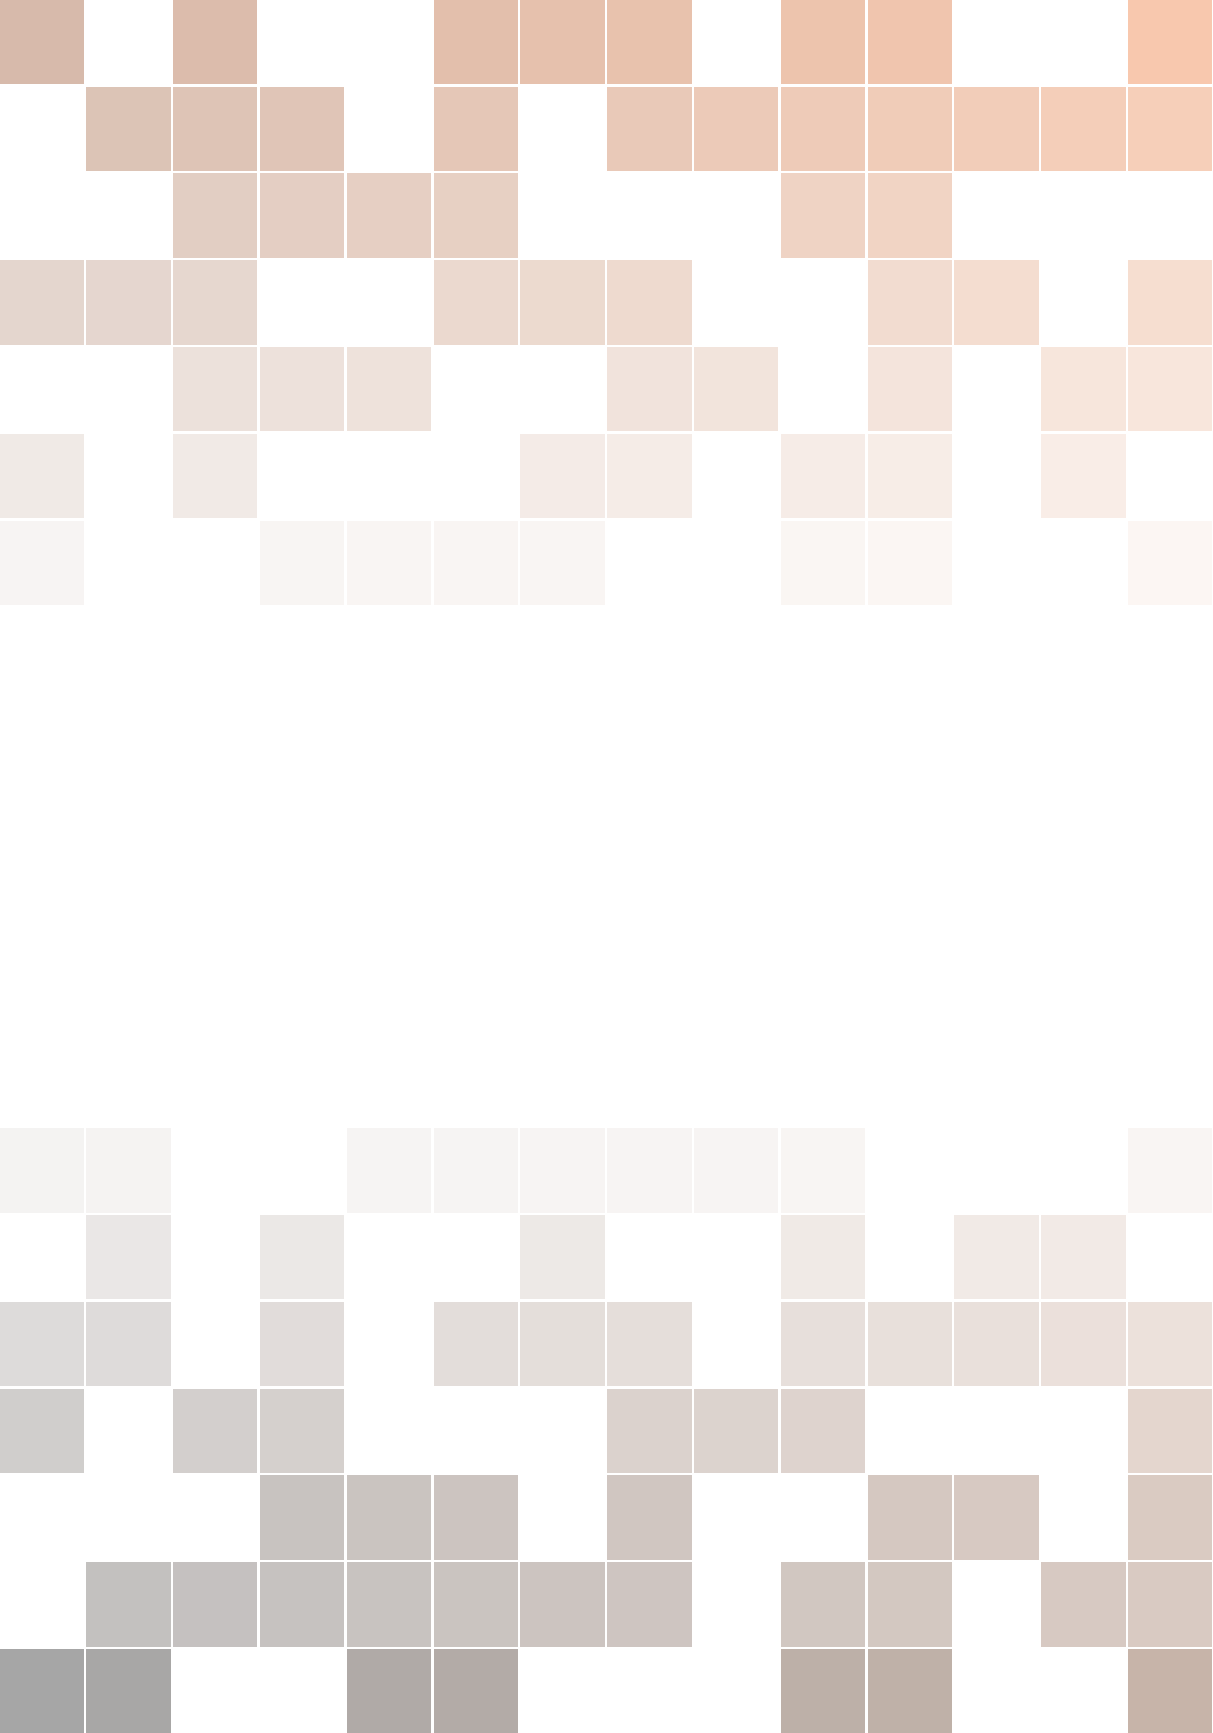
\includegraphics[width=\paperwidth]{background.pdf}};
\draw (current page.center) node [fill=ocre!30!white,fill opacity=0.6,text opacity=1,inner sep=1cm]{\Huge\centering\bfseries\sffamily\parbox[c][][t]{\paperwidth}{\centering Just Enough Robotics\\[15pt] % Book title
%{\Large A Profound Subtitle}\\[20pt] % Subtitle
{\huge Nathan Sprague}}}; % Author name
\end{tikzpicture}
\vfill
\endgroup

%----------------------------------------------------------------------------------------
%	COPYRIGHT PAGE
%----------------------------------------------------------------------------------------

\newpage
~\vfill
\thispagestyle{empty}

Copyright 2023 Nathan Sprague\\ % Copyright notice

This work is licensed under the Creative Commons
Attribution-NonCommercial 4.0 International License. To view a copy of
this license, visit \url{http://creativecommons.org/licenses/by-nc/4.0/} or
send a letter to Creative Commons, PO Box 1866, Mountain View, CA
94042, USA.

This book was generated using the The Legrand Orange Book LaTeX
Template which was developed by Mathias Legrand and is distributed
under the Creative Commons BY-NC-SA 3.0
license. (\url{http://creativecommons.org/licenses/by-nc-sa/3.0/})




%----------------------------------------------------------------------------------------
%	TABLE OF CONTENTS
%----------------------------------------------------------------------------------------

%\usechapterimagefalse % If you don't want to include a chapter image, use this to toggle images off - it can be enabled later with \usechapterimagetrue

\chapterimage{chapter_head_1.pdf} % Table of contents heading image

\pagestyle{empty} % Disable headers and footers for the following pages

\tableofcontents % Print the table of contents itself

\cleardoublepage % Forces the first chapter to start on an odd page so it's on the right side of the book

\pagestyle{fancy} % Enable headers and footers again

%----------------------------------------------------------------------------------------
%	PART
%----------------------------------------------------------------------------------------

%\part{Part One}

%----------------------------------------------------------------------------------------
%	CHAPTER 1
%----------------------------------------------------------------------------------------

\chapterimage{chapter_head_2.pdf} % Chapter heading image

\chapter*{Preface}
\addcontentsline{toc}{chapter}{\textcolor{ocre}{Preface}}

This book is intended to be an accessible introduction to key
algorithmic concepts in autonomous robotics targeted toward
undergraduate computer science students.  It is not intended to be an
exhaustive reference or to provide rigorous mathematical foundations,
derivations or proofs.  The focus is on clear explanations with
extensive examples and visualizations.

This book uses a Python-based pseudocode that is generally very close
to executable Python. I have attempted to steer clear of any idiomatic
Python constructs so that the algorithm listings should be easy to
follow even for those without a background in the Python language.

This book is a work in progress!  It covers several of the central
algorithmic ideas in autonomous robotics, but there are still
significant missing pieces.  In particular, there is currently no
coverage of particle filters, mapping algorithms, or simultaneous
localization and mapping (SLAM). Contributions are welcome!


\chapter*{Acknowledgments}
\addcontentsline{toc}{chapter}{\textcolor{ocre}{Acknowledgments}}

The development of this book was supported by a grant from the Virtual
Library of Virginia (VIVA).

I would also like to thank Dr. Kevin Molloy for providing feedback on
portions of this book and helping me to pilot it in multiple semesters
of CS 354 At James Madison University.


\chapter{Controlling Physical Systems}
\label{chap:pid}

\section{Introduction}

Computer programmers are accustomed to instructions that operate
\emph{instantaneously} and \emph{reliably}. Both assumptions fail when
writing code that controls a physical system. In this chapter we will
take the first steps towards writing programs that can reliably
control physical systems in an unpredictable world.

%% INTRODUCE PID CONTROLLER

\section{Open Loop Control}

\begin{figure}
\begin{center}
\begin{tikzpicture}
[line width=1pt,rotate=0,scale=.4]

\filldraw (2.0, 1) circle (.75);
\filldraw (3.5, 1.0) circle (.75);
\filldraw (5.5, .65) circle (.4);

\draw (1,1) -- (6,1) -- (6,3) -- (1, 3) -- cycle; %body
\draw (1,3) -- (3,3) -- (3,4) -- (1, 4) -- cycle; %cab
\draw (6,1) -- (7,1) -- (6,2.5)  -- cycle; %plow
\draw (-4, .325) -- (10, .325); %rails

\draw[->] (3.5, -2)  node [anchor=north]{$x$} -- (3.5,0);
\draw[->] (7.5, -2)  node [anchor=north]{$g$} -- (7.5,0);

\end{tikzpicture}
\end{center}
\caption{A self-driving locomotive.}
\label{fig:locomotive1}
\end{figure}


Consider the problem of programming a controller for the self-driving
locomotive in Figure \ref{fig:locomotive1}.  In this figure $x$
indicates the starting position of the locomotive and $g$ indicates
the goal location.

Our first attempt at developing a controller might look something like
the following:

\begin{minipage}[c]{0.95\textwidth}
\begin{lstlisting}[label={lst:open-loop},caption={Open Loop Control Algorithm}]
def open_loop(x, g):

    # Calculate the distance to travel.
    d = g - x

    # Cover that distance in one second.
    for one second:
        drive forward at a speed of d/second
\end{lstlisting}
\end{minipage}

Algorithm \ref{lst:open-loop} is an example of an \vocab{open loop
  controller}\index{open loop control}. Open-loop control involves
sending a sequence of control signals that, based on our understanding
of the system we are controlling, should move the system into the
target configuration.

There are problems with Algorithm \ref{lst:open-loop}.  First,
locomotives are \emph{heavy}.  The success of this algorithm relies on
the unrealistic assumption that we can instantaneously changing the
speed from zero to the desired value of $d/s$.  Second, even after the
locomotive reaches the target speed, factors like friction and
mechanical imperfections will make it impossible to perfectly maintain
that speed. Over time, small errors in speed will result in
significant errors in the final position.


\section{Closed Loop Control}

\begin{figure}
\begin{center}
\begin{tikzpicture}
[line width=1pt,rotate=0,scale=.4]

\filldraw (2.0, 1) circle (.75);
\filldraw (3.5, 1.0) circle (.75);
\filldraw (5.5, .65) circle (.4);

\draw (1,1) -- (6,1) -- (6,3) -- (1, 3) -- cycle; %body
\draw (1,3) -- (3,3) -- (3,4) -- (1, 4) -- cycle; %cab
\draw (6,1) -- (7,1) -- (6,2.5)  -- cycle; %plow
\draw (-4, .325) -- (10, .325); %rails

\draw[->] (3.5, -1.5)  node [anchor=north]{$x(t)$} -- (3.5,0);
\draw[->] (7.5, -1.5)  node [anchor=north]{$g(t)$} -- (7.5,0);

\draw[|-|] (3.5, -3.3)[dashed] -- (7.5,-3.3) node[pos=0.5,below]{$e(t)$};



\end{tikzpicture}
\end{center}
\caption{A self-driving locomotive.}
\label{fig:locomotive2}
\end{figure}


The problems with the naive controller in Algorithm
\ref{lst:open-loop} can be avoided by using \vocab{closed loop
  control}\index{closed loop control}.  Closed loop controllers
continuously monitor the current error in the system and update the
control signal to push the error toward zero.  This approach tends to
be more reliable because the controller responds to the actual state
of the system and is able to make adjustments when the system fails to
behave as expected.


The PID (\textbf{P}roportional, \textbf{I}nverse, \textbf{D}erivative)
controller is the classic example of closed loop control.  The next
several sections will introduce the PID controller by describing each
of these three terms.  The following table outlines the notation
that will be used (Figure
\ref{fig:locomotive2} also uses this notation).


\begin{tabular}{l p{4in}}
$x(t)$ &

  The state of the system at time $t$.  In the case of the locomotive
  this is the position on the track. More generally, this could
  describe any state variable that we are interested in controlling.
  This could be the temperature of a room or the altitude of a
  rocket.

  For now, we will assume that state information is provided by a
  reliable sensor.  In future chapters we will consider the problem of
  estimating this value when sensors are absent or unreliable.\\

$g(t)$ & Goal state at time $t$. \\

$e(t)$ & Error at time $t$.

 We will let $e(t) = g(t) - x(t)$. In the case of the locomotive, this
 value is zero when the locomotive is at the goal position, positive
 when the locomotive is to the left of the goal, and negative if the
 locomotive overshoots and ends up to the right of the goal. \\

$u(t)$ & The control signal at time $t$. The interpretation of $u(t)$
 depends on system we are attempting to control.  In some cases $u(t)$
 might represent a low-level control signal like the voltage sent to a
 motor. In other cases we may be working with a robot that allows us
 to directly specify a desired velocity or acceleration.

 In the case of our hypothetical locomotive, we will assume we have an
 API provides a \verb+throttle+ function that takes a number in the
 range (-100, 100) where +100 represents ``full speed ahead'' and -100
 represents ``full reverse''.
\end{tabular}

\subsection{Proportional Control}

Mathematically, we can think of the problem of developing a controller
as finding an expression for $u(t)$ in terms of $e(t)$.  One simple
possibility is to follow the intuition that the magnitude of the control
signal should be proportional to the current error.  In the locomotive
example, this means we should apply more throttle when the locomotive
is far from the goal location, and ease off as the locomotive gets
closer.  This idea can be expressed as follows:

\begin{equation}
 u(t) = K_p e(t)
\end{equation}

The value $K_p$ is referred to as a \vocab{gain}\index{gain} term. This is a
constant that determines how large the control signal will be for a
particular error value.  Doubling the gain doubles the magnitude of
the control signal.  Developing a successful controller involves
selecting an appropriate gain value, either by analyzing the system or
through trial and error.

Algorithm \ref{lst:proportional} shows how we can implement a
proportional controller for the locomotive example.


\begin{minipage}[c]{0.95\textwidth}
\begin{lstlisting}[label={lst:proportional},caption={Proportional Control Algorithm}]
def p_controller(train, g, K_P):
    while True:
        e = g - train.x
        u = K_P * e
        train.throttle(u)

\end{lstlisting}
\end{minipage}



Figure \ref{fig:p_result} shows the result of using a proportional
controller to implement our locomotive controller using two different
values of $K_P$.

\begin{figure}
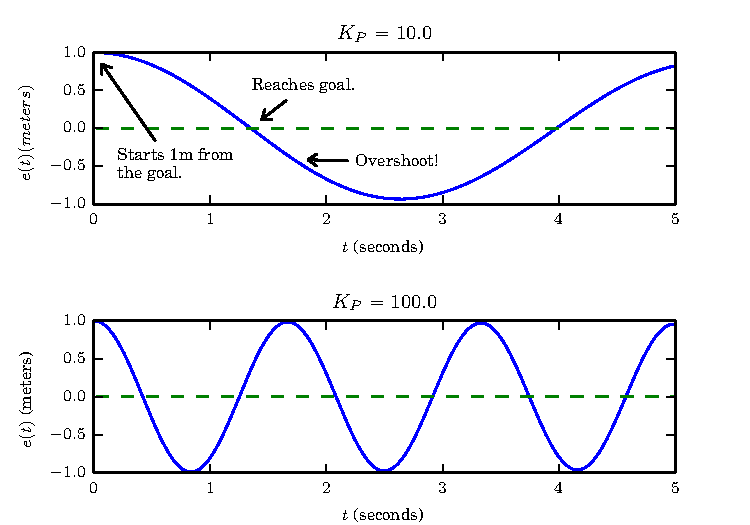
\includegraphics{pid/figs/p_result.pdf}
\caption{Locomotive position error over time for two different values of $K_P$.} 
\label{fig:p_result}
\end{figure}

These results are not very satisfying. The locomotive overshoots the
goal and then over-corrects, driving back and forth indefinitely.
Changing the value of $K_P$ doesn't solve the problem, it only changes
the period of the oscillations.


\subsection{Adding a Derivative Term}

One problem with our proportional controller is that it only considers
the position of the locomotive, not the speed.  Intuitively, it seems
that if the error is already decreasing quickly, we should reduce the
control signal to avoid overshooting the goal.  Conversely, if the
error is still increasing in spite of the proportional control, we should
further increase the magnitude of the control signal.  These
intuitions can be captured by adding a derivative term to the
controller:

\begin{equation}
u(t) = K_p e(t) +
\tikz[baseline]{
    \node[draw=red,rounded corners,anchor=base] (m1)
    {$\displaystyle K_d \diff{e(t)}{t}$};
    \node[above of=m1] (l1) {derivative term};
    \draw[-,red] (l1) -- (m1);
}
\label{eq:pd_equation}
\end{equation}


The term $\diff{e(t)}{t}$ describes the rate of change in the error.
This is negative if the error is decreasing and positive if the error
is increasing.  The value $K_d$ is a gain that is used to tune
the impact of the derivative term.

Using the derivative term requires us to know $\diff{e(t)}{t}$, but
sensors don't usually provide direct access to this value.  Instead,
we need to estimate it by tracking the change in error over time.
Even though the physical systems we are controlling operate
continuously, our algorithms necessarily perform their steps at
discrete time intervals.  Assuming our controller is updated every
$\Delta t$ seconds, we can estimate the derivative as the slope
between the two most recent error values:

\begin{equation}
\diff{e(t)}{t} \approx \frac{e(t) - e(t - \Delta t)}{\Delta t}
\label{eq:diff_approx}
\end{equation}


% Issue: approximation can cause problems if delta t is short and 
% measurements are noisy.

%% \begin{tikzpicture} 
%% \begin{axis}[ 
%% height=5cm, 
%% width=5cm, 
%% xlabel=$t$, 
%% ylabel=$e(t)$,
%% xmin=0, 
%% xmax=2, 
%% samples=10,
%% smooth,] 

%% \addplot [domain=0:2,mark=]{10 *x^3 + 1 - 3* x^2}; 

%% \end{axis} 
%% \end{tikzpicture}


Discrete approximations like this are common in robotics and in
other areas of scientific computing but they aren't always made
explicit.  It takes some experience to get comfortable moving from
continuous to discrete formulations. Algorithm
\ref{lst:proportional_deriv} illustrates how we can use the discrete
approximation in Equation \ref{eq:diff_approx} to implement the
control algorithm described in Equation \ref{eq:pd_equation}. 


\begin{minipage}[c]{0.95\textwidth}
\begin{lstlisting}[label={lst:proportional_deriv},caption={Proportional Derivative Control Algorithm}]
def pd_controller(train, g, K_P, K_D):
    e_prev = g - train.x
    while True:
        e = g - train.x
        dedt = (e - e_prev) / train.dt  # Equation 1.3
        u = K_P * e + K_D * dedt
        train.throttle(u)
        e_prev = e
\end{lstlisting}
\end{minipage}


\begin{figure}
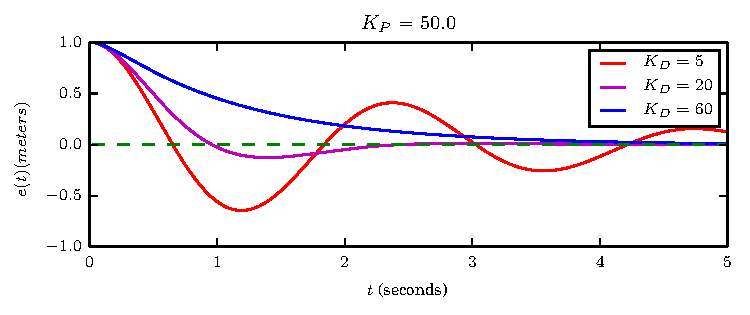
\includegraphics{pid/figs/pd_result.pdf}
\caption{Locomotive position error over time for three different
  values of $K_D$.}
\label{fig:pd_result}
\end{figure}

Figure \ref{fig:pd_result} shows the result of introducing the derivative term in our
controller.  For appropriate values of $K_D$ the oscillations are
damped, and the locomotive settles at the goal location.

\subsection*{Stop and Think}

\begin{exercise}
  The \verb+while+ loop in Listing \ref{lst:proportional_deriv} does
  not include any explicit delays.  It is written under the assumption
  that methods called on the \verb+train+ object will only return
  after an appropriate delay.  What could go wrong if this is not the
  case?  In other words, what will happen if the execution time of the
  loop is much shorter than \verb+train.dt+?
\end{exercise}



\subsubsection{Droop}


\begin{figure}
\begin{center}
\begin{tikzpicture}
[line width=1pt,rotate=8,scale=.4]

\filldraw (2.0, 1) circle (.75);
\filldraw (3.5, 1.0) circle (.75);
\filldraw (5.5, .65) circle (.4);

\draw (1,1) -- (6,1) -- (6,3) -- (1, 3) -- cycle; %body
\draw (1,3) -- (3,3) -- (3,4) -- (1, 4) -- cycle; %cab
\draw (6,1) -- (7,1) -- (6,2.5)  -- cycle; %plow
\draw (-4, .325) -- (10, .325); %rails

\draw[->] (3.5, -2)  node [anchor=north]{$x(t)$} -- (3.5,0);
\draw[->] (7.5, -2)  node [anchor=north]{$g(t)$} -- (7.5,0);

\draw[|-|] (3.5, -3.5)[dashed] -- (7.5,-3.5) node[pos=0.5,below]{$e(t)$};
\end{tikzpicture}
\end{center}
\caption{Locomotive on a hill.}
\label{fig:train_hill}
\end{figure}

What happens when we try to apply the same controller when the
locomotive is located on a slight incline as shown in Figure
\ref{fig:train_hill}?  In this situation, which is illustrated in
Figure \ref{fig:pd_droop}, the locomotive never quite
reaches the goal position.  The locomotive comes to rest at the point
where the proportional force applied by the controller is exactly
counterbalanced by gravity.  Increasing $K_p$ will move the stationary
point closer to the goal, but this controller will never drive the
error all the way to zero.  The situation where the proportional term
is not sufficient to drive the error term to zero is sometimes
referred to as ``droop''. 

\begin{figure}
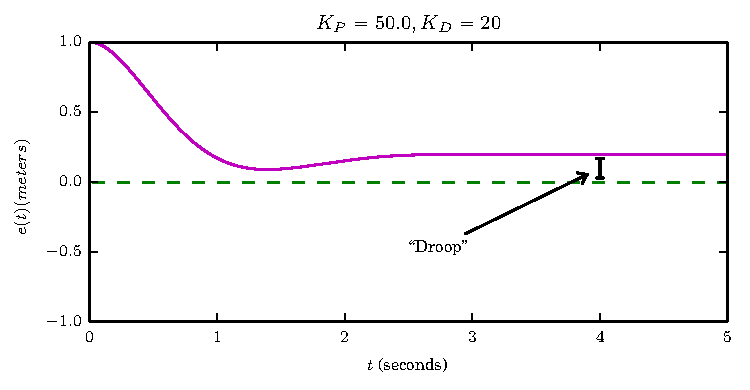
\includegraphics{pid/figs/pd_result_hill.pdf}
\caption{Locomotive position error over time for the PD locomotive
  controller when the locomotive is on an incline.  The locomotive
  stops short of the goal at the point where the control output is
  counter-balanced by gravity.}
\label{fig:pd_droop}
\end{figure}



\subsection{Adding an Integral Term}

The problem of droop can be addressed by adding one more term to our
controller:

\begin{equation}
u(t) = K_P e(t) +
\tikz[baseline]{
    \node[draw=red,rounded corners,anchor=base] (m1)
    {$\displaystyle K_I  \int_0^t e(\tau)d\tau $};
    \node[above of=m1] (l1) {integral term};
    \draw[-,red] (l1) -- (m1);
}
+ K_D \diff{e(t)}{t} 
\end{equation}

\noindent Where the derivative term allows the controller to look forward in
time, the integral term allows the controller to look backwards in
time.  The integral $\int_0^t e(\tau)d\tau$ essentially ``stores up''
the error that the system sees over time.  As long as the error fails
to reach zero, $\int_0^t e(\tau)d\tau$ will steadily increase in
magnitude.

As with the derivative, the integral value is not available directly,
but must be estimated from discrete samples.  In this case, the
integral can be estimated using a summation that adds the current
error value at each time step:


\begin{equation}
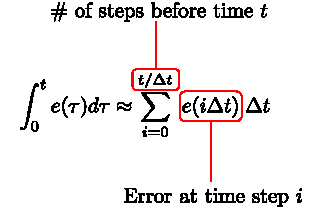
\includegraphics{pid/figs/annotated_summation.pdf}
%\int_0^t e(\tau)d\tau \approx \sum_{i=0}^{t/\Delta t} e(i \Delta t) \Delta t 
\end{equation}

%% \begin{tikzpicture}
%% \begin{axis}[
%%  ylabel near ticks,
%%     xtick={0,1,3,5,7,9,11,13,15,17},ytick={0,...,1.5},
%%     xmax=18,ymax=1.2,ymin=0,xmin=0,
%%     enlargelimits=true,
%%     axis lines=middle,
%%     clip=false,
%%     domain=0:17,
%%     xlabel near ticks,
%%     xlabel={$t$},
%%     ylabel={$e(t)$},
%%     ]

%% \addplot [draw=red, fill=red!10, ybar interval, samples=9, domain=1:17]
%%     {x^-1}\closedcycle;

%% \addplot[smooth, thick,domain=1:17,samples=40]{x^-1};

%% \end{axis}
%% \end{tikzpicture}




\begin{minipage}[c]{0.95\textwidth}
\begin{lstlisting}[label={lst:pid},caption={PID Control Algorithm}]
def pid_controller(train, g, K_P, K_I, K_D):

    e_prev = g - train.x
    e_sum = 0             # accumulator for integral term
    while True:
        e = g - train.x
        e_sum = e_sum + e * train.dt   # From Equation 1.5
        dedt = (e - e_prev) / train.dt # Equation 1.3 
        u = K_P * e   +   K_I * e_sum   +   K_D * dedt
        train.throttle(u)
        e_prev = e

\end{lstlisting}
\end{minipage}


\begin{figure}
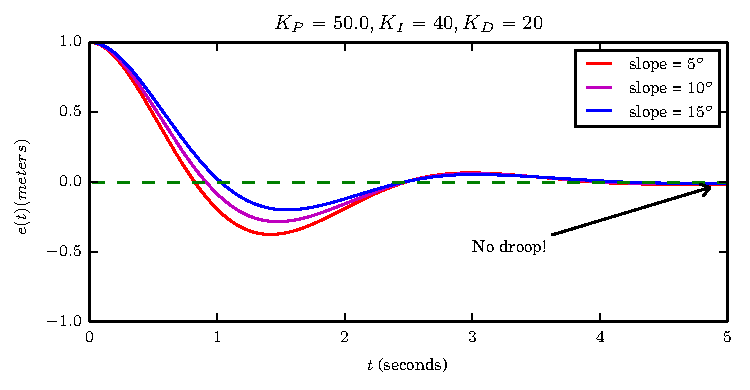
\includegraphics{pid/figs/pid_result_hill.pdf}
\caption{Locomotive position error over time for a different slopes.
  With appropriate gain values the PID controller reliably moves the
  locomotive to the goal location.}
\label{fig:pid_result}
\end{figure}


Algorithm \ref{lst:pid} illustrates a complete PID controller.  Figure
\ref{fig:pid_result} shows the result of adding an integral term to
our locomotive controller.  With an appropriate value of $K_I$, the
resulting controller reliably moves the locomotive to the goal regardless
of the slope.

\subsection*{Stop and Think}
\begin{exercise}
  Practical implementations of PID controllers often place a cap on
  the amount of error that can be accumulated in the integral term of
  the controller.  Why do you think this is necessary?  What could go
  wrong if the controller were to start out far from the goal
  configuration, accumulating a large amount of error before the goal
  is reached?
\end{exercise}

\begin{exercise}
  The process outlined above for tuning the PID gain terms is ad-hoc:
  we just experimented with different values until the behavior looked
  right. A more rigorous approach would require a quantitative way to
  evaluate the success of a particular PID controller.  Can you think
  of some quantitative measurements that might be useful for comparing
  two controllers? 
\end{exercise}


\begin{exercise}
  Consider the following graph of error as a function of
  time. Assuming that this system is being controlled by a PID
  controller, how would you suggest what the gain terms be modified?
  \begin{center}
  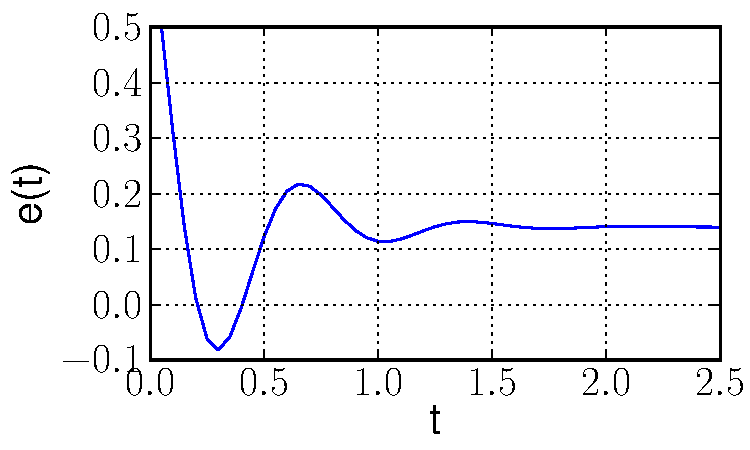
\includegraphics[width=2.2in]{pid/figs/pid_stop_and_think1.pdf}
  \end{center}
\end{exercise}

\begin{exercise}
  Consider the following graph of error as a function of
  time. Assuming that this system is being controlled by a PID
  controller, how would you suggest what the gain terms be modified?
  \begin{center}
  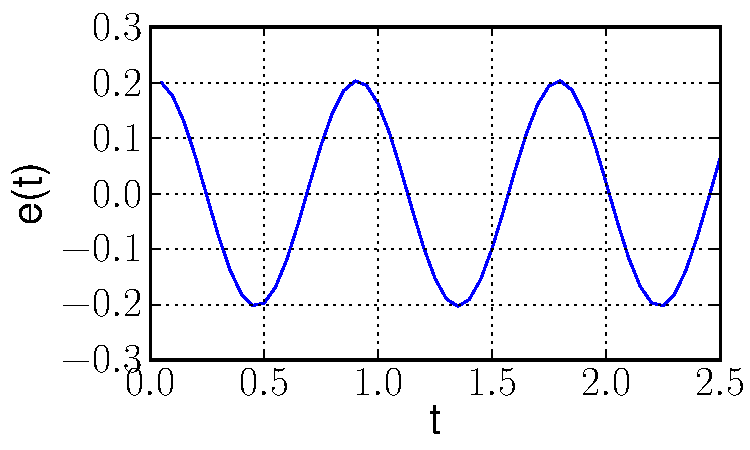
\includegraphics[width=2.2in]{pid/figs/pid_stop_and_think2.pdf}
  \end{center}
\end{exercise}


%% \subsection{complictions}
%% Calculating derivative
%% Storing derivatives
%% Tuning gains

%% restricting the magnitude

\section{Proportional Robot Control}
\label{sec:p_robot_control}
%---------------------------------
% MACROS FOR DRAWING ROBOTS
%--------------------------------
\newcommand{\drawwheel}[2]{
\begin{scope}[shift={(#1,#2)}]
\filldraw (.3,.1) -- (.3,-.1) -- (-.3,-.1) -- (-.3,.1) -- cycle; 
\end{scope}
}

%Draw robot at x, y, theta
\newcommand{\drawdiffrobot}[4]{
\begin{scope}[shift={(#1,#2)},rotate=#3,scale=#4]
\draw (0,0) circle (1);
\draw[thick,->] (0,0) -- (.7,0);
\drawwheel{0}{.7}
\drawwheel{0}{-.7}
\end{scope}
}

%---------------------------------
%--------------------------------



You may feel that a self-driving locomotive is a disappointingly
simple robot: all it can do is move backward and forward along a
linear track.  Don't fear, this book will mostly focus on mobile
robots that are able to move freely in multiple dimensions.  In this
section we will develop a proportional controller for driving a wheeled
robot to a goal location as illustrated in Figure
\ref{fig:diff_robot}.



\begin{figure}[h]
\begin{center}
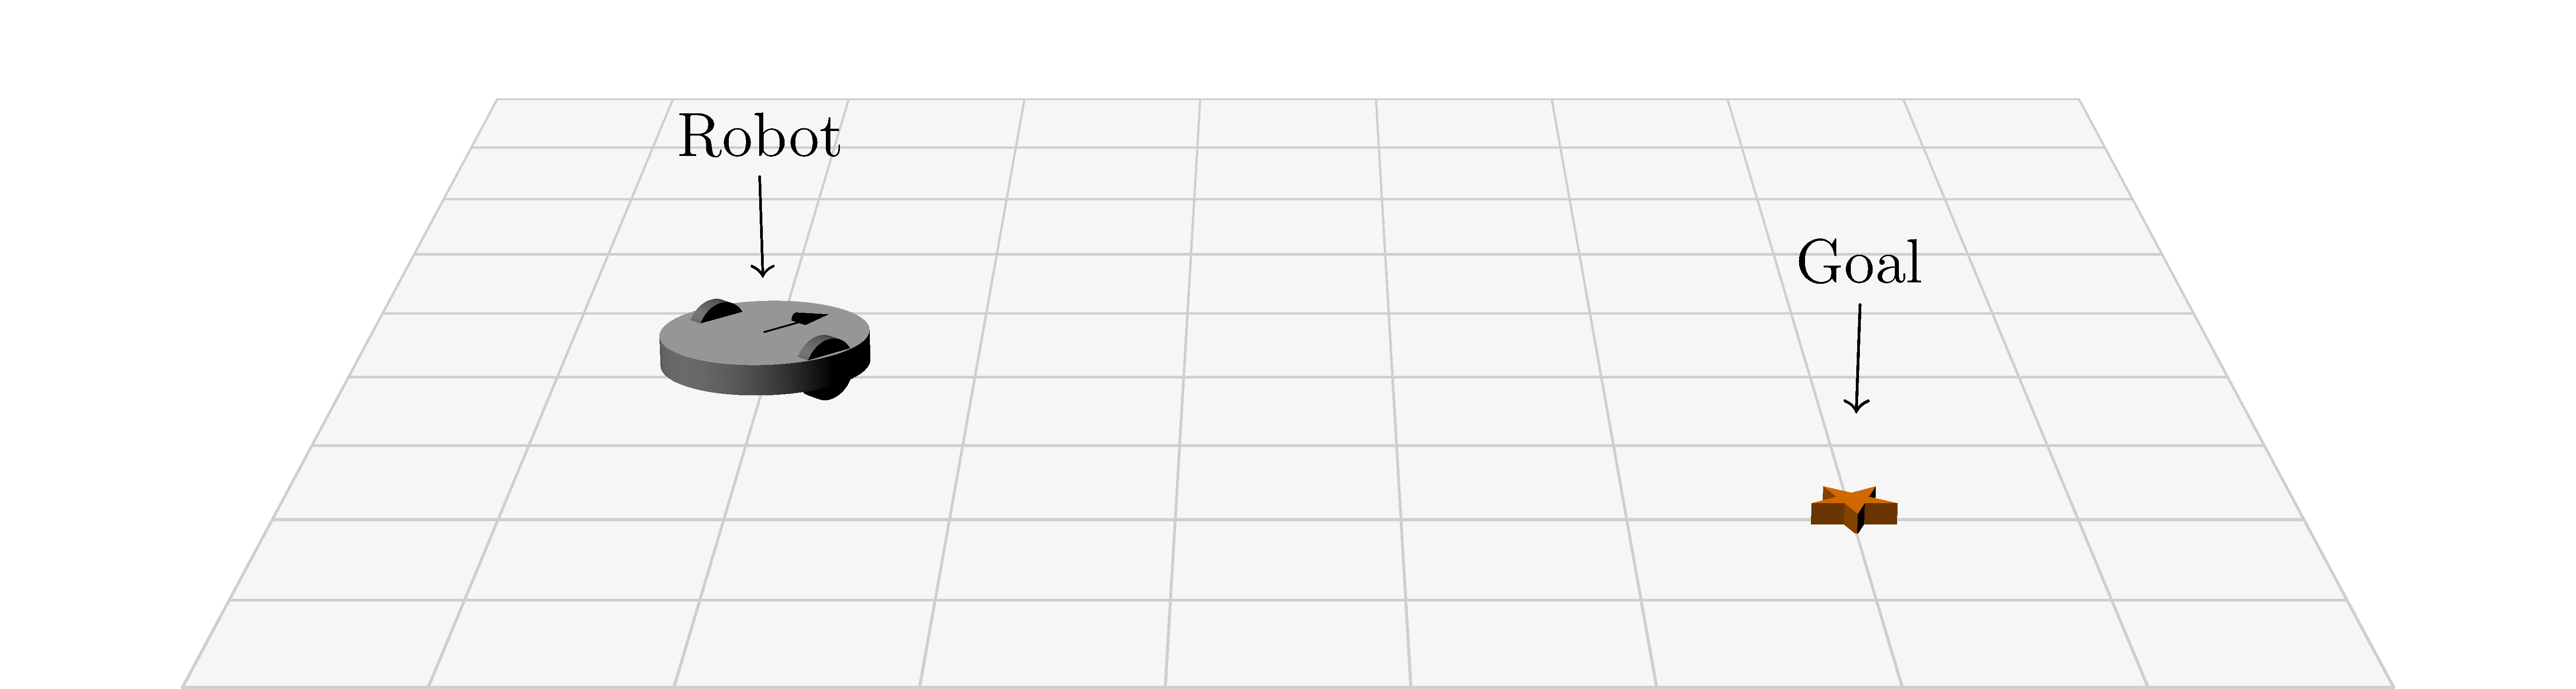
\includegraphics{pid/figs/3drobot.png}
\end{center}
\caption{Differential drive robot.}
\label{fig:diff_robot}
\end{figure}



%% \begin{figure}[h]
%% \begin{center}
%% \begin{tikzpicture}

%% \coordinate[] (G) at (3.5,1);
%% \coordinate[] (R) at (1, 2);

%% %Axes
%% \draw[thick,->] (0,0) -- (4.5,0) node[anchor=north ] {$x$};
%% \draw[thick,->] (0,0) -- (0,4.5) node[anchor= east] {$y$};

%% %Robot
%% \drawdiffrobot{1}{2}{45}{.4}

%% %Robot label
%% \draw[->,shorten >=0.6cm] (1.78,3.08) node[above] {Robot} -- (R);

%% %Star
%% \draw (G) node[draw,star,star points=5,star point ratio=.5]{};

%% %Star label
%% \draw[->,shorten >=0.4cm] (4.5, 2) node[above] {Goal} -- (G);

%% \end{tikzpicture}
%% \end{center}
%% \caption{Overhead view of a differential drive robot.  The small black
%%   rectangles represent the wheels.}
%% \label{fig:diff_robot}
%% \end{figure}


This is an example of a \vocab{differential drive}\index{differential
  drive} robot.  This type of robot has two independently controllable
wheels.  When both wheels are rotated in the same direction at the
same speed the robot moves directly forward or backward.  If both
wheels are turned in opposite directions the robot will rotate in
place.  The robot can follow a curved path by rotating each wheel at a
different speed.

Since it is not intuitive to steer a differential drive robot by
directly controlling the wheel velocities, the driver software for
such robots often accepts commands specifying two velocity values: $v$
and $w$, where $v$ is the forward velocity in meters/second and $w$ is
the rotational velocity in radians/second. 
%TODO call forward to kinematics chapter where this translation will
%be described.

\begin{figure}[h!]
\begin{center}
\begin{tikzpicture}

\node[] (G) at (3.5,1){};
\coordinate[] (R) at (1, 2);
\coordinate[] (xaxis) at (4.5,0);
\coordinate[] (yaxis) at (0, 4.5);

% Axes
\draw [<->,thick] (yaxis)node[label=left:$y$] {} |- 
(xaxis)node[label=below:$x$] {};

% Robot
\drawdiffrobot{1}{2}{45}{.4}

\begin{scope}[draw=blue,text=blue]
% x, y coordinates
\draw[dashed,shorten >=0.4cm] (yaxis |- R) node[left] {$y_r$} -- (R);
\draw[dashed,shorten >=0.4cm] (xaxis -| R) node[below] {$x_r$} -- (R);

% angle:
\coordinate[] (A) at ($(R) + (1.75,1.75)$);
\coordinate[] (C) at ($(R) + (2,0)$);
\draw[dashed,->,shorten <=0.4cm] (R) node[above] {} -- (A);
\draw[dashed,->,shorten <=0.4cm] (R) node[above] {} -- (C);
\tkzMarkAngle[arc=l,size=1.0,arrows=->](C,R,A)
\tkzLabelAngle[pos = 1.3](C,R,A){$\Theta_r$}
\end{scope}

%Star
\draw (G) node[draw,star,star points=5,star point ratio=.5]{};

\begin{scope}[draw=green,text=green]
% x, y coordinates
\draw[dashed] (yaxis |- G) node[left] {$y_g$} -- (G);
\draw[dashed] (xaxis -| G) node[below] {$x_g$} -- (G);
\end{scope}


\end{tikzpicture}
\end{center}
\caption{Overhead view of the robot and goal.}
\label{fig:diff_coords}
\end{figure}

Figure \ref{fig:diff_coords} illustrates the parameterization of the
control problem.  The pose of the robot is specified with three
numbers: $(x_r, y_r, \Theta_r)$, where the $x_r$ and $y_r$ coordinates
specify the position of the center of the robot with respect to some
fixed point in the room and the $\Theta_r$ value indicates the robot's
heading.  Heading values (in radians) are in the interval $[-\pi,
  \pi]$, where $\Theta_r = 0$ indicates that the robot is pointing
along (or parallel to) the $x$-axis.
As the robot turns counterclockwise, $\Theta_r$ increases.
The value of $\Theta_r$ in figure
Figure \ref{fig:diff_coords} is approximately $\frac{\pi}{4}$ (or
$45^o$).



We can solve this control problem by creating two separate
proportional controllers that will operate simultaneously: one
controller to output a rotational velocity that turns the robot toward
the goal, the other to output a forward velocity that keeps the robot
moving forward until it reaches the goal.


\begin{figure}[h!]
\begin{center}
\begin{tikzpicture}

\node[] (G) at (3.5,1){};
\coordinate[] (R) at (1, 2);
\coordinate[] (xaxis) at (4.5,0);
\coordinate[] (yaxis) at (0, 4.5);

% Axes
\draw [<->,thick] (yaxis)node[label=left:$y$] {} |- 
(xaxis)node[label=below:$x$] {};

% Robot
\drawdiffrobot{1}{2}{45}{.4}

% Star
\draw (G) node[draw,star,star points=5,star point ratio=.5]{};

% Triangle
\coordinate[] (A) at (R -| G);
\draw (A) -- node[above] {$x_g - x_r$} (R) -- (G) -- 
node[right] {$y_g - y_r$}(A);

% Label angle.
\tkzMarkAngle[arc=l,size=1.0,arrows=<-](G,R,A)
\tkzLabelAngle[pos = 1.3](G,R,A){$\Theta_g$}
\end{tikzpicture}

\end{center}
\caption{Goal angle calculations}
\label{fig:goal_angle}
\end{figure}

The first step in developing the rotational controller is determining
the desired angle for the robot.  The problem is illustrated in Figure
\ref{fig:goal_angle}. Determining $\Theta_g$ from the positions of the
robot and goal requires some trigonometry:

\begin{equation}
\Theta_g = \tan^{-1}  \frac{y_g - y_r}{x_g - x_r}
\label{eq:calc_theta_g}
\end{equation} 

Actually, this won't \emph{quite} give us what we want.  Equation
\ref{eq:calc_theta_g} doesn't distinguish between the case when both
the numerator and denominator are positive and the case when they are
both negative.  This means that a goal above and to the right of the
robot will result in the same angle as an object below and to the
left.  The math libraries for many programming languages address this
difficulty by providing a function named \texttt{atan2} that takes the
numerator and denominator as separate arguments and correctly
calculates the angle taking the signs of the arguments into account.
A Python implementation might look something like the following:

\begin{center}
\begin{verbatim}
theta_g = math.atan2(y_g - y_r, x_g - x_r)
\end{verbatim}
\end{center}

Given that we can calculate a target angle, our rotational controller
can be specified using the formula for a proportional controller
(dropping the time index for clarity):


\begin{equation}
 w = K_{P_w} (\Theta_g - \Theta_r)
\end{equation}

Unfortunately, subtracting angles in a sensible way requires some
caution.  Consider the situation in Figure \ref{fig:angle_problem}.
Naively calculating the error by subtracting the two angles gives us
$.9 \pi - (-.9\pi) = 1.8\pi$.  Plugging this into our proportional
controller will result in a hard left turn.  This isn't exactly wrong:
it \emph{is} possible for the robot to point toward the goal by
turning to the left.  However, it clearly makes more sense to select
the smaller angle between our current heading and the target heading and
have the robot turn right.
We will use the symbol $\ominus$ to indicate an angle subtraction
operation that has this effect.  With this modification we can
completely specify the control scheme for the differential drive
robot.

\begin{align} 
 w =& K_{P_w} (\Theta_g \ominus \Theta_r) \label{eq:diff_rot}\\
 v =& K_{P_v} \sqrt{(y_g - y_r)^2 + (x_g - x_r)^2} \label{eq:diff_vel}
\end{align}

Equation \ref{eq:diff_vel} expresses the idea that the robot's forward
velocity should be proportional to its Euclidean distance from the
goal.  Since this velocity control is independent of the angle, the
robot may initially move away from the goal.  We could address through
a more complicated control mechanism, but the point here is to
illustrate a simple example of proportional control.  Figure
\ref{fig:diff_demo} shows several example trajectories of a simulated
differential drive robot under the control scheme presented in
Equations \ref{eq:diff_rot} and \ref{eq:diff_vel}.


\begin{figure}[h!]
\begin{center}
\begin{tikzpicture}

\node[] (G) at (1,2.81){};
\coordinate[] (R) at (3.5, 2);
\coordinate[] (xaxis) at (4.5,0);
\coordinate[] (yaxis) at (0, 4.5);

% Axes
\draw [<->,thick] (yaxis)node[label=left:$y$] {} |- 
(xaxis)node[label=below:$x$] {};

% Robot
\drawdiffrobot{3.5}{2}{-162}{.4}

% Star
\draw (G) node[draw,star,star points=5,star point ratio=.5]{};

% angle:
\coordinate[] (C) at ($(R) + (2,0)$);
\draw[dashed,->,shorten <=0.4cm] (R) node[above] {} -- (C);

% goal angle
\begin{scope}[draw=green,text=green]
\draw[dashed,->,shorten <=0.4cm] (R) node[above] {} -- (G);
\tkzMarkAngle[arc=l,size=1.0,arrows=->](C,R,G)
\tkzLabelAngle[pos = 1.3](G,R,C){$\Theta_g = .9\pi$}
\end{scope}

% robot angle
\coordinate[] (D) at ($(R) + (-2,-.65)$);
\begin{scope}[draw=blue,text=blue]
\draw[dashed,->,shorten <=0.4cm] (R) node[above] {} -- (D);
\tkzMarkAngle[arc=l,size=.8,arrows=<-](D,R,C)
\tkzLabelAngle[pos = 1.3](D,R,C){$\Theta_r = -.9\pi$}
\end{scope}

\end{tikzpicture}

\end{center}
\caption{The robot can either turn $.2\pi$ radians clockwise, or $1.8\pi$ radians
  counterclockwise to face the goal. We want a difference operation
  that always returns the smaller angle. }
\label{fig:angle_problem}
\end{figure}


\begin{figure}[h!]
\begin{center}
\begin{tikzpicture}
\begin{axis}[unit vector ratio*=1 1 1,
axis x line=bottom,
axis y line=left,
xmin=1.5,xmax=9,
ymin=1.5,ymax=9.25,
ticks=none]
\addplot[color=red,smooth] coordinates {
(7.43698072433, 3.02302646637)
(7.30944538116, 2.8852930069 )
(7.12435770035, 2.84149670601)
(6.90518760681, 2.88129091263)
(6.73256778717, 2.96469521523)
(6.57478523254, 3.07387018204)
(6.42918539047, 3.19893813133)
(6.27081918716, 3.35729455948)
(6.14221286774, 3.49984359741)
(6.01804590225, 3.6462829113)
(5.87715482712, 3.82042050362)
(5.75883102417, 3.97162556648)
(5.64206647873, 4.12403869629)
(5.52646827698, 4.27733898163)
(5.39273405075, 4.45703601837)
(5.27888917923, 4.61164283752)
(5.17062282562, 4.75992250443)
(5.10430622101, 4.85154008865)
(5.05697059631, 4.9176197052)
(5.03474617004, 4.949010849)
(5.02116727829, 4.96842718124)
 };


\addplot[color=red,smooth] coordinates {
(8.22, 5.54)
(8.13, 5.71)
(7.98, 5.81)
(7.79, 5.87)
(7.57, 5.88)
(7.38, 5.86)
(7.19, 5.82)
(7.01, 5.77)
(6.79, 5.70)
(6.61, 5.64)
(6.43, 5.58)
(6.25, 5.51)
(6.04, 5.43)
(5.86, 5.36)
(5.68, 5.28)
(5.48, 5.20)
(5.30, 5.13)
(5.18, 5.08)
(5.11, 5.05)
(5.06, 5.03)
(5.04, 5.02)
};

\addplot[color=red,smooth] coordinates {
(6.50, 8.72)
(6.70, 8.77)
(6.84, 8.65)
(6.91, 8.47)
(6.92, 8.28)
(6.88, 8.06)
(6.81, 7.88)
(6.73, 7.71)
(6.64, 7.54)
(6.53, 7.34)
(6.44, 7.18)
(6.33, 7.01)
(6.21, 6.82)
(6.11, 6.66)
(6.00, 6.50)
(5.90, 6.34)
(5.77, 6.16)
(5.67, 6.00)
(5.56, 5.84)
(5.45, 5.68)
(5.33, 5.49)
(5.22, 5.33)
(5.14, 5.20)
(5.08, 5.13)
(5.04, 5.06)
(5.03, 5.04)
};
\addplot[color=red,smooth] coordinates {
(3.34, 7.82)
(3.53, 7.80)
(3.70, 7.71)
(3.87, 7.56)
(3.98, 7.41)
(4.09, 7.25)
(4.18, 7.08)
(4.28, 6.88)
(4.35, 6.70)
(4.43, 6.53)
(4.51, 6.32)
(4.58, 6.14)
(4.65, 5.96)
(4.72, 5.78)
(4.79, 5.57)
(4.86, 5.39)
(4.91, 5.24)
(4.95, 5.15)
(4.97, 5.08)
(4.98, 5.05)
(4.99, 5.03)
};
\addplot[color=red,smooth] coordinates {
(2.49, 5.93)
(2.51, 5.74)
(2.61, 5.58)
(2.78, 5.43)
(2.95, 5.34)
(3.13, 5.27)
(3.31, 5.22)
(3.53, 5.17)
(3.72, 5.13)
(3.91, 5.10)
(4.10, 5.08)
(4.32, 5.05)
(4.51, 5.03)
(4.70, 5.02)
(4.83, 5.01)
(4.90, 5.00)
(4.94, 5.00)
(4.96, 5.00)
};
\addplot[color=red,smooth] coordinates {
(2.50, 3.17)
(2.69, 3.14)
(2.88, 3.16)
(3.09, 3.24)
(3.25, 3.33)
(3.41, 3.44)
(3.56, 3.56)
(3.73, 3.71)
(3.87, 3.84)
(4.01, 3.97)
(4.17, 4.13)
(4.30, 4.27)
(4.44, 4.41)
(4.57, 4.54)
(4.73, 4.71)
(4.83, 4.82)
(4.90, 4.89)
(4.94, 4.93)
(4.97, 4.96)
(4.98, 4.98)
};

\addplot[color=red,smooth] coordinates {
(5.21, 2.26)
(5.08, 2.13)
(4.89, 2.15)
(4.72, 2.29)
(4.64, 2.46)
(4.59, 2.64)
(4.57, 2.84)
(4.58, 3.06)
(4.60, 3.25)
(4.63, 3.44)
(4.66, 3.63)
(4.71, 3.85)
(4.75, 4.04)
(4.79, 4.22)
(4.85, 4.44)
(4.89, 4.63)
(4.93, 4.77)
(4.96, 4.86)
(4.98, 4.92)
(4.98, 4.95)
(4.99, 4.97)
};

\node[inner sep=0pt] (russell) at (axis cs:7.437,3.023)
    {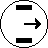
\includegraphics[angle=251,scale=.6]{pid/robot.pdf}};

\node[inner sep=0pt] (russell) at (axis cs:8.22,5.54)
    {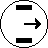
\includegraphics[angle=96,scale=.6]{pid/robot.pdf}};

\node[inner sep=0pt] (russell) at (axis cs:6.50,8.72)
    {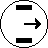
\includegraphics[angle=57,scale=.6]{pid/robot.pdf}};

\node[inner sep=0pt] (russell) at (axis cs:3.34,7.82)
    {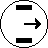
\includegraphics[angle=9,scale=.6]{pid/robot.pdf}};

\node[inner sep=0pt] (russell) at (axis cs:2.49,5.93)
    {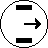
\includegraphics[angle=258,scale=.6]{pid/robot.pdf}};

\node[inner sep=0pt] (russell) at (axis cs:2.50,3.17)
    {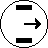
\includegraphics[angle=335,scale=.6]{pid/robot.pdf}};

\node[inner sep=0pt] (russell) at (axis cs:5.21,2.26)
    {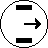
\includegraphics[angle=265,scale=.6]{pid/robot.pdf}};

\draw (axis cs:5,5) node[fill=white,draw,star,star points=5,star point ratio=.5]{};

\end{axis}
\end{tikzpicture}
\end{center}
\caption{Example trajectories for a proportional controller that moves
  a differential drive robot to a goal location.  The robot images
  indicate the starting positions for seven simulated navigation
  trials.}
\label{fig:diff_demo}
\end{figure}


Notice that, unlike the locomotive example, it wasn't necessary to
include integral or derivative terms in this controller.  They
weren't needed because we were able to set the speed of the
robot directly. This means we didn't need to worry as much about
overshooting the goal or applying too little force to reach it.  It
often makes sense to start with a pure proportional controller and add
integral or derivative terms if they prove necessary.

\section{Limitations of PID Controllers}

PID control is widely used because it is simple to implement and can
be applied in a wide range of situations.  We can use PID control even
when we don't have an accurate model of the system we are controlling.
In this chapter we used trial and error to develop a PID controller
for a simulated locomotive.  It wasn't necessary to understand the
physics involved: we didn't need to estimate frictional forces, we
didn't need an exact specification of the forces created by the
throttle.  We only needed to tune the three gain parameters until we
were satisfied with the performance.

The ad-hoc nature of PID control can also be seen as a disadvantage.
PID controllers tend to work well in practice, but they don't provide
any optimality guarantees.  In cases where we \emph{do} have an
accurate system model, it's possible to develop more principled
controllers that explicitly minimize a cost function related to the
quality of the solution.  This could allow us to create a controller
that reaches the goal in the minimum time or with minimal energy
expenditure.  Such controllers are beyond the scope of this book, but
the classic optimal controller is the \vocab{Linear Quadratic
  Regulator} or LQR.

More significantly, the kind of low-level control discussed in this
chapter is obviously not appropriate for complex control problems that
extend over longer periods of time.  A PID controller will not save
the day for the robot in Figure \ref{fig:maze}.  Problems like this
will require planning algorithms of the sort described in Chapter \ref{chap:planning}.

\begin{figure}[h!]
\begin{center}
\begin{tikzpicture}



\node[inner sep=0pt] (R) at (-3,-.2)
    {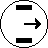
\includegraphics[angle=0,scale=.6]{pid/robot.pdf}};

%\draw ($(R) + (-.8, .8)$) node[draw,ellipse] {???};
\draw ($(R) + (-.5, .4)$) node[draw,ellipse,inner sep=0pt,minimum size=.6em] {};
\draw ($(R) + (-.35, .25)$) node[draw,ellipse,inner sep=0pt,minimum size=.3em] {};
\draw ($(R) + (-.8, 1)$) node [cloud, draw,cloud puffs=10,cloud puff arc=120, aspect=4, inner ysep=0em, minimum size=3em] {???};

% Star
\draw (3,.2) node[draw,star,star points=5,star point ratio=.5]{};

\node[inner sep=0pt] (M) at (0,0)
    {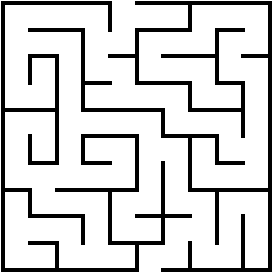
\includegraphics[angle=90,scale=1.1]{pid/figs/maze.pdf}};

\end{tikzpicture}

\end{center}
\caption{A control problem that can't be solved with the tools in this chapter.}
\label{fig:maze}
\end{figure}

\section{References and Further Reading}

\subsection{Closed-Loop Controllers}

Elements of the PID control model have been in place since the time of
the industrial revolution.  A history of the development of PID
control theory since 1900 is provided in \parencite{BENNETT200143}.
PID controllers are widely used in both robotics and industrial
automation, and as such, there is a huge literature on tuning and
implementing PID controllers. A recent 500-page reference can be found
in \parencite{johnson2006pid}.

A standard reference on the Linear Quadratic Regulator is
\parencite{anderson2007optimal}.

\subsection{General Robotics Resources}

There are a huge number of robotics textbooks and references.  I will
highlight a few here that are particularly notable and were useful in
the development of this book.

The most widely used artificial intelligence textbook is
\parencite{Russell2003}. While that book has a broader scope than just
robotics, many areas of AI are directly relevant to robotics
work. Another excellent general AI textbook is
\parencite{PooleMackworth17}.  This book has the advantage of being
available online at no cost: \url{https://artint.info/}.

\emph{Computational Principles of Mobile Robotics}
\parencite{dudek2010} is a robotics textbook that has a similar focus
to this work: it is targeted to computer scienists and focuses on
algorithmic issues in robotics.  An excellent open-access robotics
textbook is \parencite{correll2022introduction}.  The definitive work
on probalistic methods in robotics is \emph{Probalistic Robotics}
\parencite{thrun2005}.  An excellent, and authoritative, reference on
many topics in robotics is provided by the \emph{Springer Handbook of
  Robotics} \parencite{siciliano2008}.

%\section{Exercises}


\chapter{Coordinate Frames}

%-------------------------------------------------------------
\section{Introduction}
%-------------------------------------------------------------

A key requirement in robotics programming is keeping track of the
positions and velocities of objects in space.  For example, consider
the situation in Figure \ref{fig:robot_w_inset}.  This robot has been
programmed to find the blue teapot and report its position to a remote
user.  The robot's vision system has detected the teapot directly in
front of the camera at a distance of 1 meter.

\begin{figure}
\begin{center}
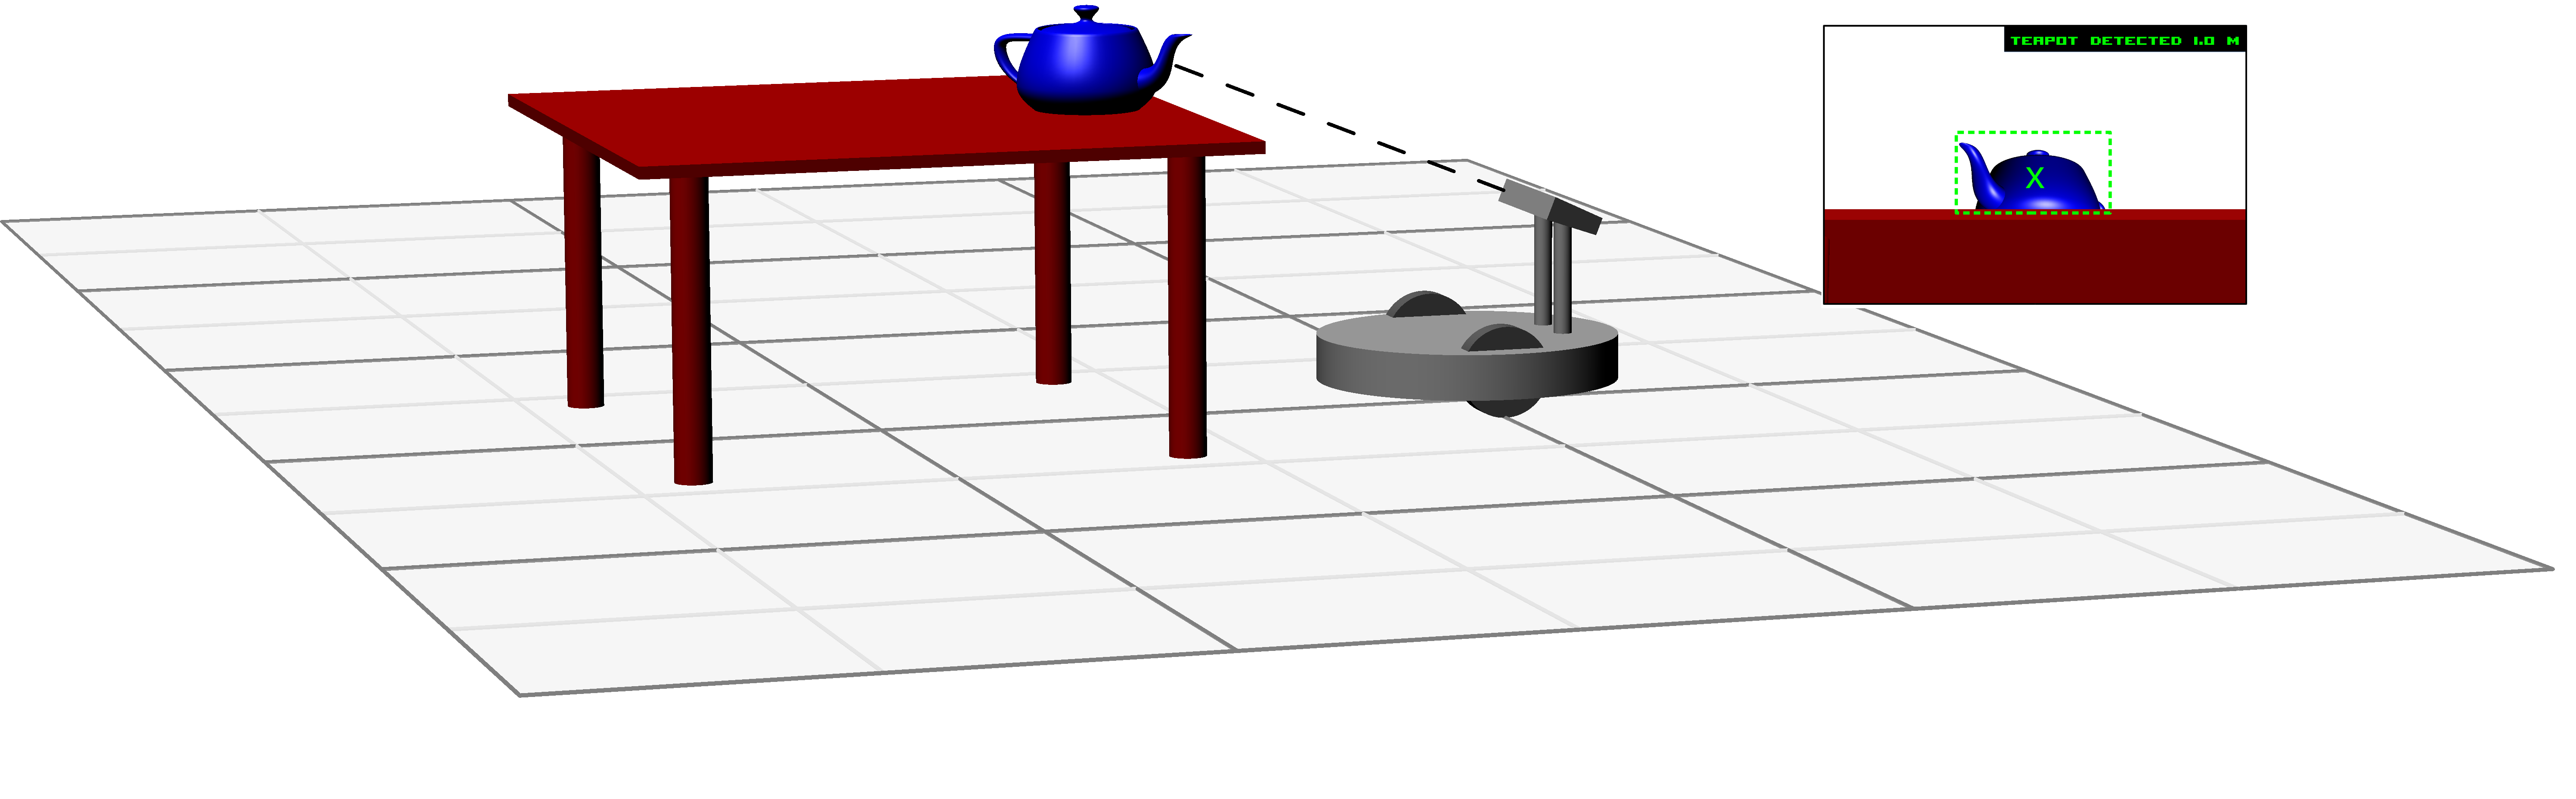
\includegraphics[]{frames/figs/robot_w_inset.png}
\end{center}
\caption{This robot has located a teapot and must report the location
  to a user.  The inset image shows the view from the robot's camera.}
\label{fig:robot_w_inset}
\end{figure}

In this situation it would not be very helpful to report to the user
that the teapot has been located \texttt{ONE METER IN FRONT OF MY
  CAMERA}.  Presumably, the user wants to know where \emph{in the
  room} the teapot is located. Providing this information requires us
to know each of the following:
\begin{enumerate}
\item{The position of the teapot relative to the camera. }
\item{The position and orientation of the camera relative to the base
  of the robot.}
\item{The position of the robot in the room.}
\end{enumerate}

Determining items 1 and 3 may be challenging problems on their own,
but for now, we will assume that we have access to this information.
The goal in this chapter is to develop a framework for representing
these relative locations and using that information to translate
coordinates from one frame of reference to another.  In this case,
from a frame of reference defined by the position of the camera
(\texttt{THE TEAPOT IS ONE METER IN FRONT OF MY CAMERA}), to a fixed
frame of reference defined relative to the room (\texttt{THE TEAPOT IS
  NEAR THE SOUTH-WEST CORNER OF THE ROOM}).

%-------------------------------------------------------------
\section{Conventions}
%-------------------------------------------------------------

As a first step we need to establish some conventions for describing
locations and orientations in three dimensions.

\begin{figure}
\begin{center}
\begin{tikzpicture}[x=.75cm,y=.75cm]
\draw[thick,->] (-.1,0) -- (3,0) node[anchor=north ] {$x$};
\draw[thick,->] (0,-.1) -- (0,3) node[anchor=east ] {$y$};
\draw[thick] (1.5,-1)  node[anchor=north ] {a}
;

    \foreach \x in {1, 2}
        \draw [](\x,1pt) -- (\x,-3pt)
            node[anchor=north] {$\x$};
    \foreach \y in {1, 2}
        \draw (1pt,\y) -- (-3pt,\y) node[anchor=east] {$\y$};

\end{tikzpicture}
\hspace{.75in}
\begin{tikzpicture}[x=.75cm,y=.75cm]
\draw[thick,->] (-.1,3) -- (3,3) node[anchor=south ] {$x$};
\draw[thick,->] (0,3.1) -- (0,0) node[anchor=east ] {$y$};
\draw[thick] (1.5,-1)  node[anchor=north ] {b};


    \foreach \x in {1, 2}
        \draw []($(\x,3pt)+(0,3)$) node[anchor=south] {$\x$} -- ($(\x, -1pt) +(0,3)$);
    \foreach \y in {2,1}
        \draw (1pt,3-\y) -- (-3pt,3-\y) node[anchor=east] {$\y$};

\end{tikzpicture}
\end{center}
\caption{There are several ways we can draw two-dimensional coordinate systems.  a.  The origin is drawn in the lower-left corner. b. the origin is drawn in the upper-left.}
\label{fig:two_d_coordinates}
\end{figure}


You certainly have experience working with two-dimensional coordinate
systems like the one illustrated in Figure
\ref{fig:two_d_coordinates}a.  This figure follows the common
convention of placing the origin is at the lower-left with the
positive x-axis draw horizontally and the positive y-axis drawn
vertically.

It is possible to draw this coordinate system differently. For
example, the convention when working with coordinates on a computer
screen is to place the origin at the upper-left corner as shown in
Figure \ref{fig:two_d_coordinates}b.

In a sense, Figures \ref{fig:two_d_coordinates}a and
\ref{fig:two_d_coordinates}b are the same coordinate system drawn in
two different ways.  You can imagine picking up the axes in Figure
\ref{fig:two_d_coordinates}a, flipping them over and placing them back
on top of the axes in Figure \ref{fig:two_d_coordinates}b so that the
axes are aligned.


\begin{figure}
\begin{center}

\tdplotsetmaincoords{76}{243}
\begin{tikzpicture}[tdplot_main_coords]

\draw[thick,->] node[inner sep=0pt] (hand) at  (-.3,-.2,0) {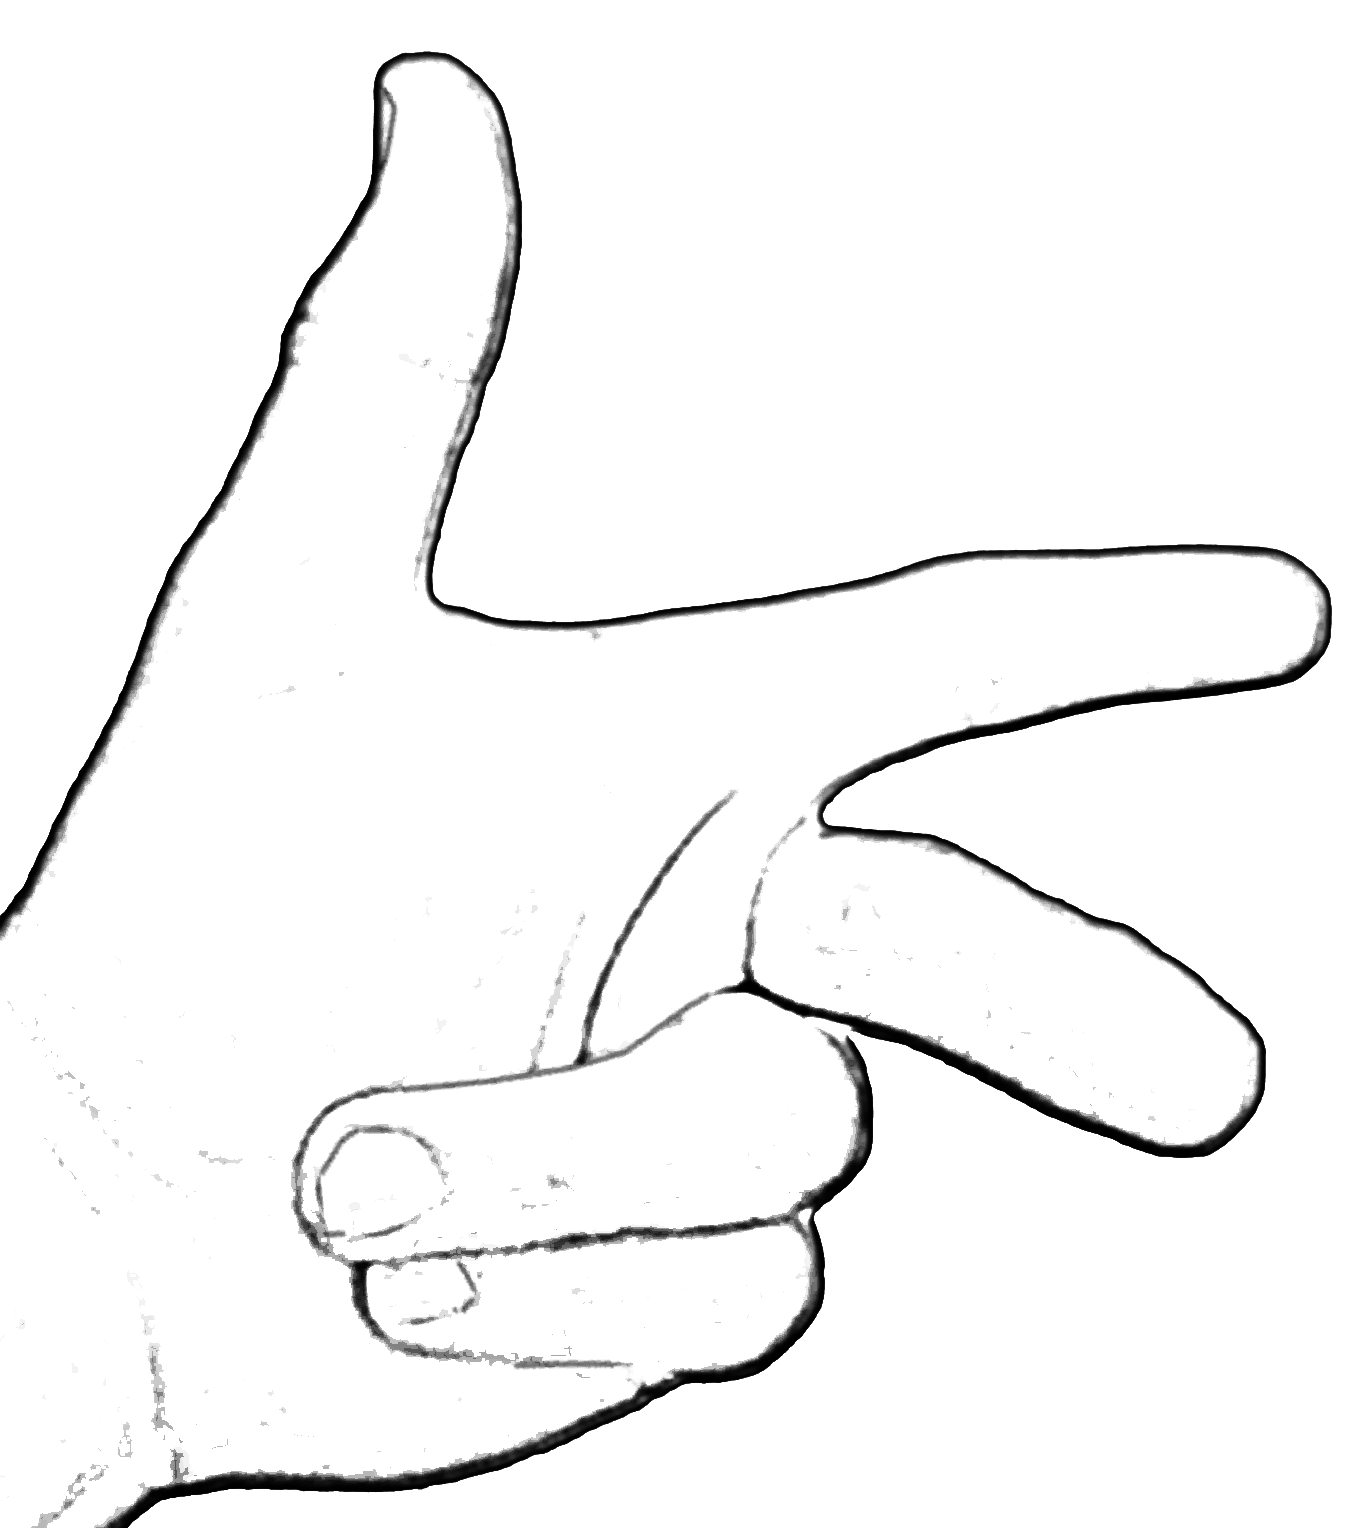
\includegraphics[width=.15\textwidth]{frames/figs/left_hand_gray.png}};
%\draw[thick,->] (-2.7,0,0) -- (-3.95,0,0) node[anchor=north east]{$y$};
%\draw[thick,->] (0,-1.55,0) -- (0,-2.8,0) node[anchor=north west]{$x$};
%\draw[thick,->] (0,0,1.1) -- (0,0,2.35) node[anchor=south]{$z$};
\draw[thick,->] (0,0,0) -- (-3.,0,0) node[anchor=north east]{$y$};
\draw[thick,->] (0,0,0) -- (0,-3.,0) node[anchor=north west]{$x$};
\draw[thick,->] (0,0,0) -- (0,0,3.) node[anchor=south]{$z$};
\end{tikzpicture}
\hspace{1in}
\tdplotsetmaincoords{74}{210}
\begin{tikzpicture}[tdplot_main_coords]

\draw[thick,->] node[inner sep=0pt] (hand) at  (.3,0,-.1) {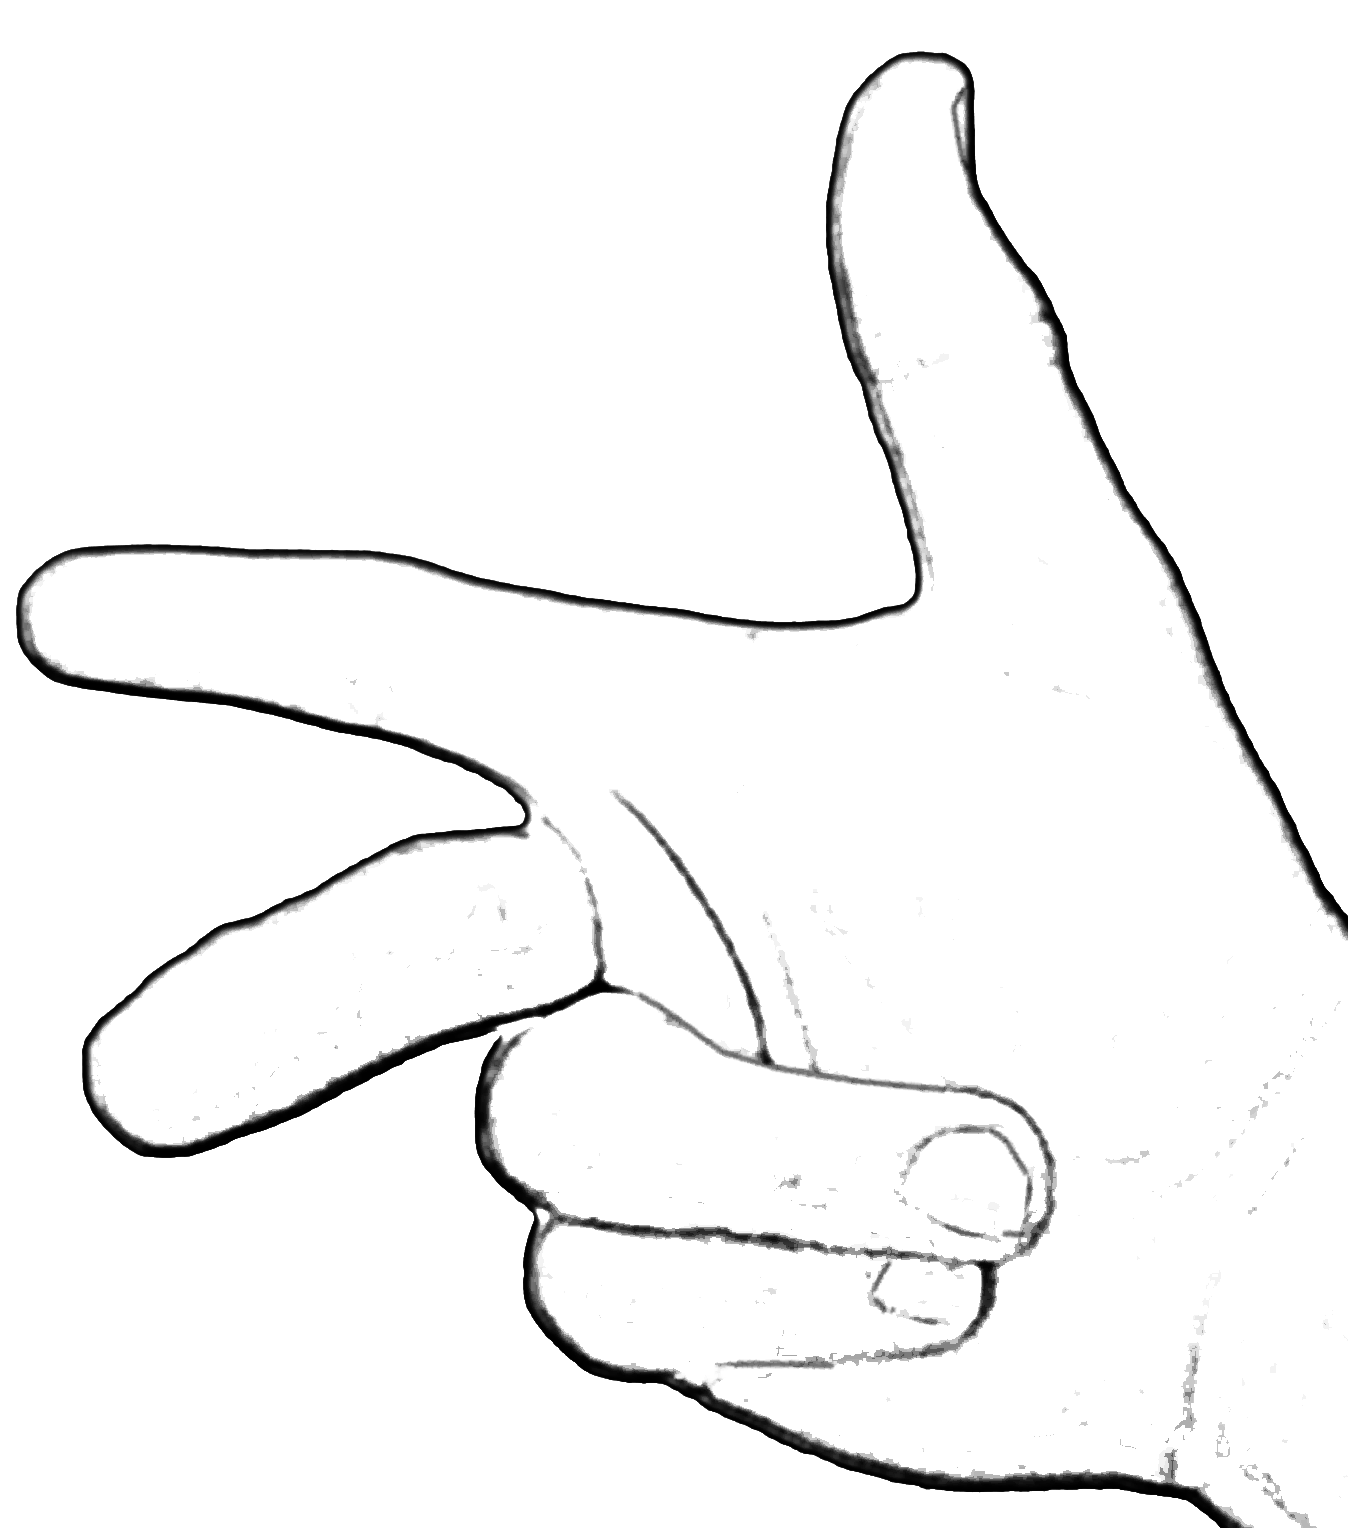
\includegraphics[width=.15\textwidth]{frames/figs/right_hand_gray.png}};
%\draw[thick,->] (1.45,0,0) -- (2.95,0,0) node[anchor=north east]{$x$};
%\draw[thick,->] (0,2.25,0) -- (0,3.5,0) node[anchor=north west]{$y$};
%\draw[thick,->] (0,0,1.2) -- (0,0,2.45) node[anchor=south]{$z$};
\draw[thick,->] (0,0,0) -- (3,0,0) node[anchor=north east]{$x$};
\draw[thick,->] (0,0,0) -- (0,3,0) node[anchor=north west]{$y$};
\draw[thick,->] (0,0,0) -- (0,0,3) node[anchor=south]{$z$};
\end{tikzpicture}
\end{center}
\caption{Left and right-handed coordinate systems.}
\label{fig:left_right_coordinates}
\end{figure}


The situation is different in three dimensions.  Depending on how the
axes are arranged we can end up with one of two fundamentally
incompatible coordinate systems as illustrated in Figure
\ref{fig:left_right_coordinates}.  The coordinate system on the left
is referred to as a \vocab{left-handed coordinate system}, while the one on
the right is a \vocab{right-handed coordinate system}.  In a right-handed
coordinate system we determine the direction of the $z$-axis by aiming
the pointer finger of the right hand along the positive $x$-axis and
curling our palm toward the positive $y$-axis.  The thumb will then
point in the direction of positive $z$.  For a left-handed coordinate
system we follow the same procedure using the left hand.

There is no way to rotate these two coordinate systems so that they
align.  They represent two incompatible ways of representing
three-dimensional coordinates.  This means that whenever we provide
coordinates in three dimensions we must specify whether we are using a
left-handed or right-handed system.  There is no universal convention
for which should be used, but right-handed systems are more common in
robotics.  All of the examples in this book will assume right-handed
coordinate systems.

%x forward, y left, z up
\begin{figure}
\begin{center}
\tdplotsetmaincoords{60}{110}
\begin{tikzpicture}[tdplot_main_coords]

\draw[thick,->] node[inner sep=0pt] (hand) at  (0,.2,0) {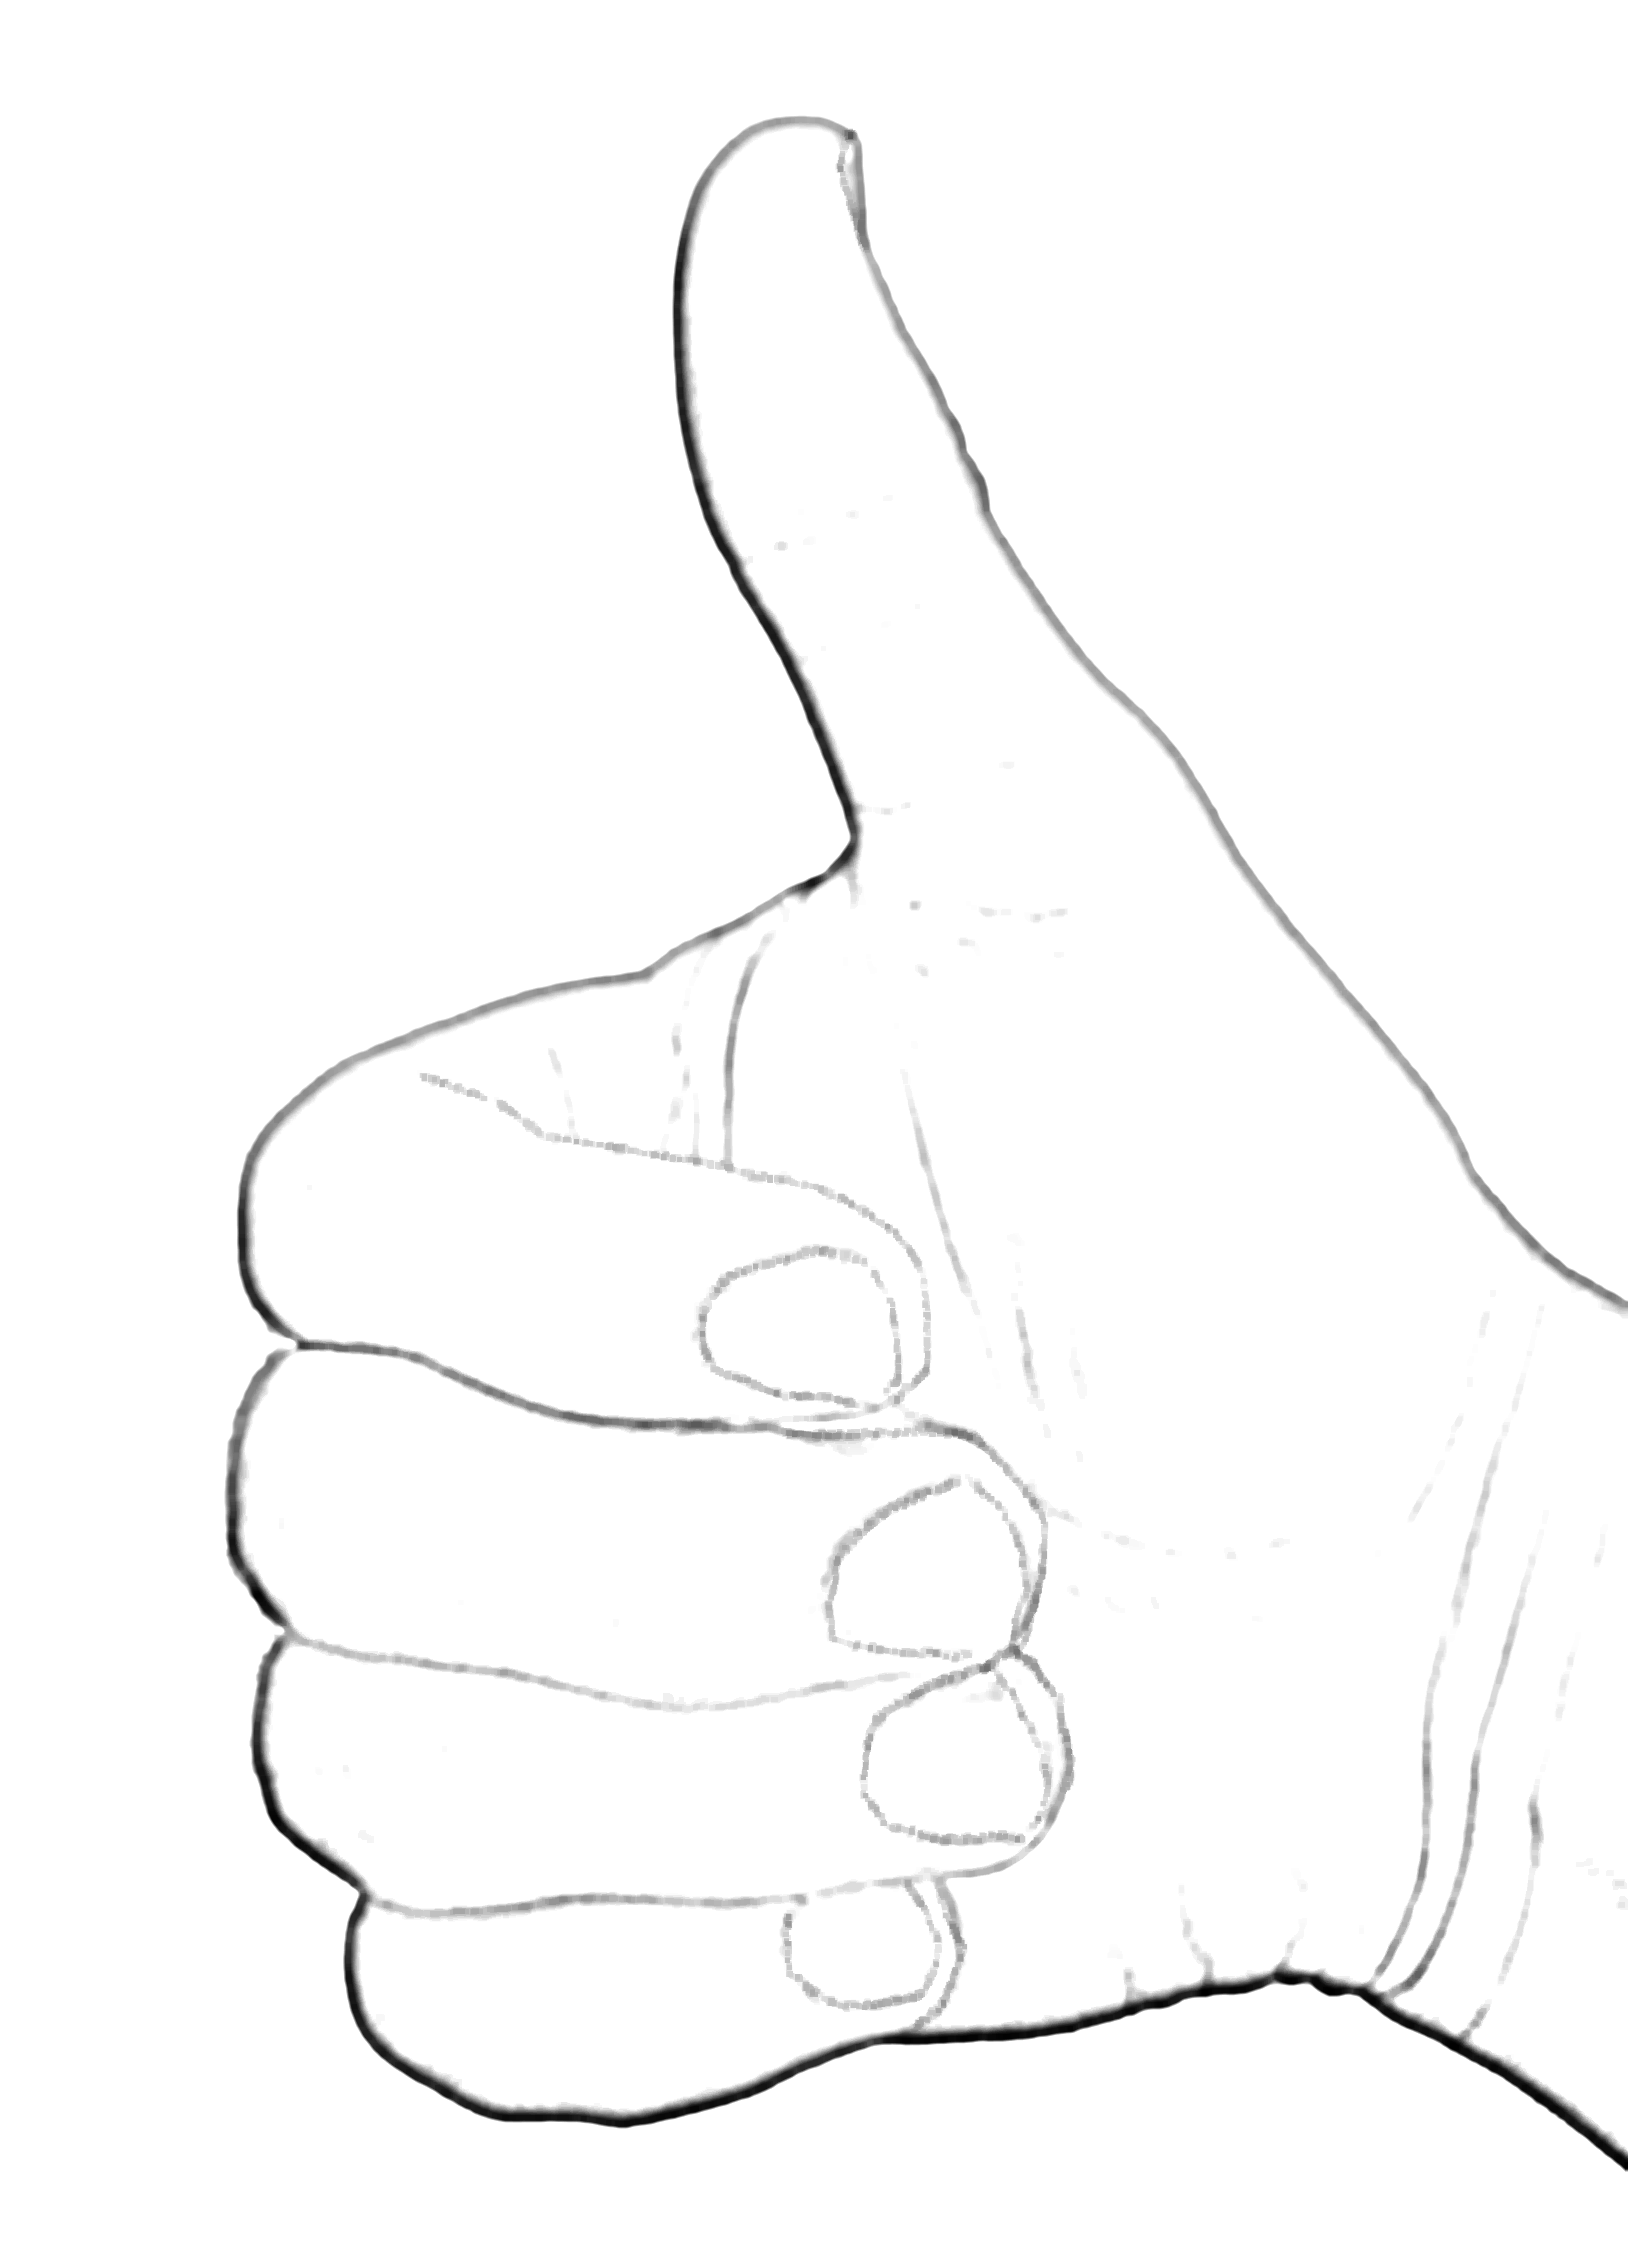
\includegraphics[width=.15\textwidth]{frames/figs/right_hand_rotation_small.png}};

\tdplotdrawarc[thick,->,color=blue]{(0,0,1.7)}{0.5}{50}{340}{anchor=west,color=black}{$\;\;+\Theta$}

\draw[thick,->] (0,0,-.06) -- (0,0,2.45) node[anchor=south]{$z$};
\draw[thick] (0,0,-1.3) -- (0,0,-2) node[anchor=south]{};


\end{tikzpicture}
\end{center}
\caption{Right-hand rule for determining the direction of positive
  rotations around an axis.}
\label{fig:right_hand_rotation}
\end{figure}


We also need to establish a convention for describing the direction of
a rotation.  Again, we will follow a right-hand rule.  To determine
the direction of positive rotation around a particular axis we point
the thumb of the right hand along the axis in question.  The fingers
will then curl around the axis in the direction of positive rotation.
This is illustrated in Figure \ref{fig:right_hand_rotation}.



%-------------------------------------------------------------
\section{Poses and Coordinate Frames}
%-------------------------------------------------------------

%http://wiki.ros.org/tf/Overview/Transformations

The position and orientation of an object in space is referred to as
its \vocab{pose}\index{pose}.  Any description of an object's pose
must always be made in relation to some to some \vocab{coordinate
  frame}.  It isn't helpful to know that my teapot is at position (-2,
2.2, 1.6) unless I know where (0, 0, 0) is and which directions the
three axes are pointing.

\begin{figure}
  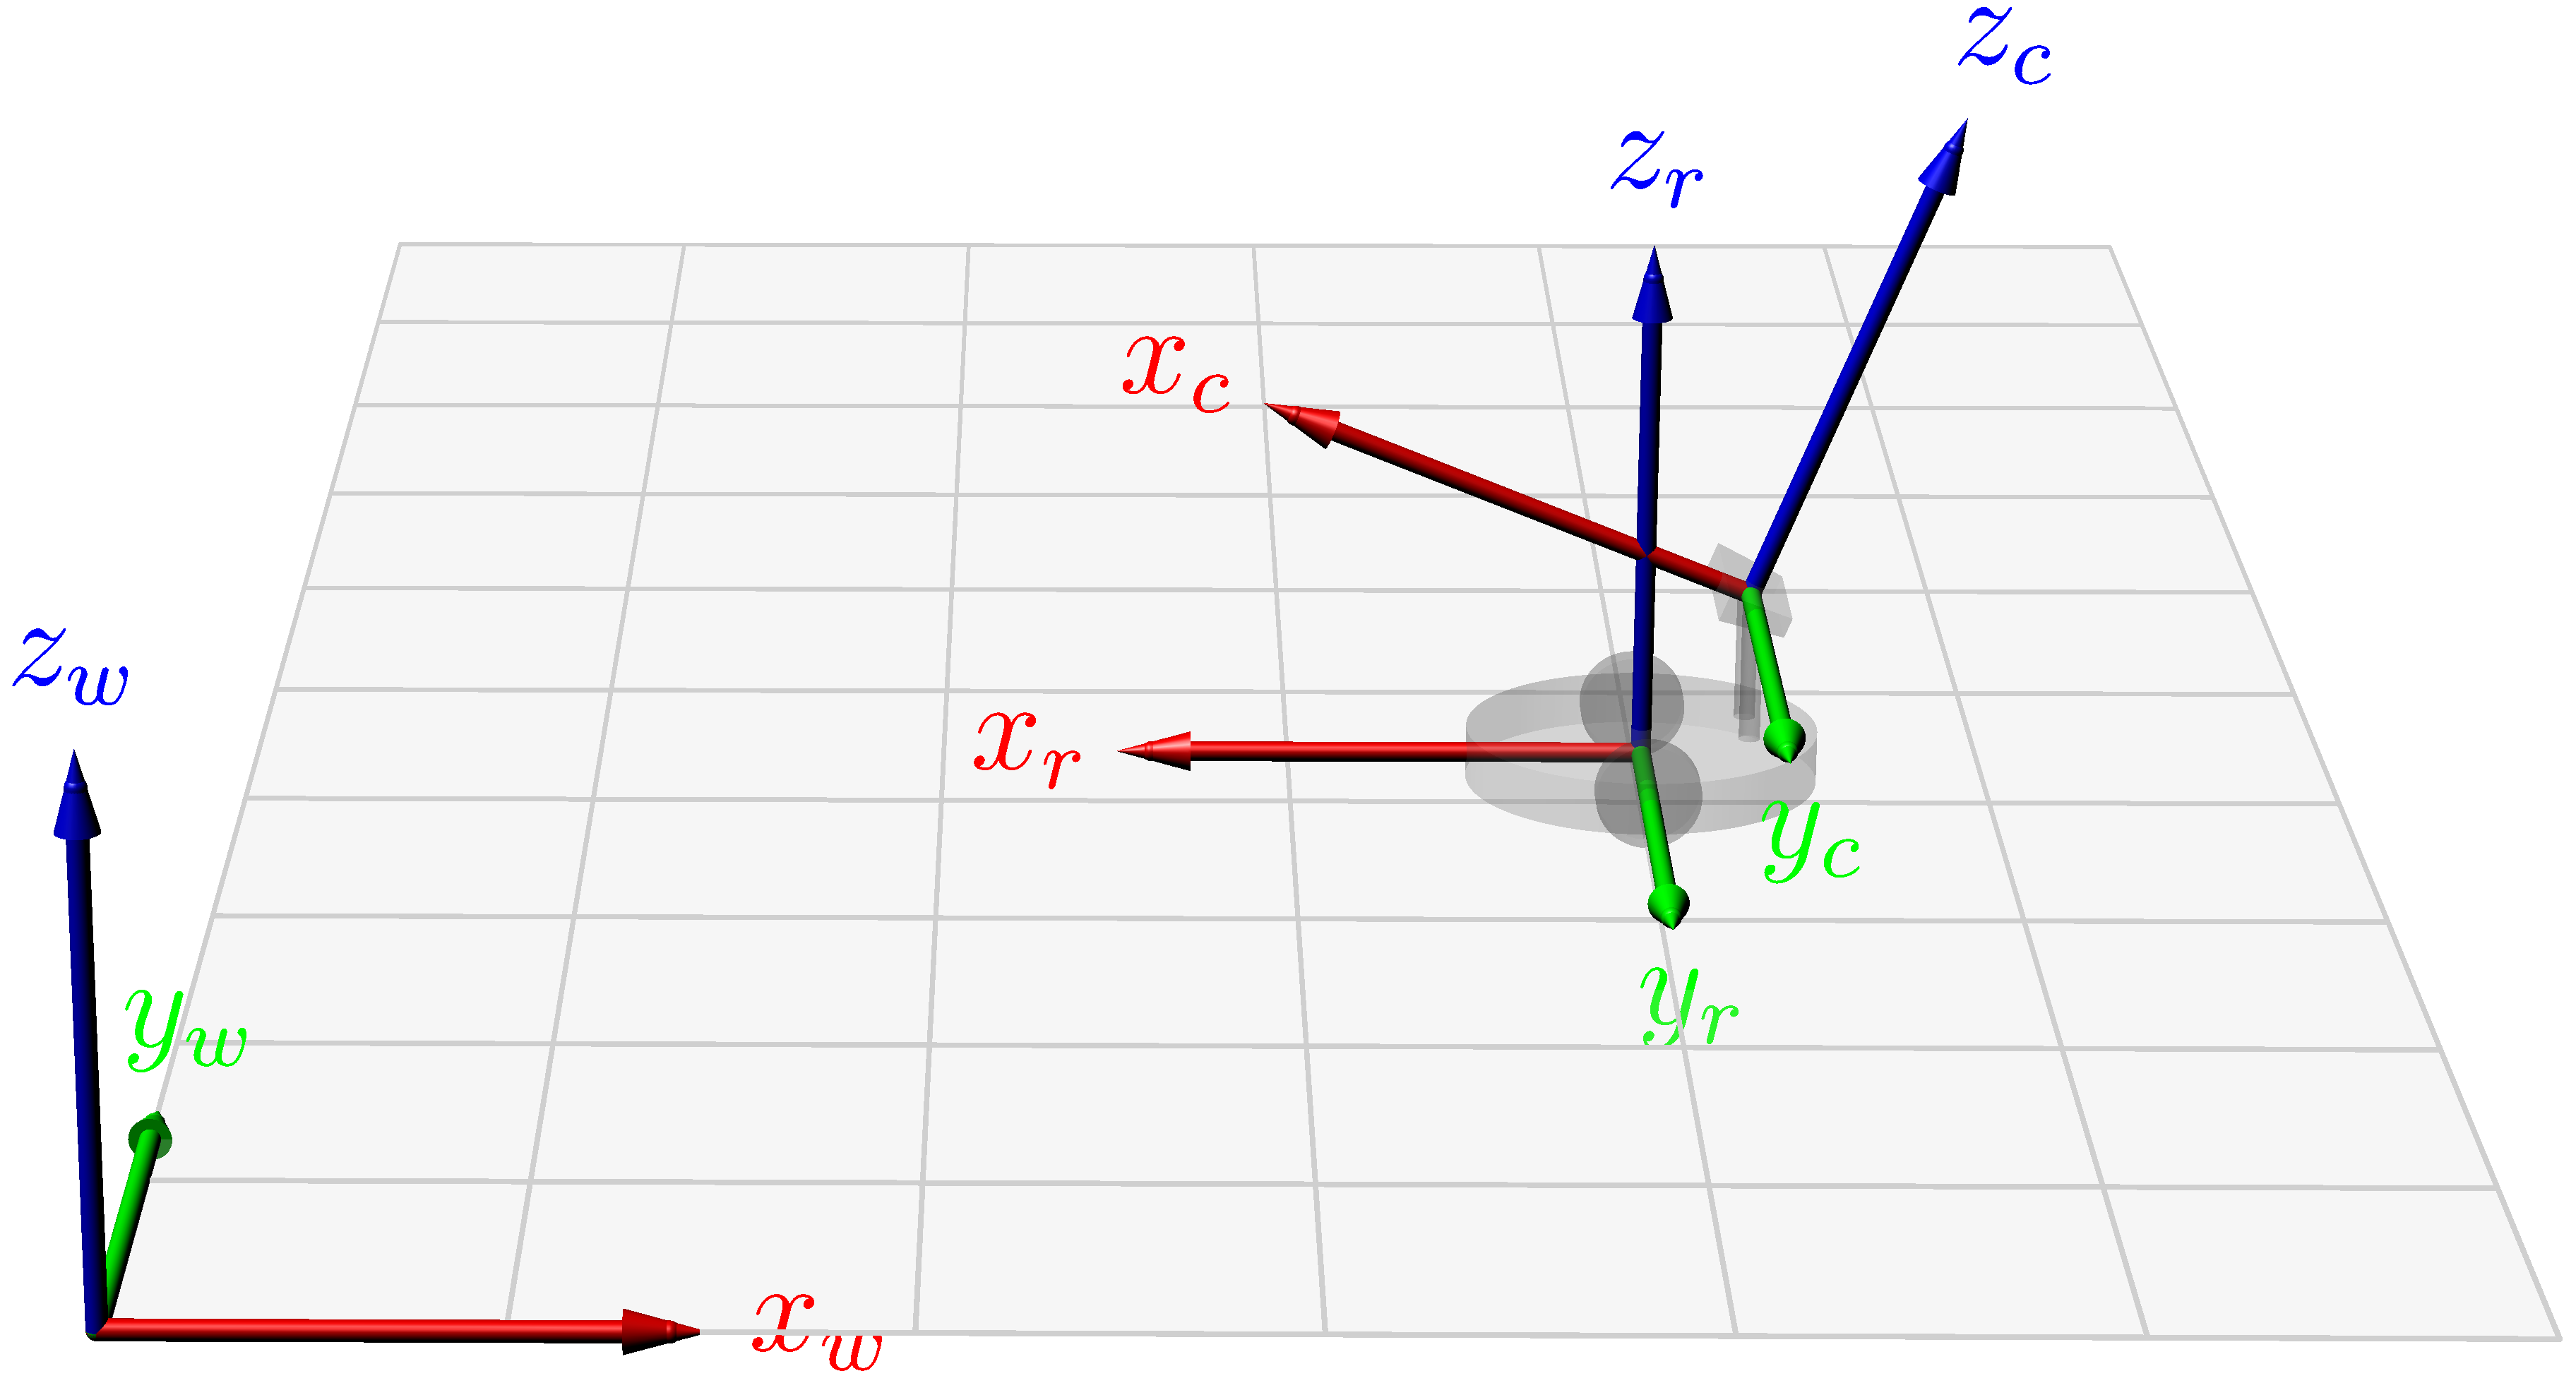
\includegraphics[]{frames/figs/frames.png}
  \hspace{.5in}
\begin{tikzpicture}
\node[circle,draw](z){$w$}
  child[missing]{}
  child{
    node[circle,draw]{$r$} child{node[circle,draw] {$c$}} };
\end{tikzpicture}

\caption{Left: three coordinate frames from the teapot scenario
  illustrated in Figure \ref{fig:robot_w_inset}.  Right: tree
  representing the relationship between the three coordinate frames.}

\label{fig:frames}
\end{figure}

In robotics, it is often convenient to keep track of multiple
coordinate frames. Figure \ref{fig:frames}  illustrates three potentially useful
coordinate frames related to the teapot scenario described above.  The
``world'' coordinate frame is indicated with the subscript $w$.  This
coordinate frame is fixed at a known location in space and assumed not
to move over time.  The ``robot'' coordinate frame is indicated with
the subscript $r$.  We can envision this coordinate frame as being
attached to the base of the robot so that the origin of the frame
moves as the robot moves.  In other words, the robot is always located
at (0, 0, 0) in its own coordinate frame.  Similarly, the ``camera''
coordinate frame is attached to the camera.

This figure follows the common convention of drawing the $x$-axis in
red, the $y$-axis in green and the $z$-axis in blue.  In the case of
robots (and many other objects) we have a natural notion of directions
corresponding to ``forward'', ``left'' and ``up''.  Throughout this
book these will correspond to positive $x$, positive $y$ and positive
$z$ respectively.

We can organize these three coordinate frames into a tree structure
with the ``world'' coordinate frame as the root.  Each edge in the
tree represents the pose of a particular coordinate frame relative to
its parent.  Ideally, this tree structure should mirror the physical
connections between the objects involved.  In this case it makes sense
to describe the pose of the camera in the robot's coordinate frame,
because the two are physically attached and the camera is constrained
to move along with the robot.  When the robot moves, it is only
necessary to update the pose of the robot coordinate frame.  The
camera remains stationary relative to the robot.

%% Restricting our graph structure to be a tree prevents ambiguity.  If
%% there were more than one path from the root to a particular node then
%% it would require extra effort to make sure that the two paths are in
%% agreement.

Assuming a connected tree, it will be possible to translate a point
between any two coordinate frames.  For example, given the coordinates
of the teapot in the camera coordinate frame, we can determine its
coordinates in the robot coordinate frame, and then in the room
coordinate frame.  In order to accomplish this we need to specify how
poses are represented.  We also need a mechanism for converting from
parent to child coordinate frames and vise-versa.



\subsection{Translations}
\label{sec:tranlations}
Recall that the pose of an object (or a coordinate frame) includes
both its position and orientation relative to the parent coordinate
frame.  Representing the position is straightforward.  Three numbers
may be used to represent a translation of the object along each of the
three axes of the parent coordinate frame.


\begin{figure}
\begin{center}
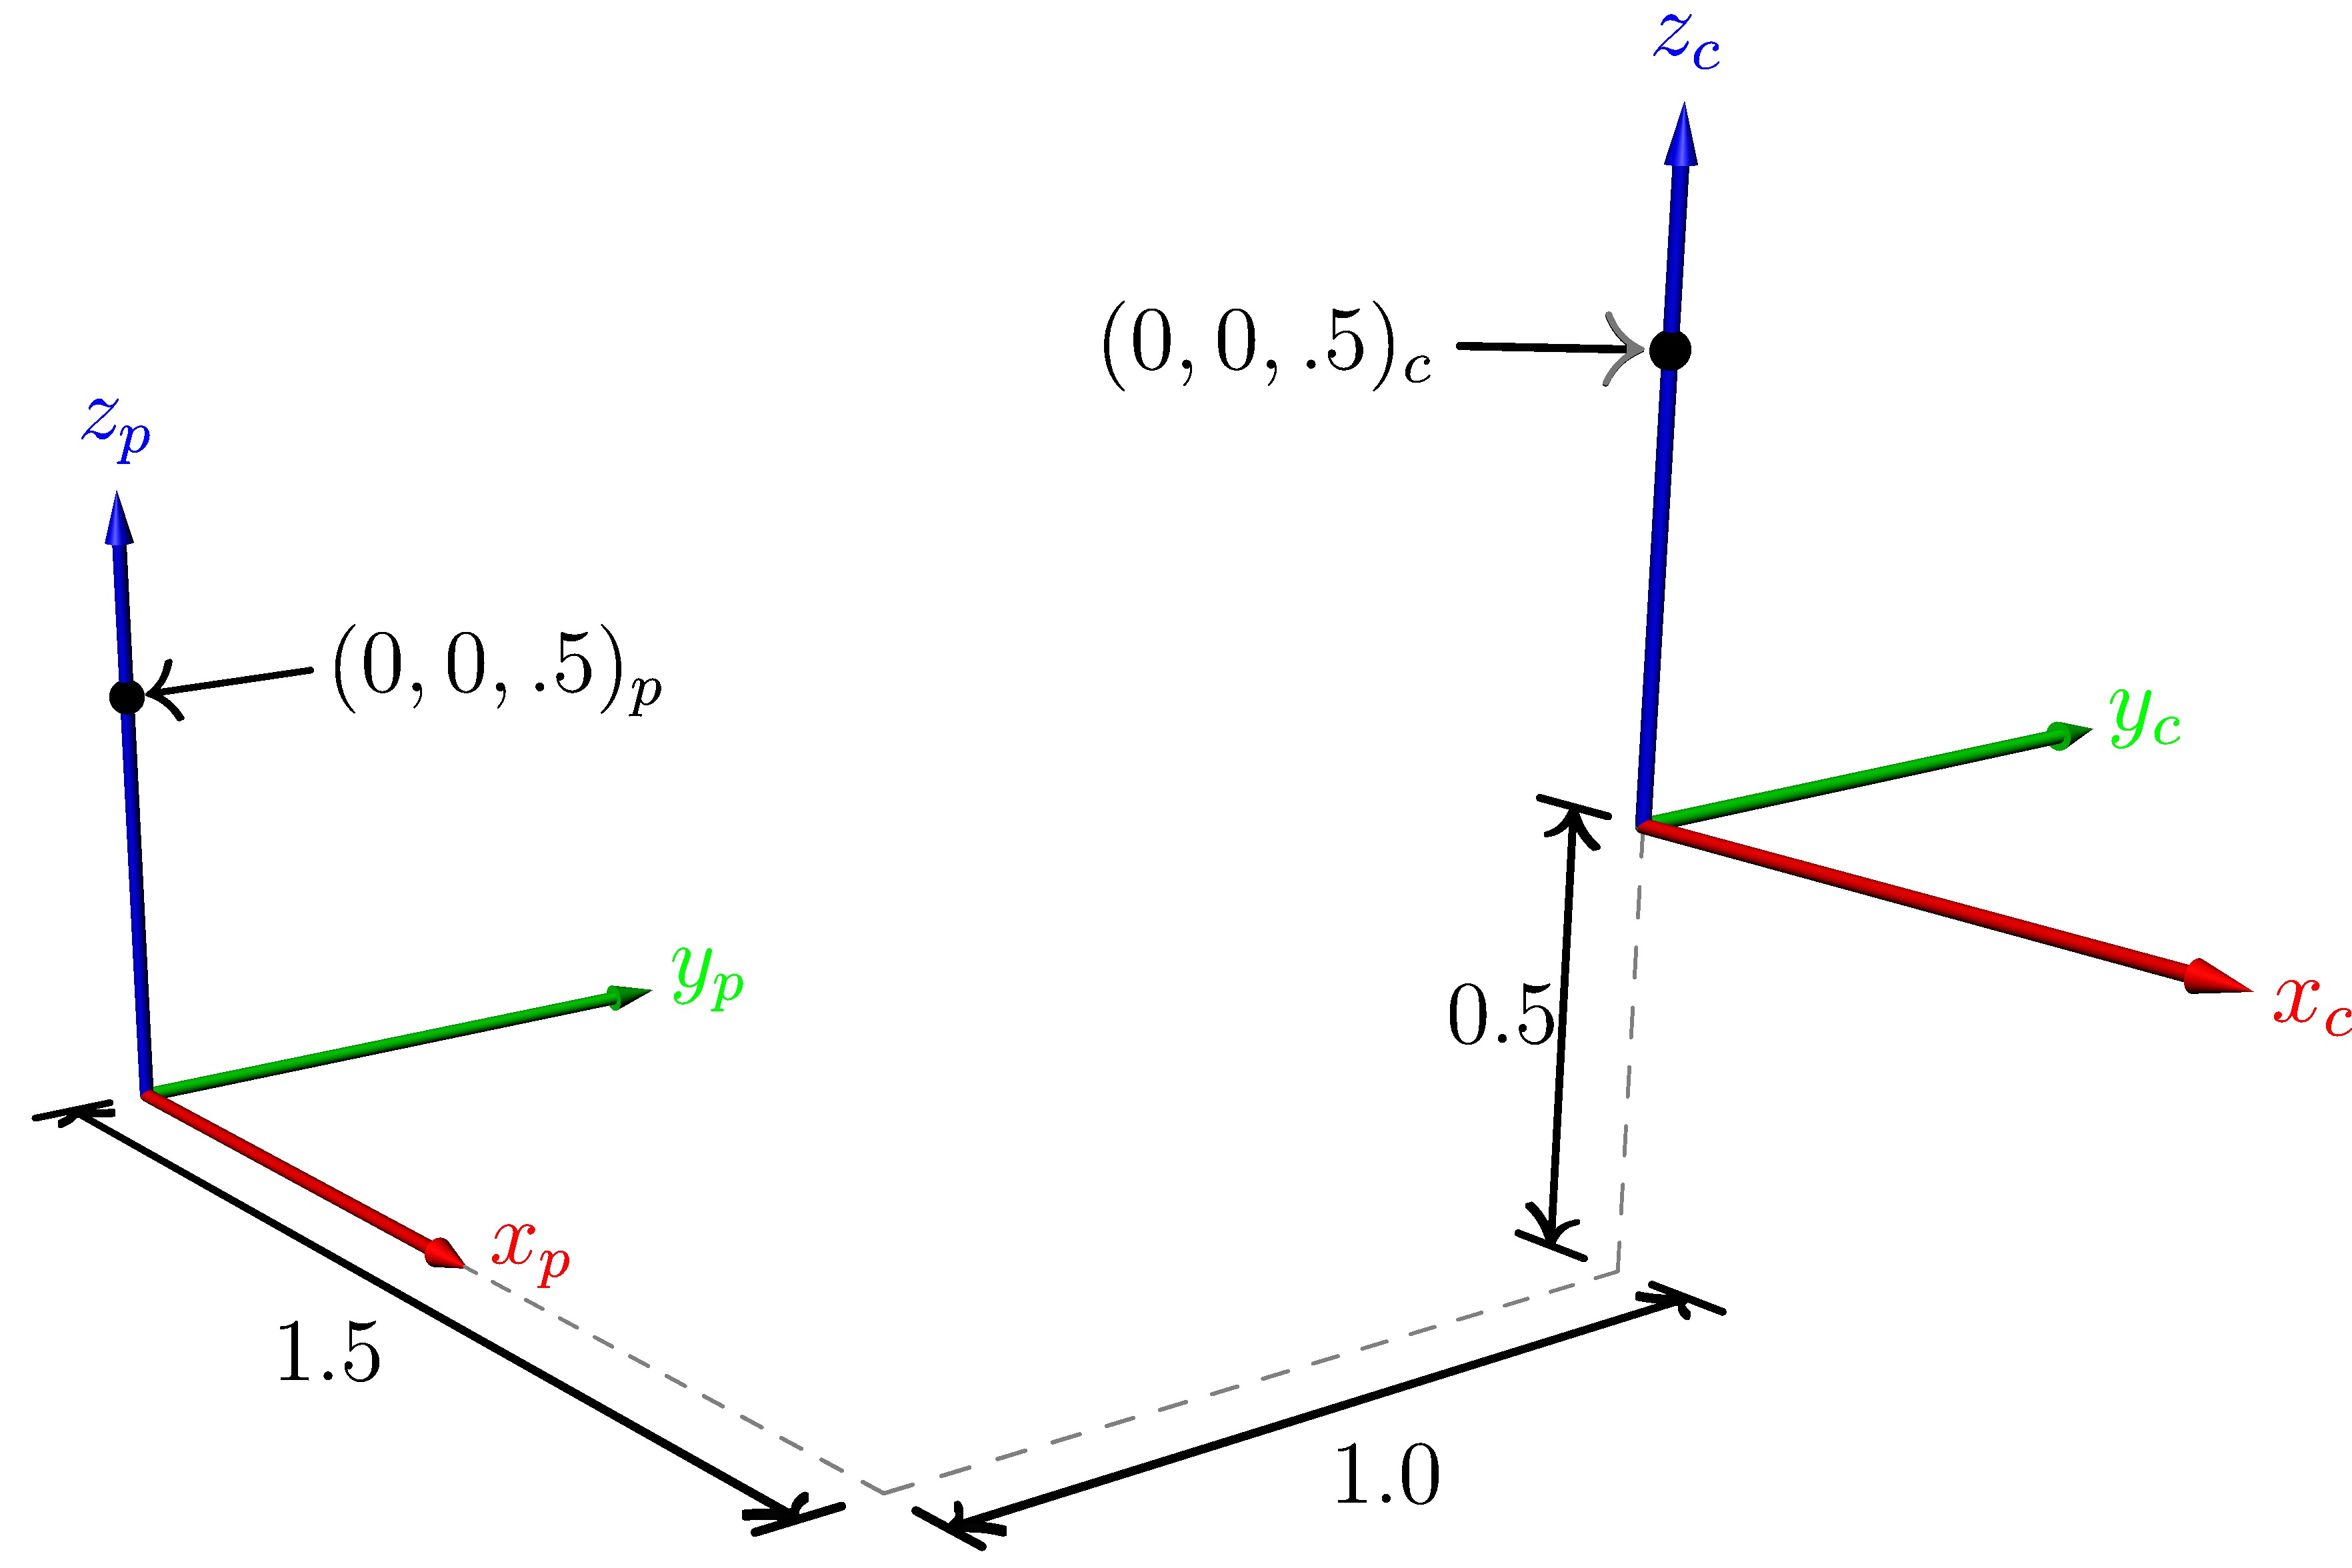
\includegraphics[]{frames/figs/translation.png}
\end{center}
\caption{Two coordinate frames separated by a simple translation. The
  parent frame is labeled $p$, the child frame is labeled $c$. }
\label{fig:translation}
\end{figure}

Figure \ref{fig:translation} shows two coordinate frames separated by
a simple translation.  In this example, the child coordinate frame
is located at position (1.5, 1.0, .5) in the parent coordinate
frame.

We will use subscripts to indicate the coordinate
frame associated with a point or pose.  For example,
$(0, 0, .5)_c$, refers to the point $(0, 0, .5)$
in the child coordinate frame.

When coordinate frames are separated by a pure translation
transforming points between frames is straightforward: we only need to
add or subtract the three coordinate offsets.  For example, the point
$(0, 0, .5)_c$ is located at $(0 + 1.5, 0 + 1.0, .5 + .5) =
(1.5, 1.0, .5)$ in the parent coordinate frame.  Moving from the
parent to the child requies us to subtract instead of add: $(0, 0,
.5)_p$ is located at $(-1.5, -1.0, 0)$ in the child frame.


\subsection{Euler Angles}
\label{sec:euler}

Specifying orientation in three dimensions is more complicated than
specifying position.  There are several approaches, each with its own
strengths and weaknesses.  \vocab{Euler angles} are probably the most
intuitive representation. Figure \ref{fig:euler} illustrates the basic
idea.  Orientation is expressed as a sequence of three rotations
around the three coordinate axes.  These three rotations are
traditionally referred to as \vocab{roll}, \vocab{pitch} and \vocab{yaw}.

\begin{figure}
\begin{center}
\tdplotsetmaincoords{60}{130}
\begin{tikzpicture}[tdplot_main_coords]

\draw[thick,->] node[inner sep=0pt] (hand) at  (0,0,0) {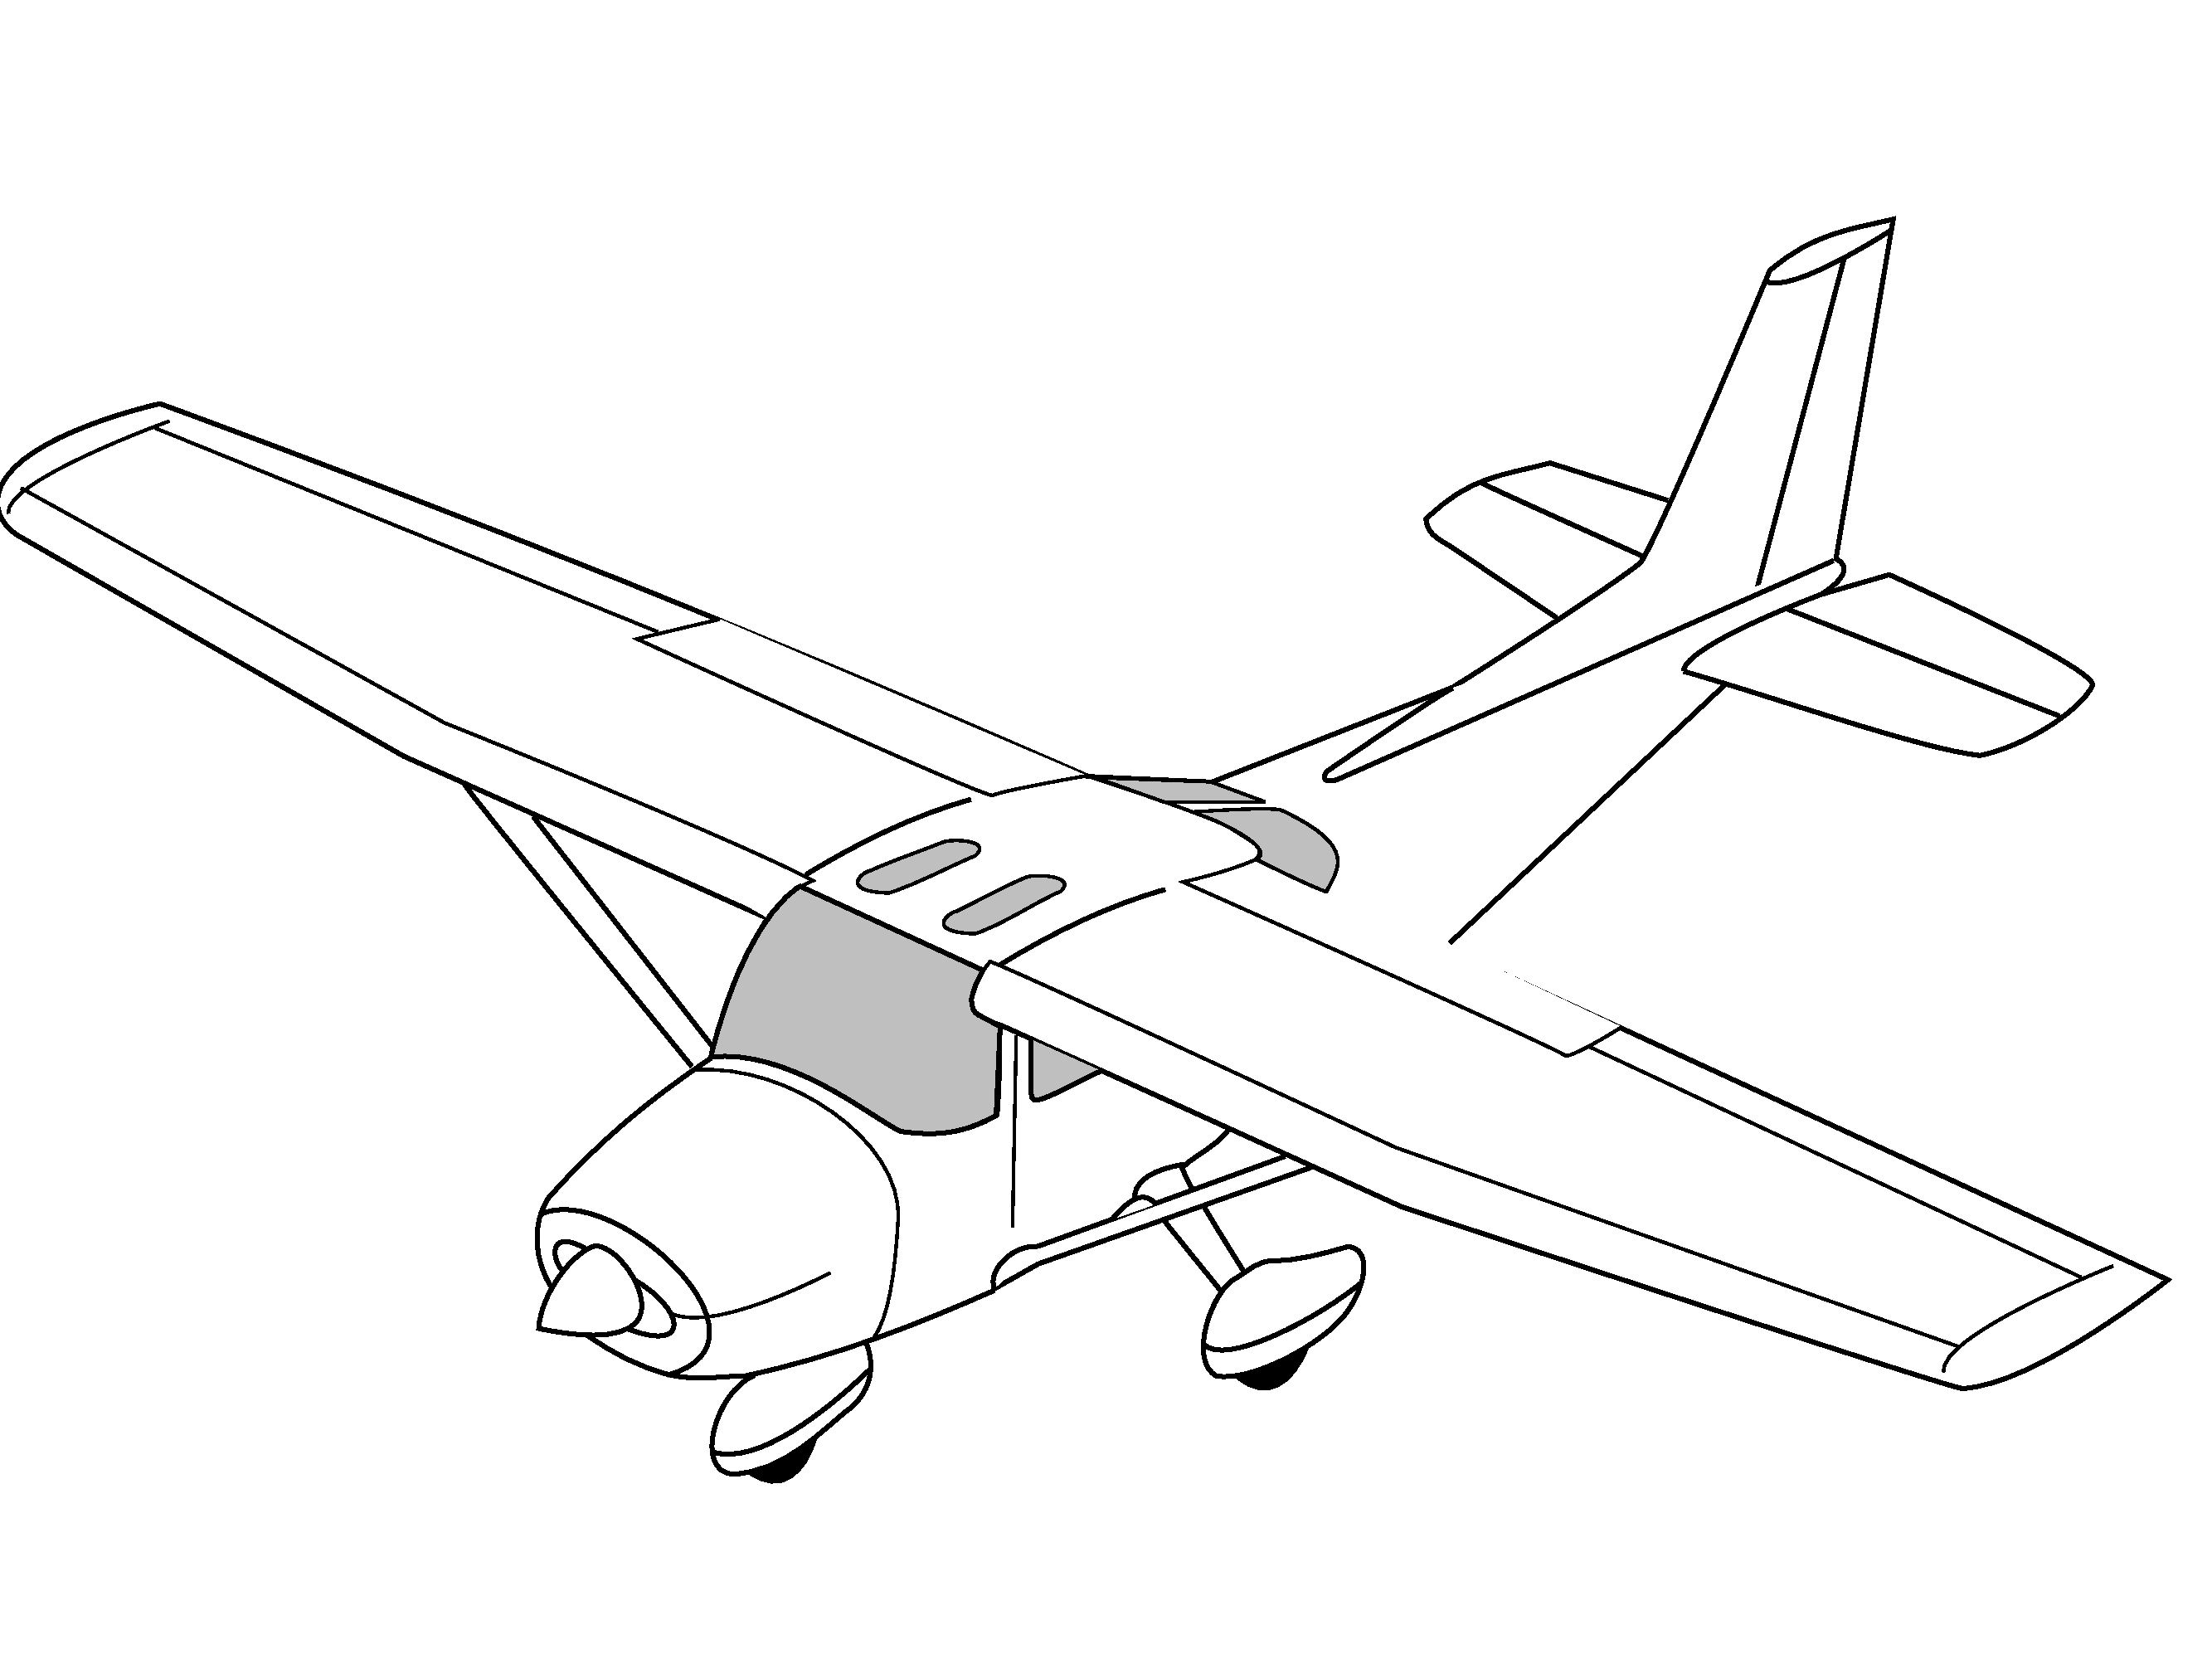
\includegraphics[width=.15\textwidth]{frames/figs/airplane-297578.pdf}};

\draw[thick,->] (0,0,0) -- (3,0,0) node[anchor=north east]{$x$};
\draw[thick,->] (0,0,0) -- (0,3,0) node[anchor=north west]{$y$};
\draw[thick,->] (0,0,0) -- (0,0,3) node[anchor=south]{$z$};

\tdplotdrawarc[thick,->,color=blue,inner sep=10]{(0,0,1.7)}{0.3}{50}{340}{anchor=west,color=black}{yaw}

\tdplotsetrotatedcoords{ 0 }{ 90 }{ 0 }
\tdplotdrawarc[thick,->,color=blue,tdplot_rotated_coords,inner sep=10]{(0,0,1.7)}{0.3}{50}{340}{anchor=east,color=black}{roll}

\tdplotsetrotatedcoords{90  }{ 90}{ 0 }
\tdplotdrawarc[thick,->,color=blue,tdplot_rotated_coords,inner sep=10]{(0,0,1.7)}{0.3}{50}{340}{anchor=west,color=black}{pitch}
\end{tikzpicture}


\end{center}
\caption{Euler angles.}
\label{fig:euler}
\end{figure}


When working with Euler angles it is necessary to specify the order
that the rotations will be applied: a $90^o$ rotation around the
$x$-axis followed by a $90^o$ rotation around the $y$-axis does
\emph{not} result in the same orientaion as the same rotations applied
in the opposite order.  There are, in fact, \emph{twelve} valid
rotation orderings: xyz, yzx, zxy, xzy, zyx, yxz, zxz, xyx, yzy, zyz,
xzx, and yxy.


\begin{figure}
\begin{center}

\begin{tikzpicture}
\node[inner sep=0pt] (e0) at (0,5.0)
    {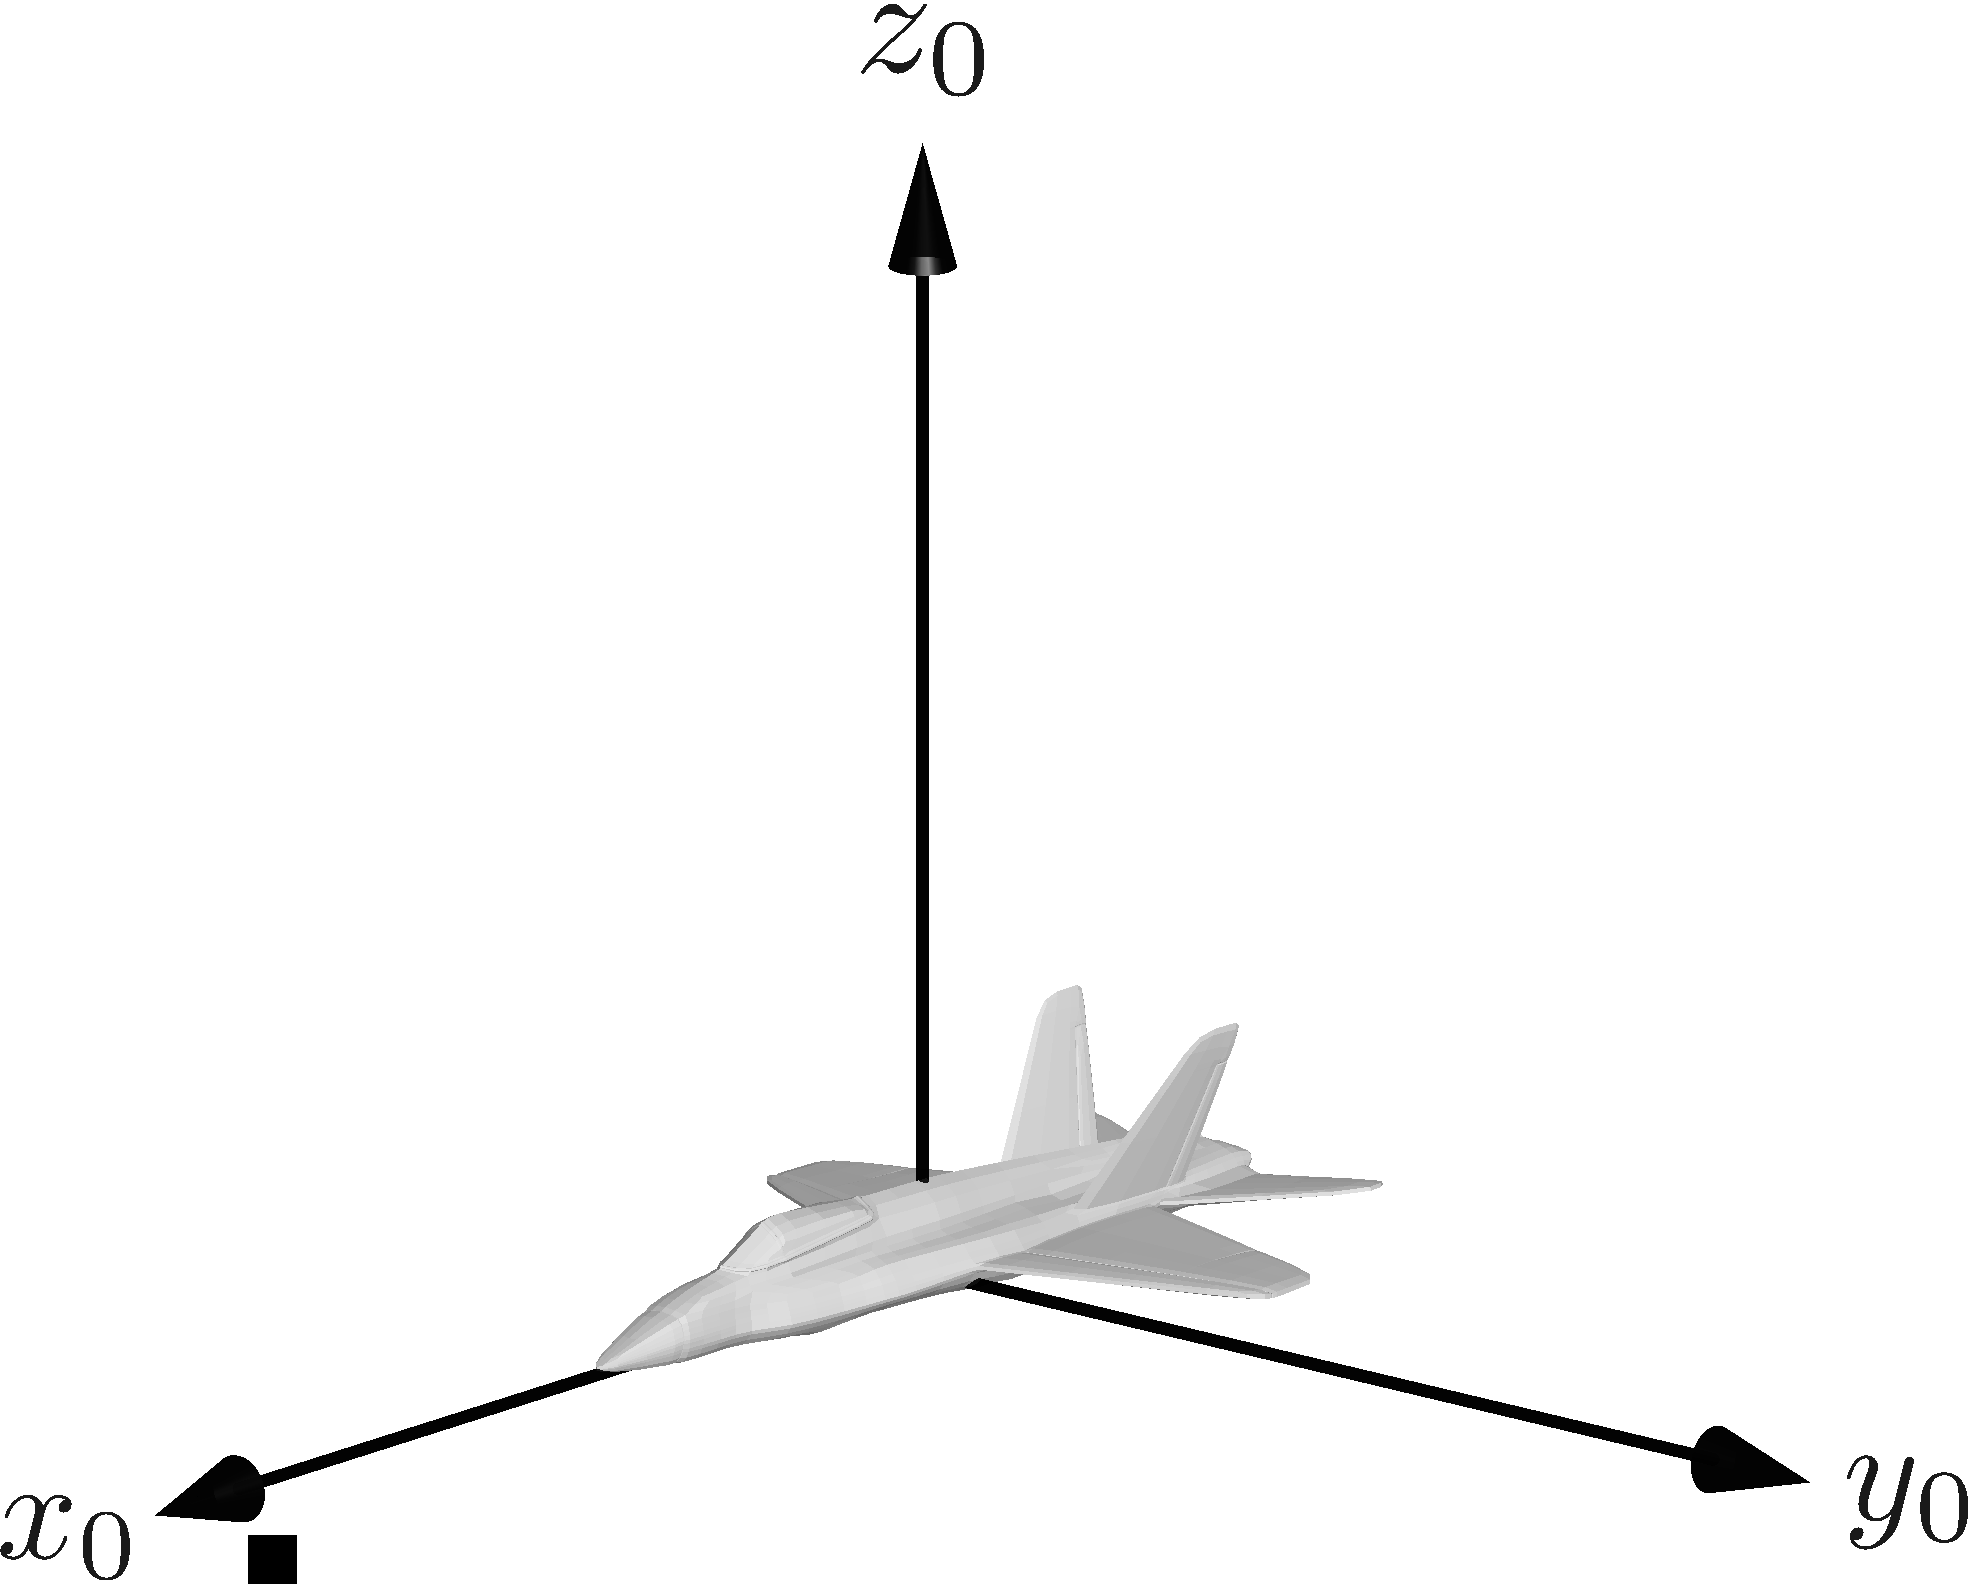
\includegraphics{frames/figs/euler_static_0.png}};
\node[inner sep=0pt] (e1) at (6.0,5.0)
    {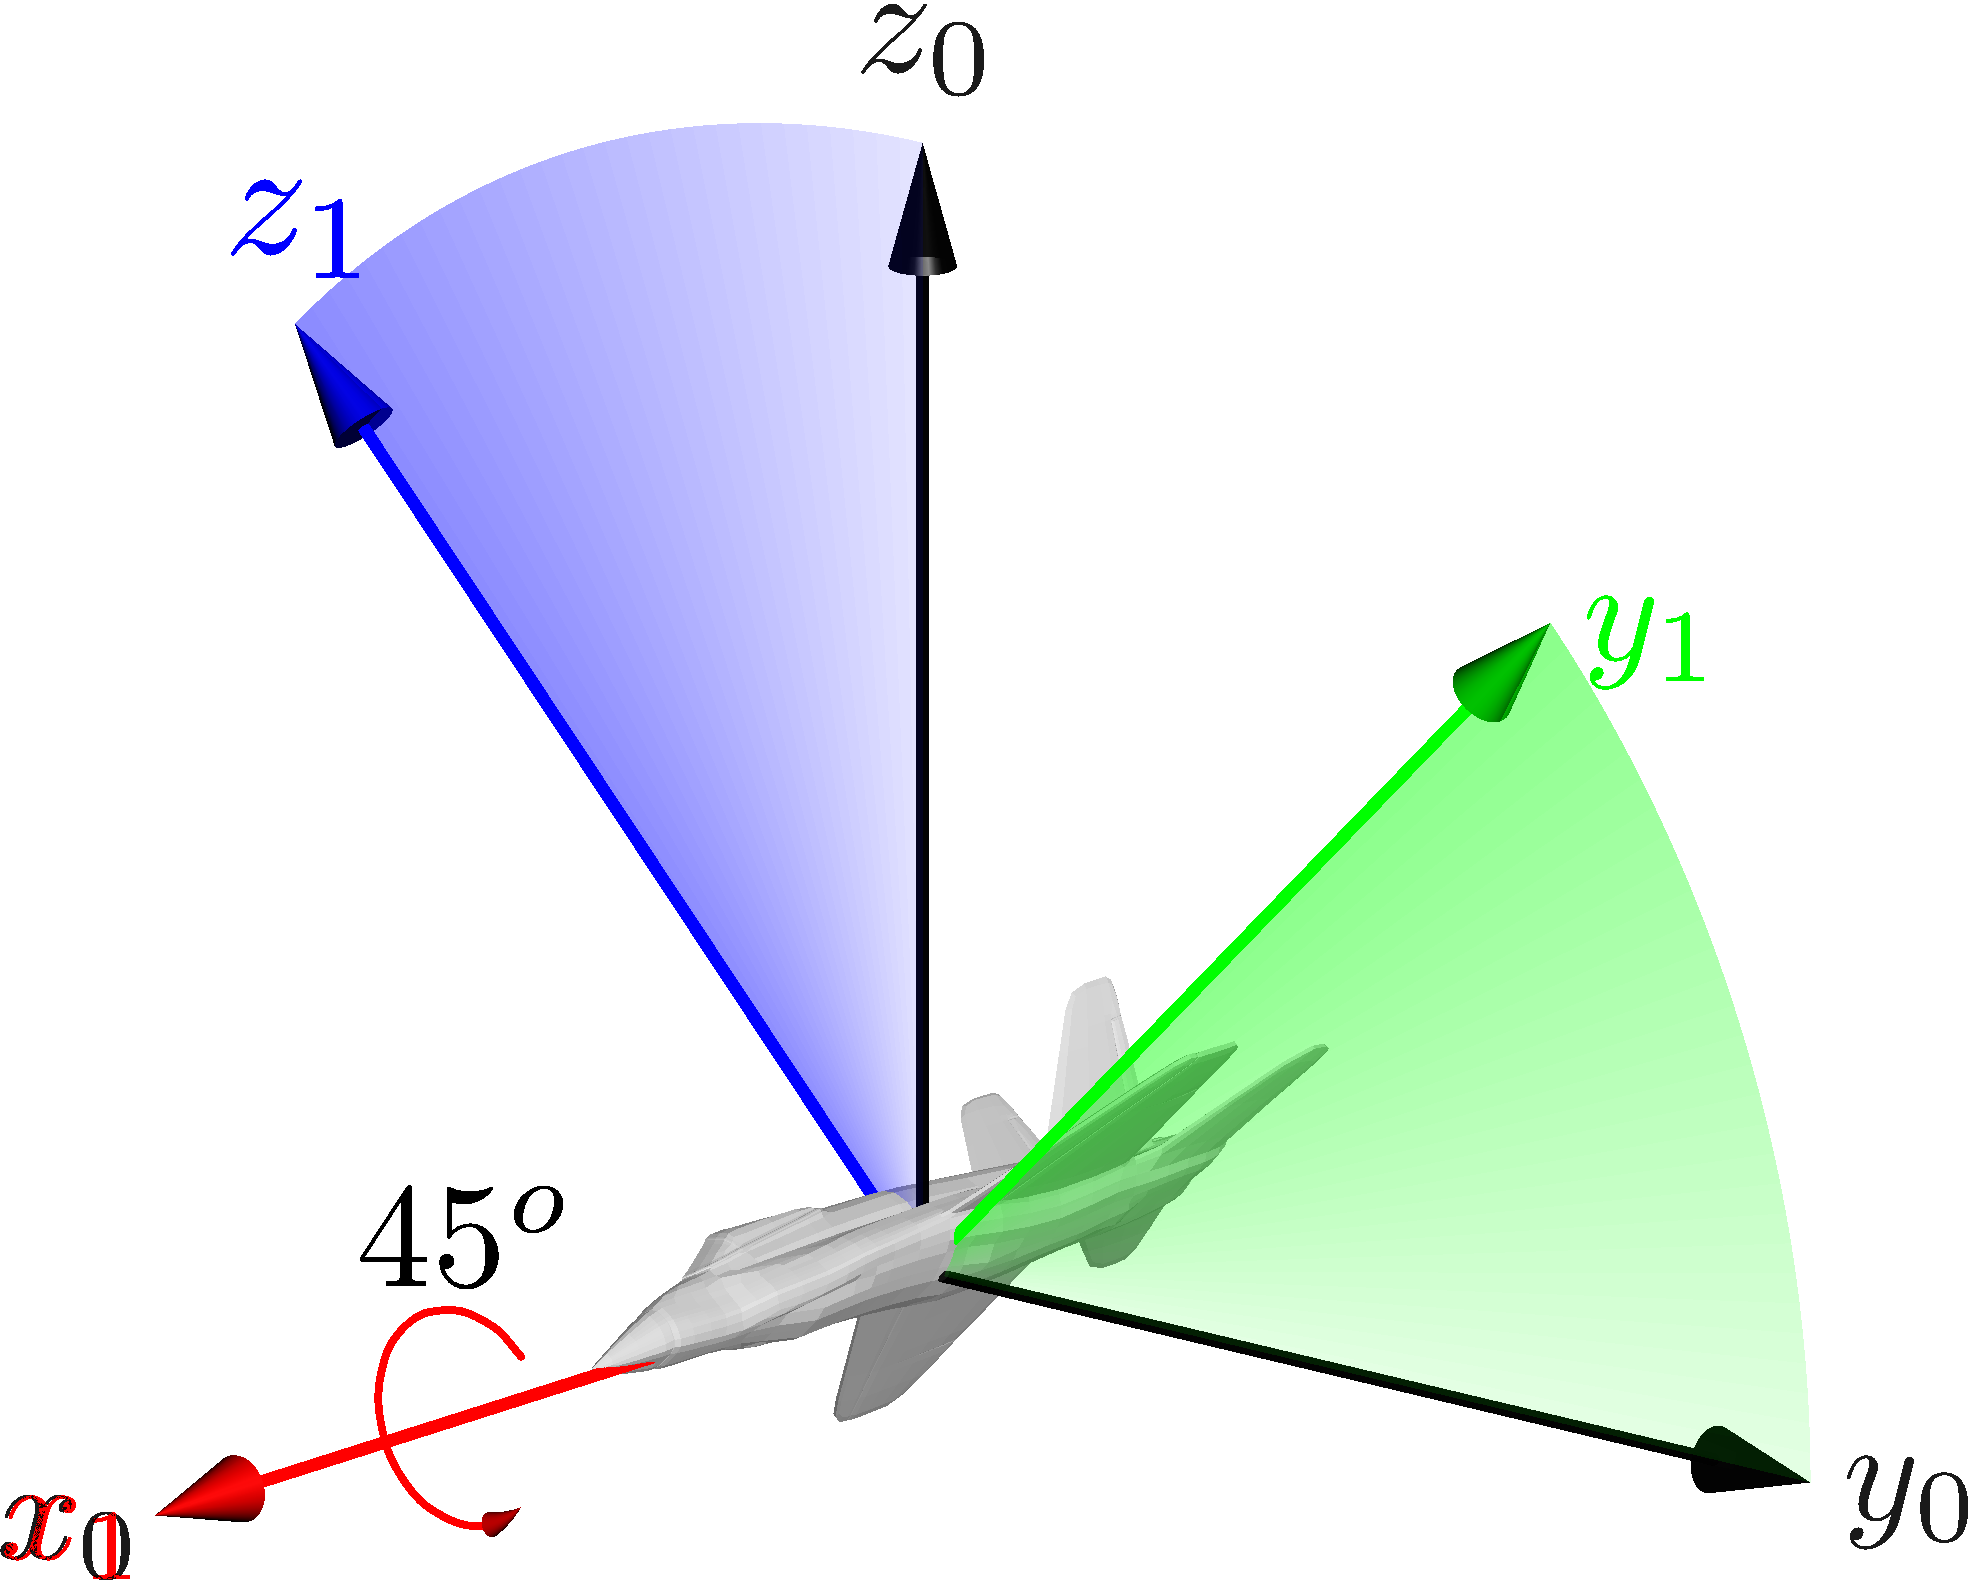
\includegraphics{frames/figs/euler_static_1.png}};
\node[inner sep=0pt] (e2) at (0,0)
    {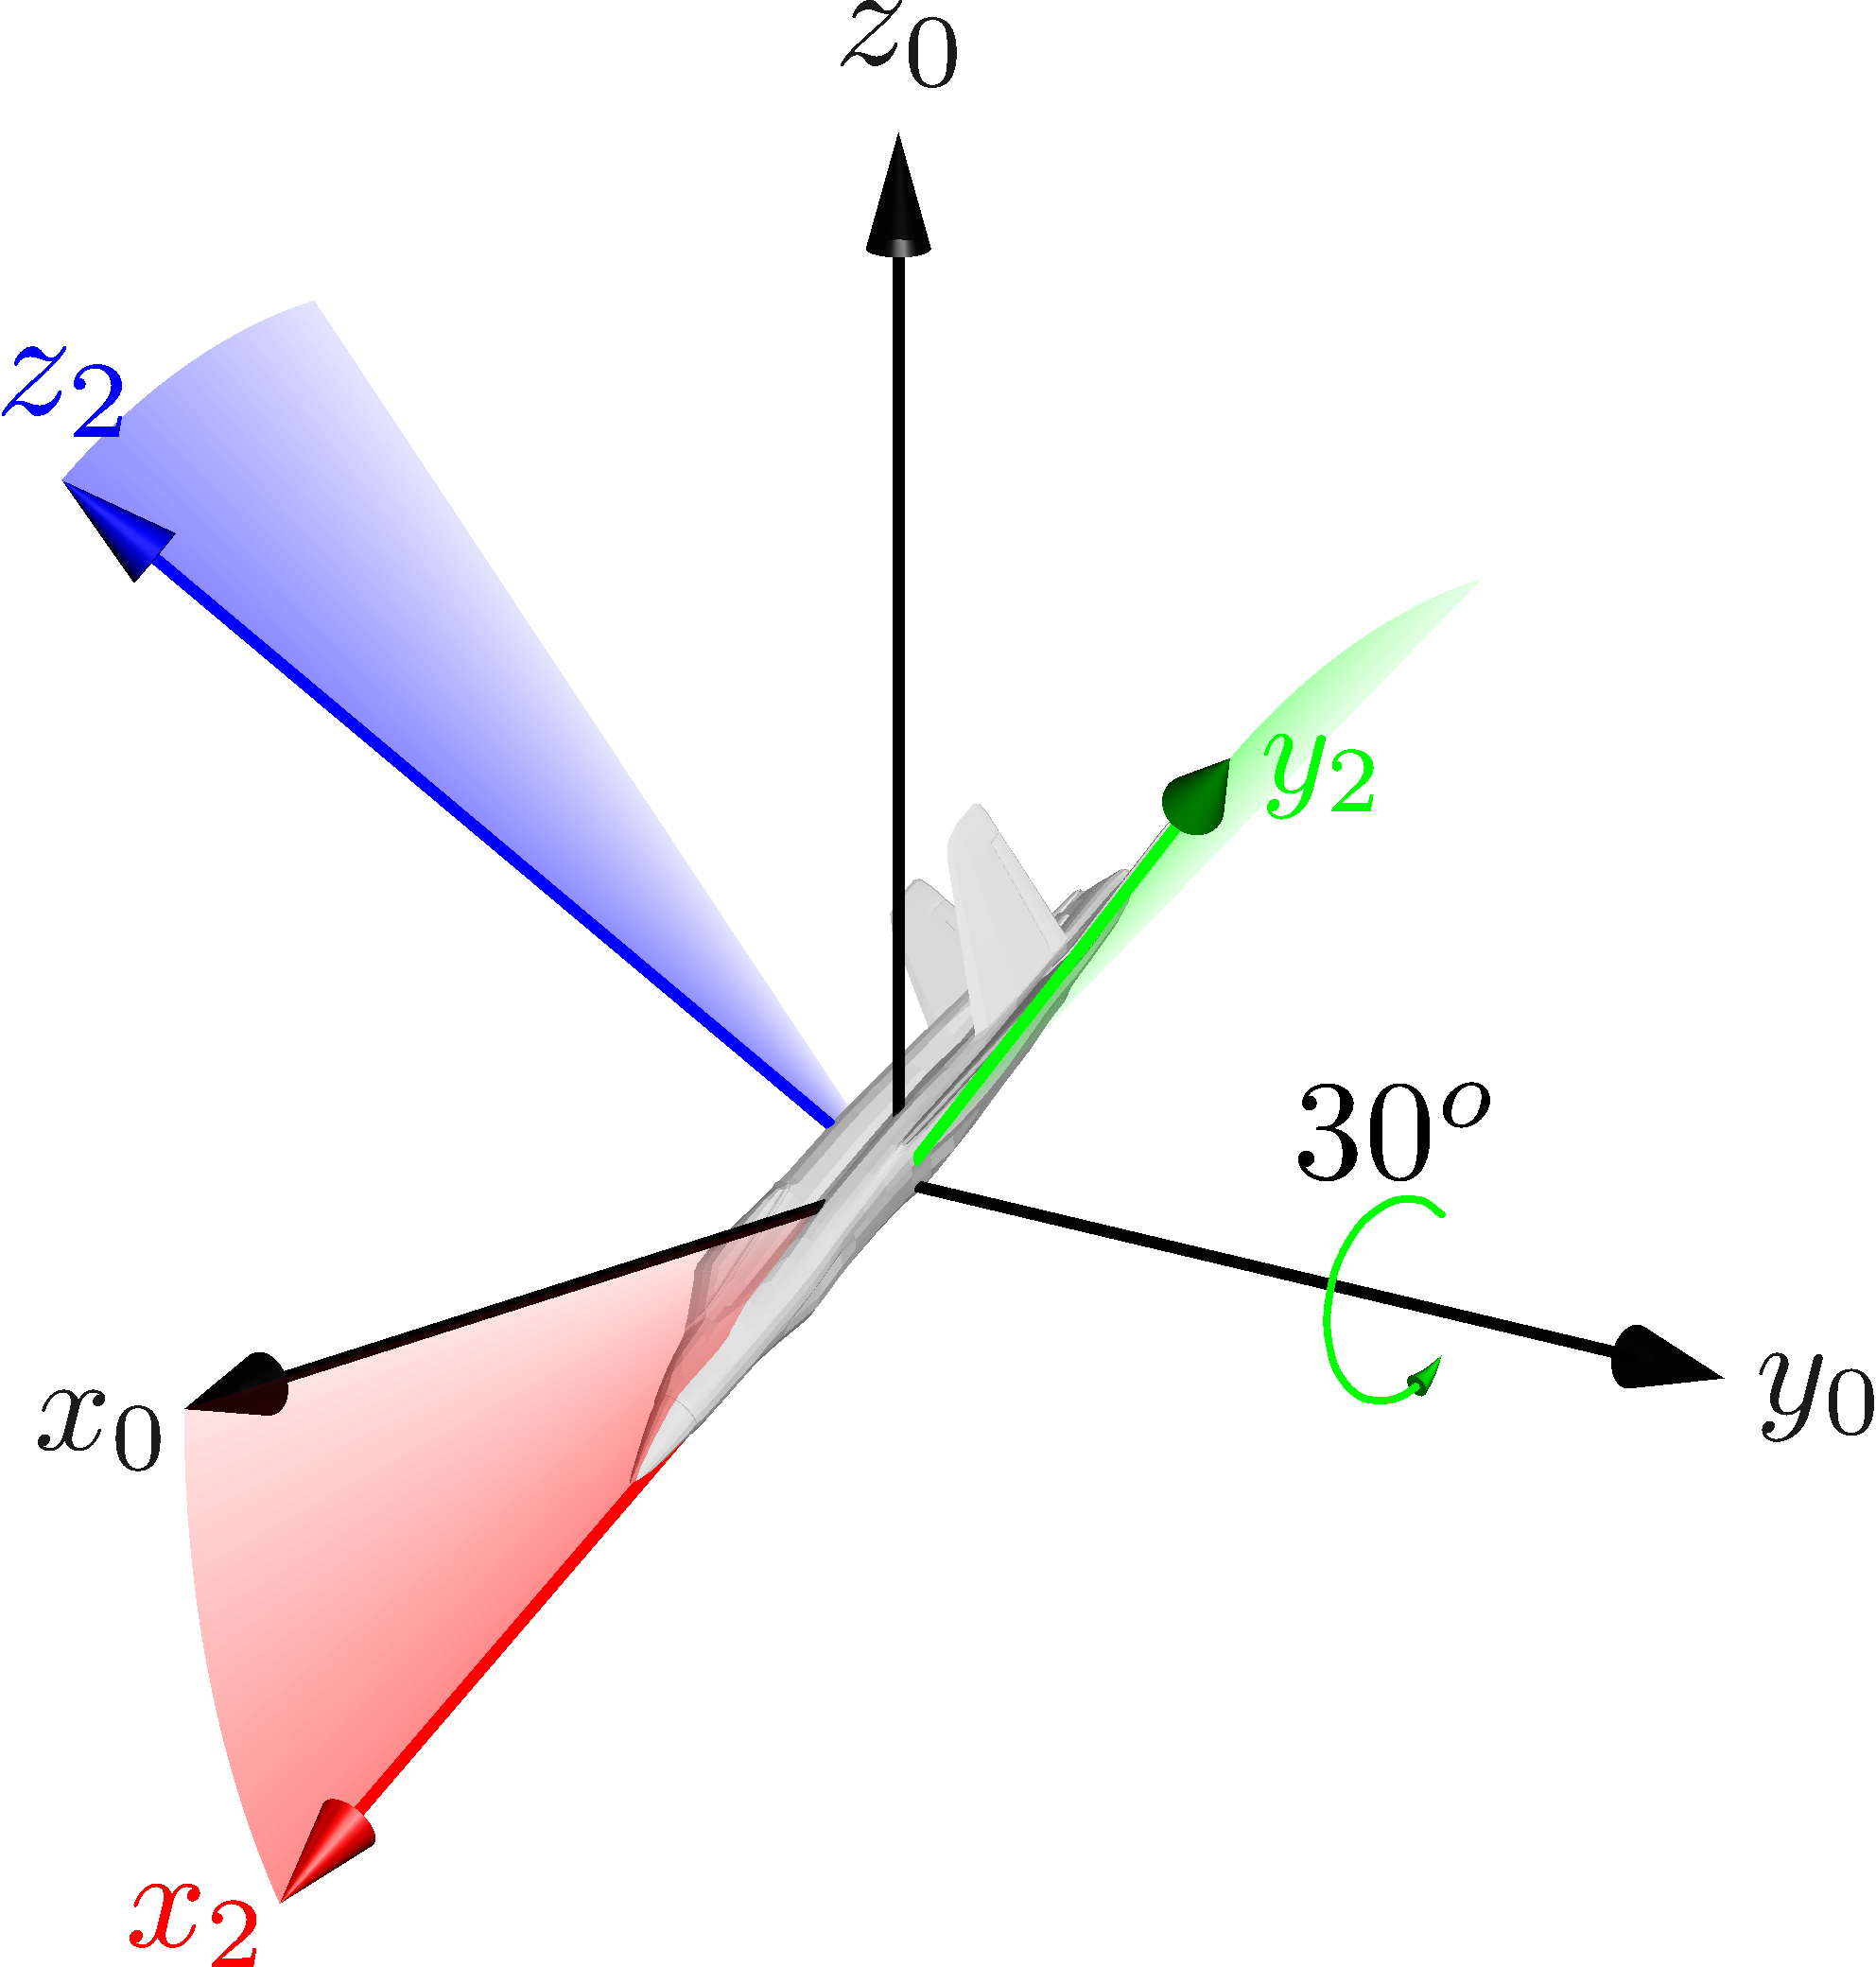
\includegraphics{frames/figs/euler_static_2.png}};
\node[inner sep=0pt] (e3) at (6.0,0)
    {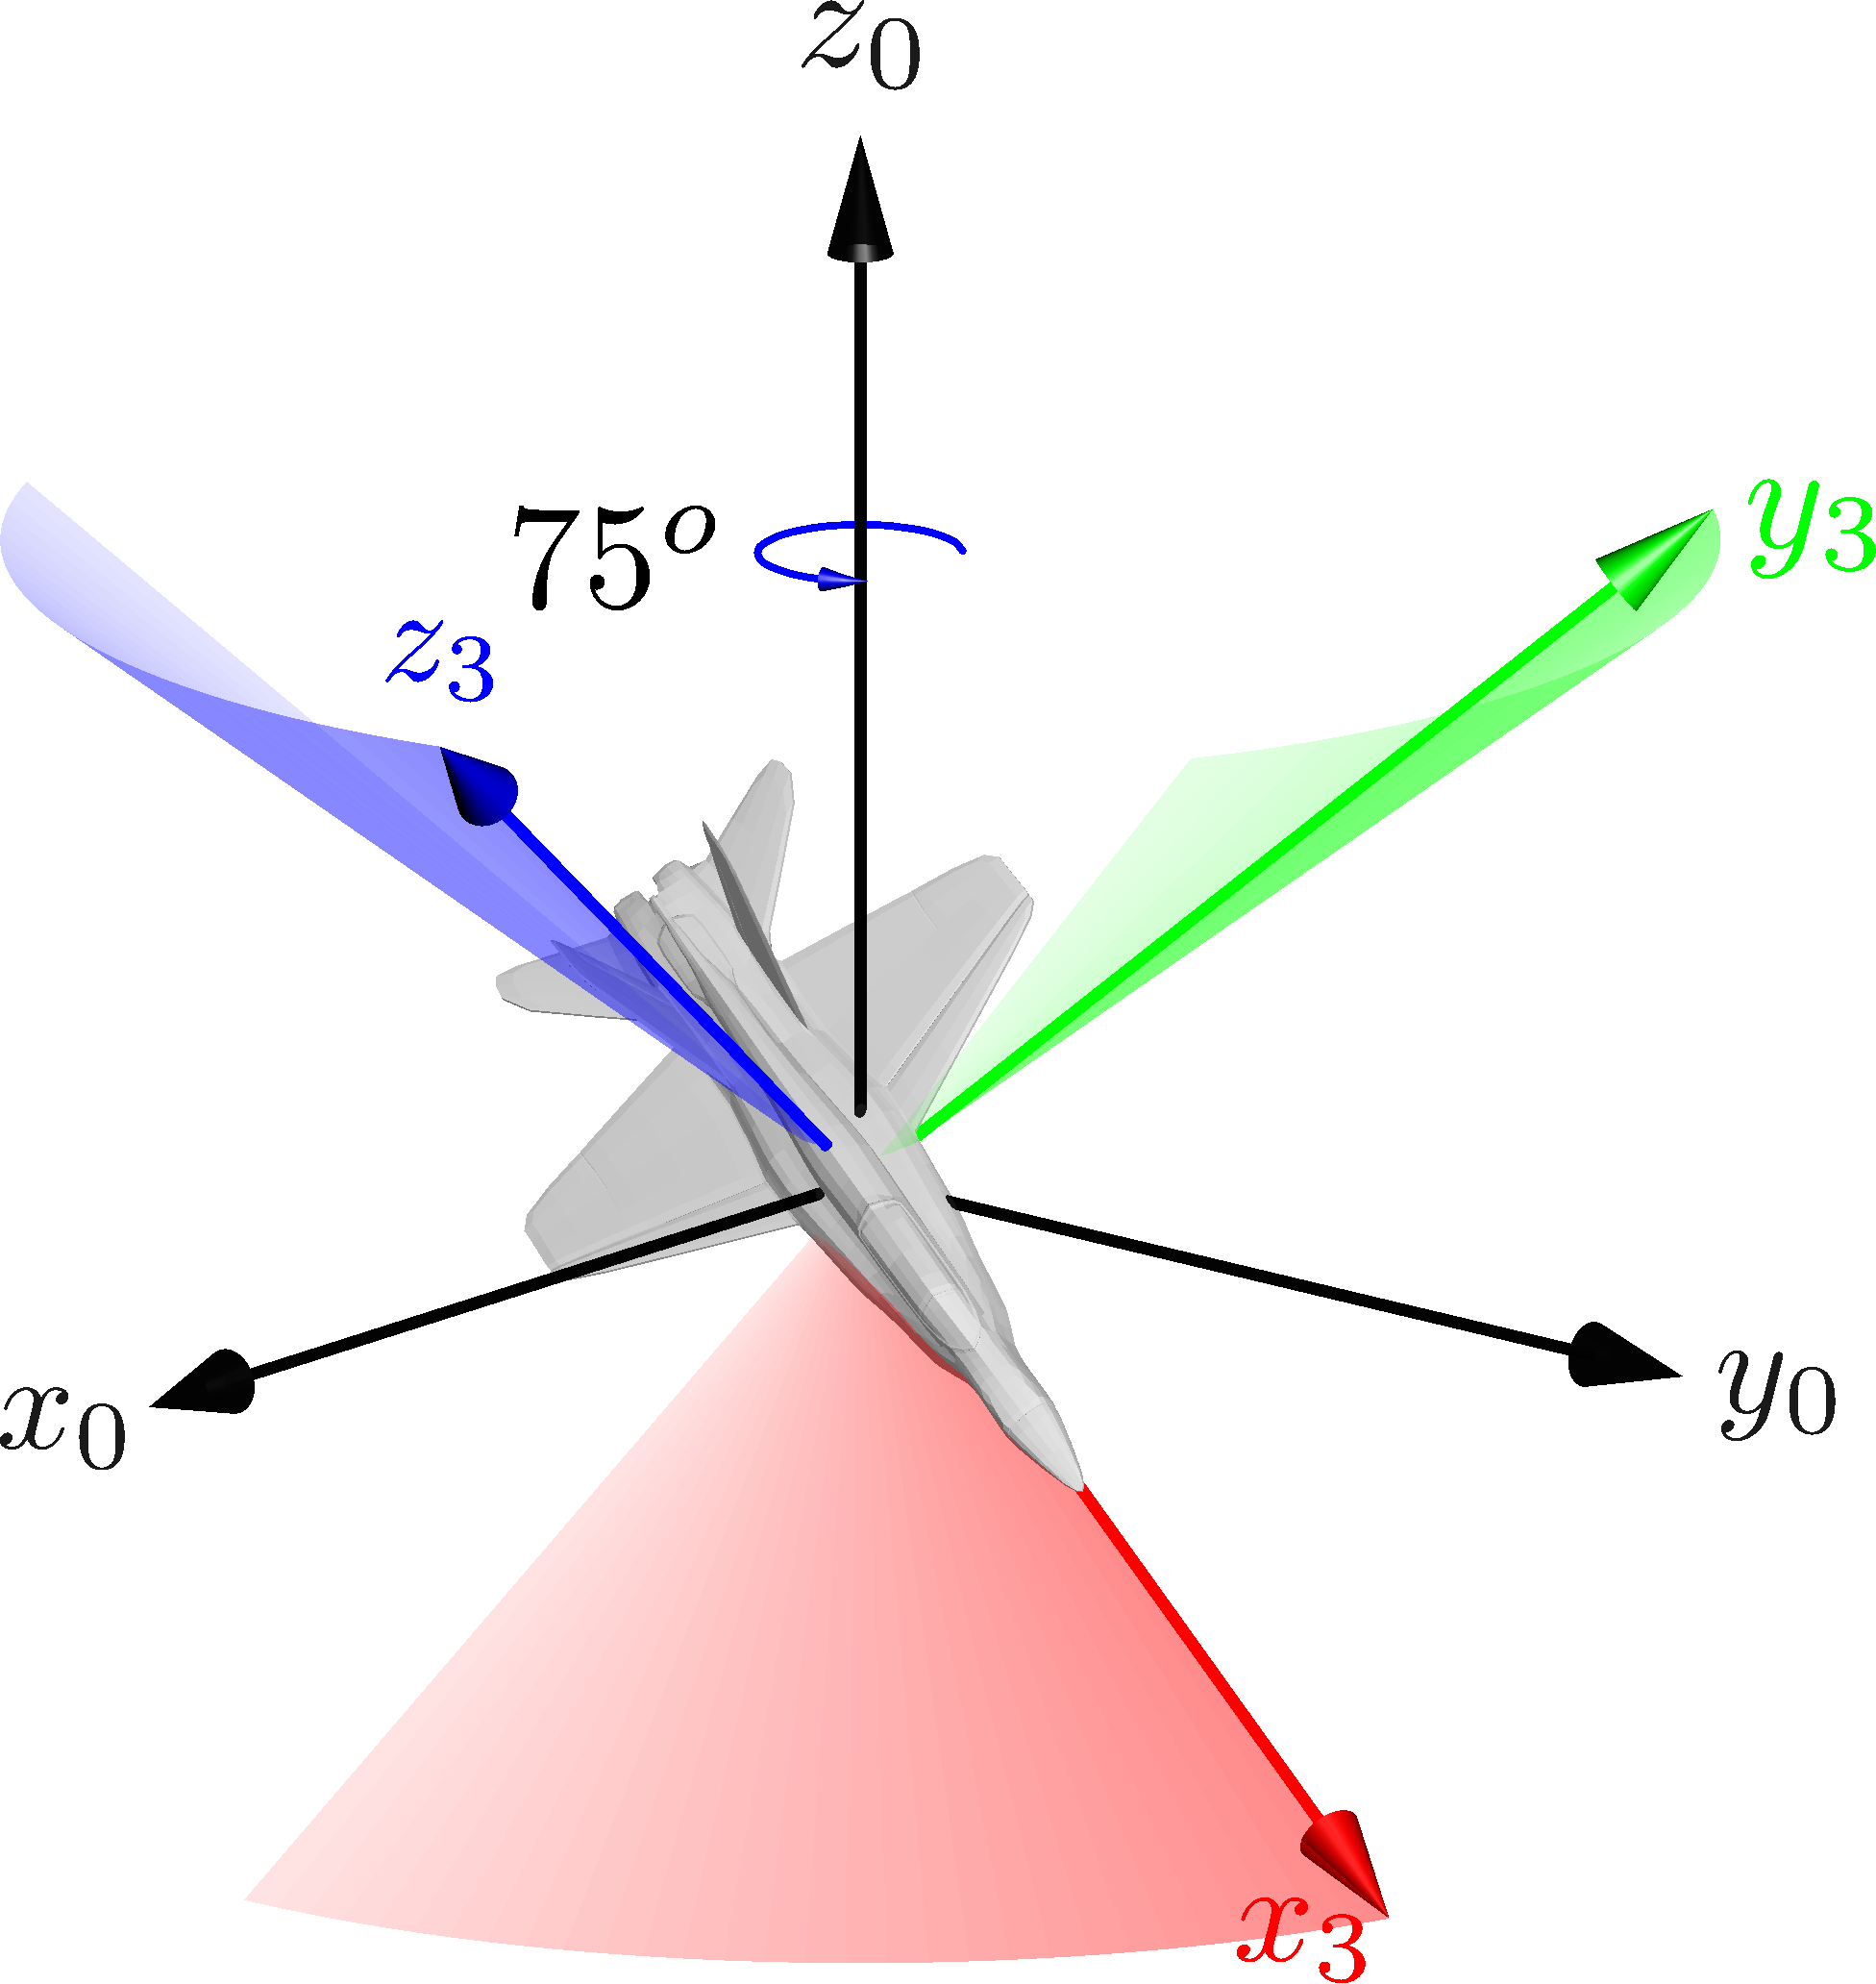
\includegraphics{frames/figs/euler_static_3.png}};
\draw[->,thick,dashed,>=latex,gray] (2,0) -- (3.5,0);
\draw[->,thick,dashed,>=latex,gray] (2,5) -- (3.5,5);
\draw[->,thick,dashed,>=latex,gray] (3.5,3) -- (2,2);
\end{tikzpicture}

\end{center}
\caption{Static}
\label{fig:static_rotations}
\end{figure}


\begin{figure}
\begin{center}

\begin{tikzpicture}

\node[inner sep=0pt] (e0) at (0,5.0)
    {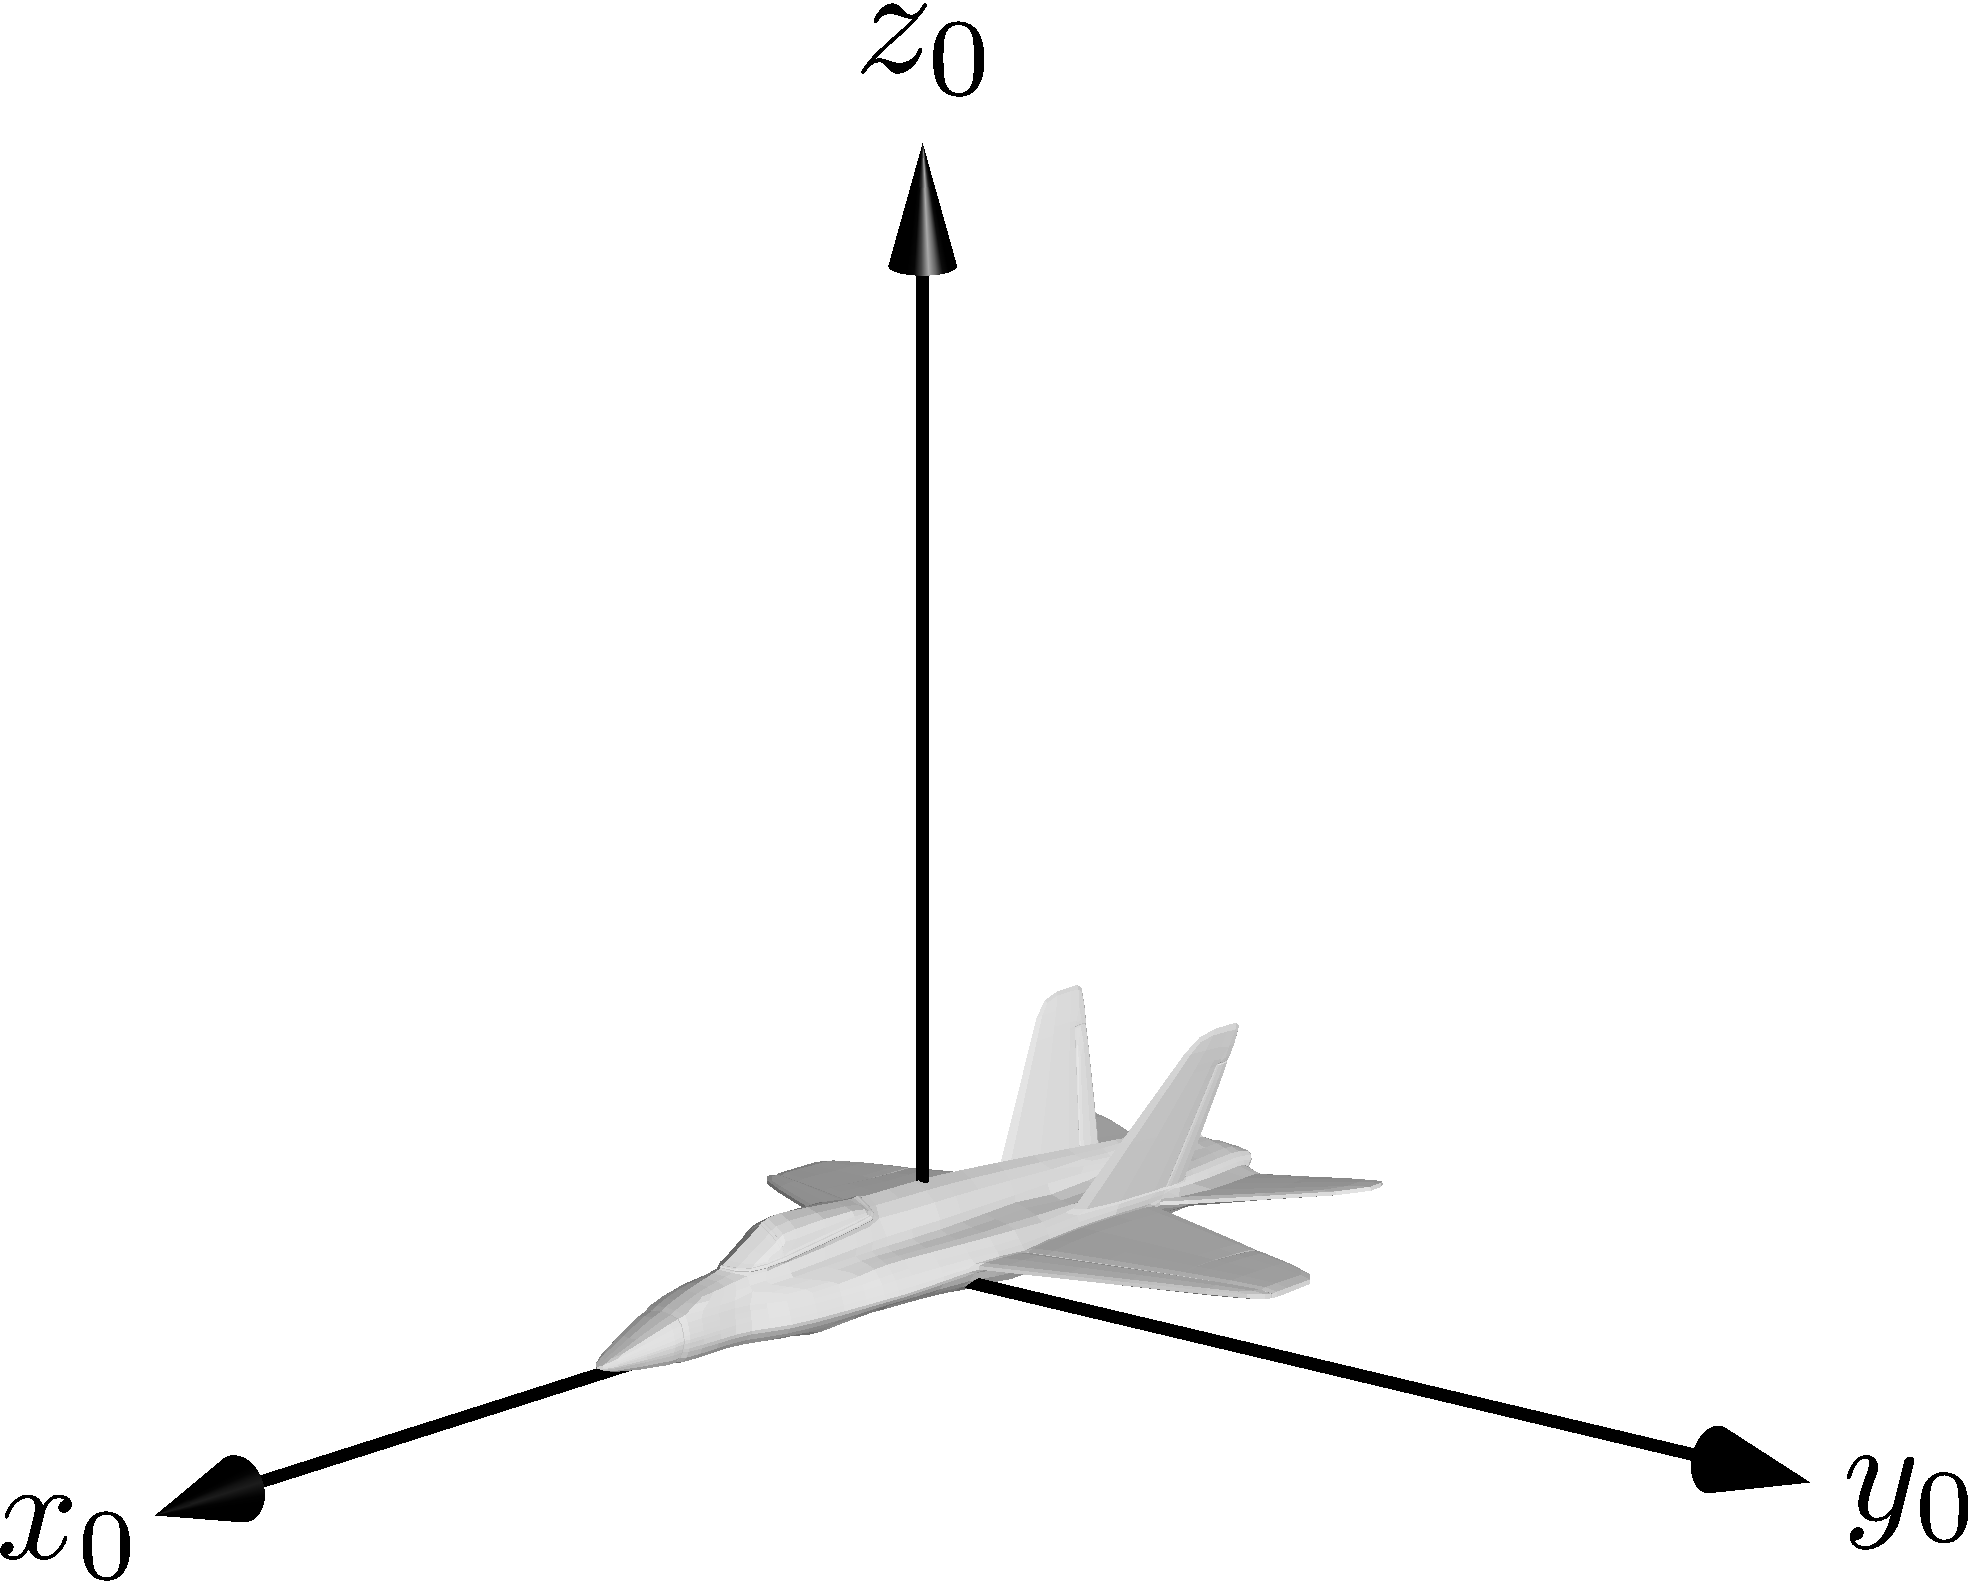
\includegraphics{frames/figs/euler_nonstatic_0.png}};
\node[inner sep=0pt] (e1) at (6.0,5.0)
    {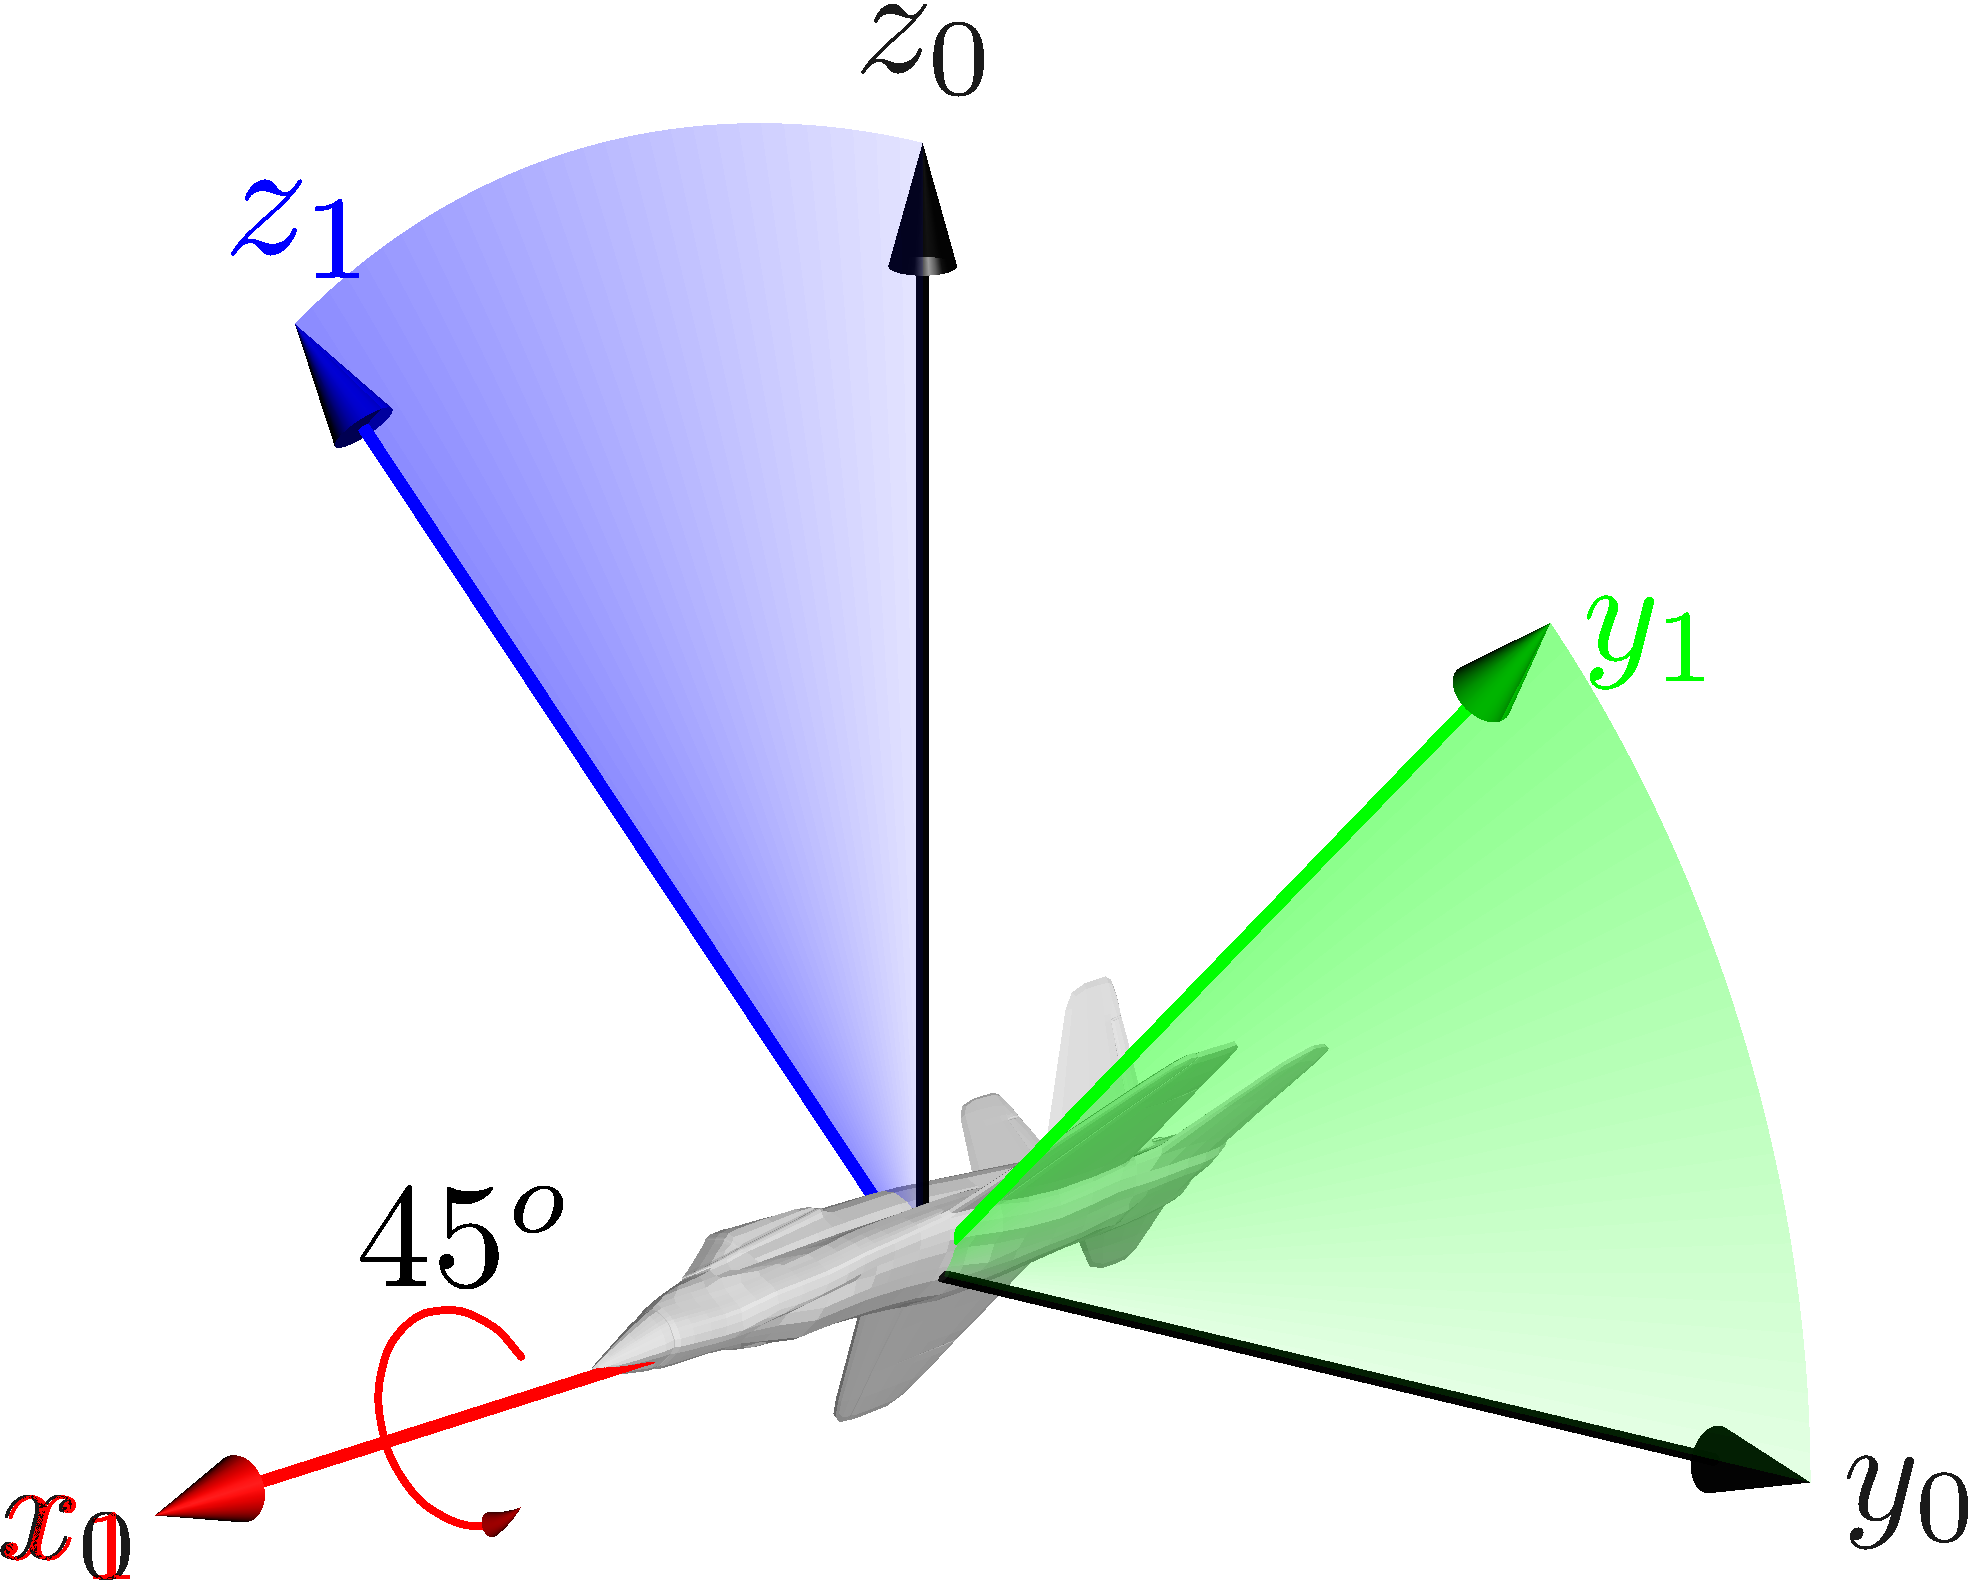
\includegraphics{frames/figs/euler_nonstatic_1.png}};
\node[inner sep=0pt] (e2) at (0,0)
    {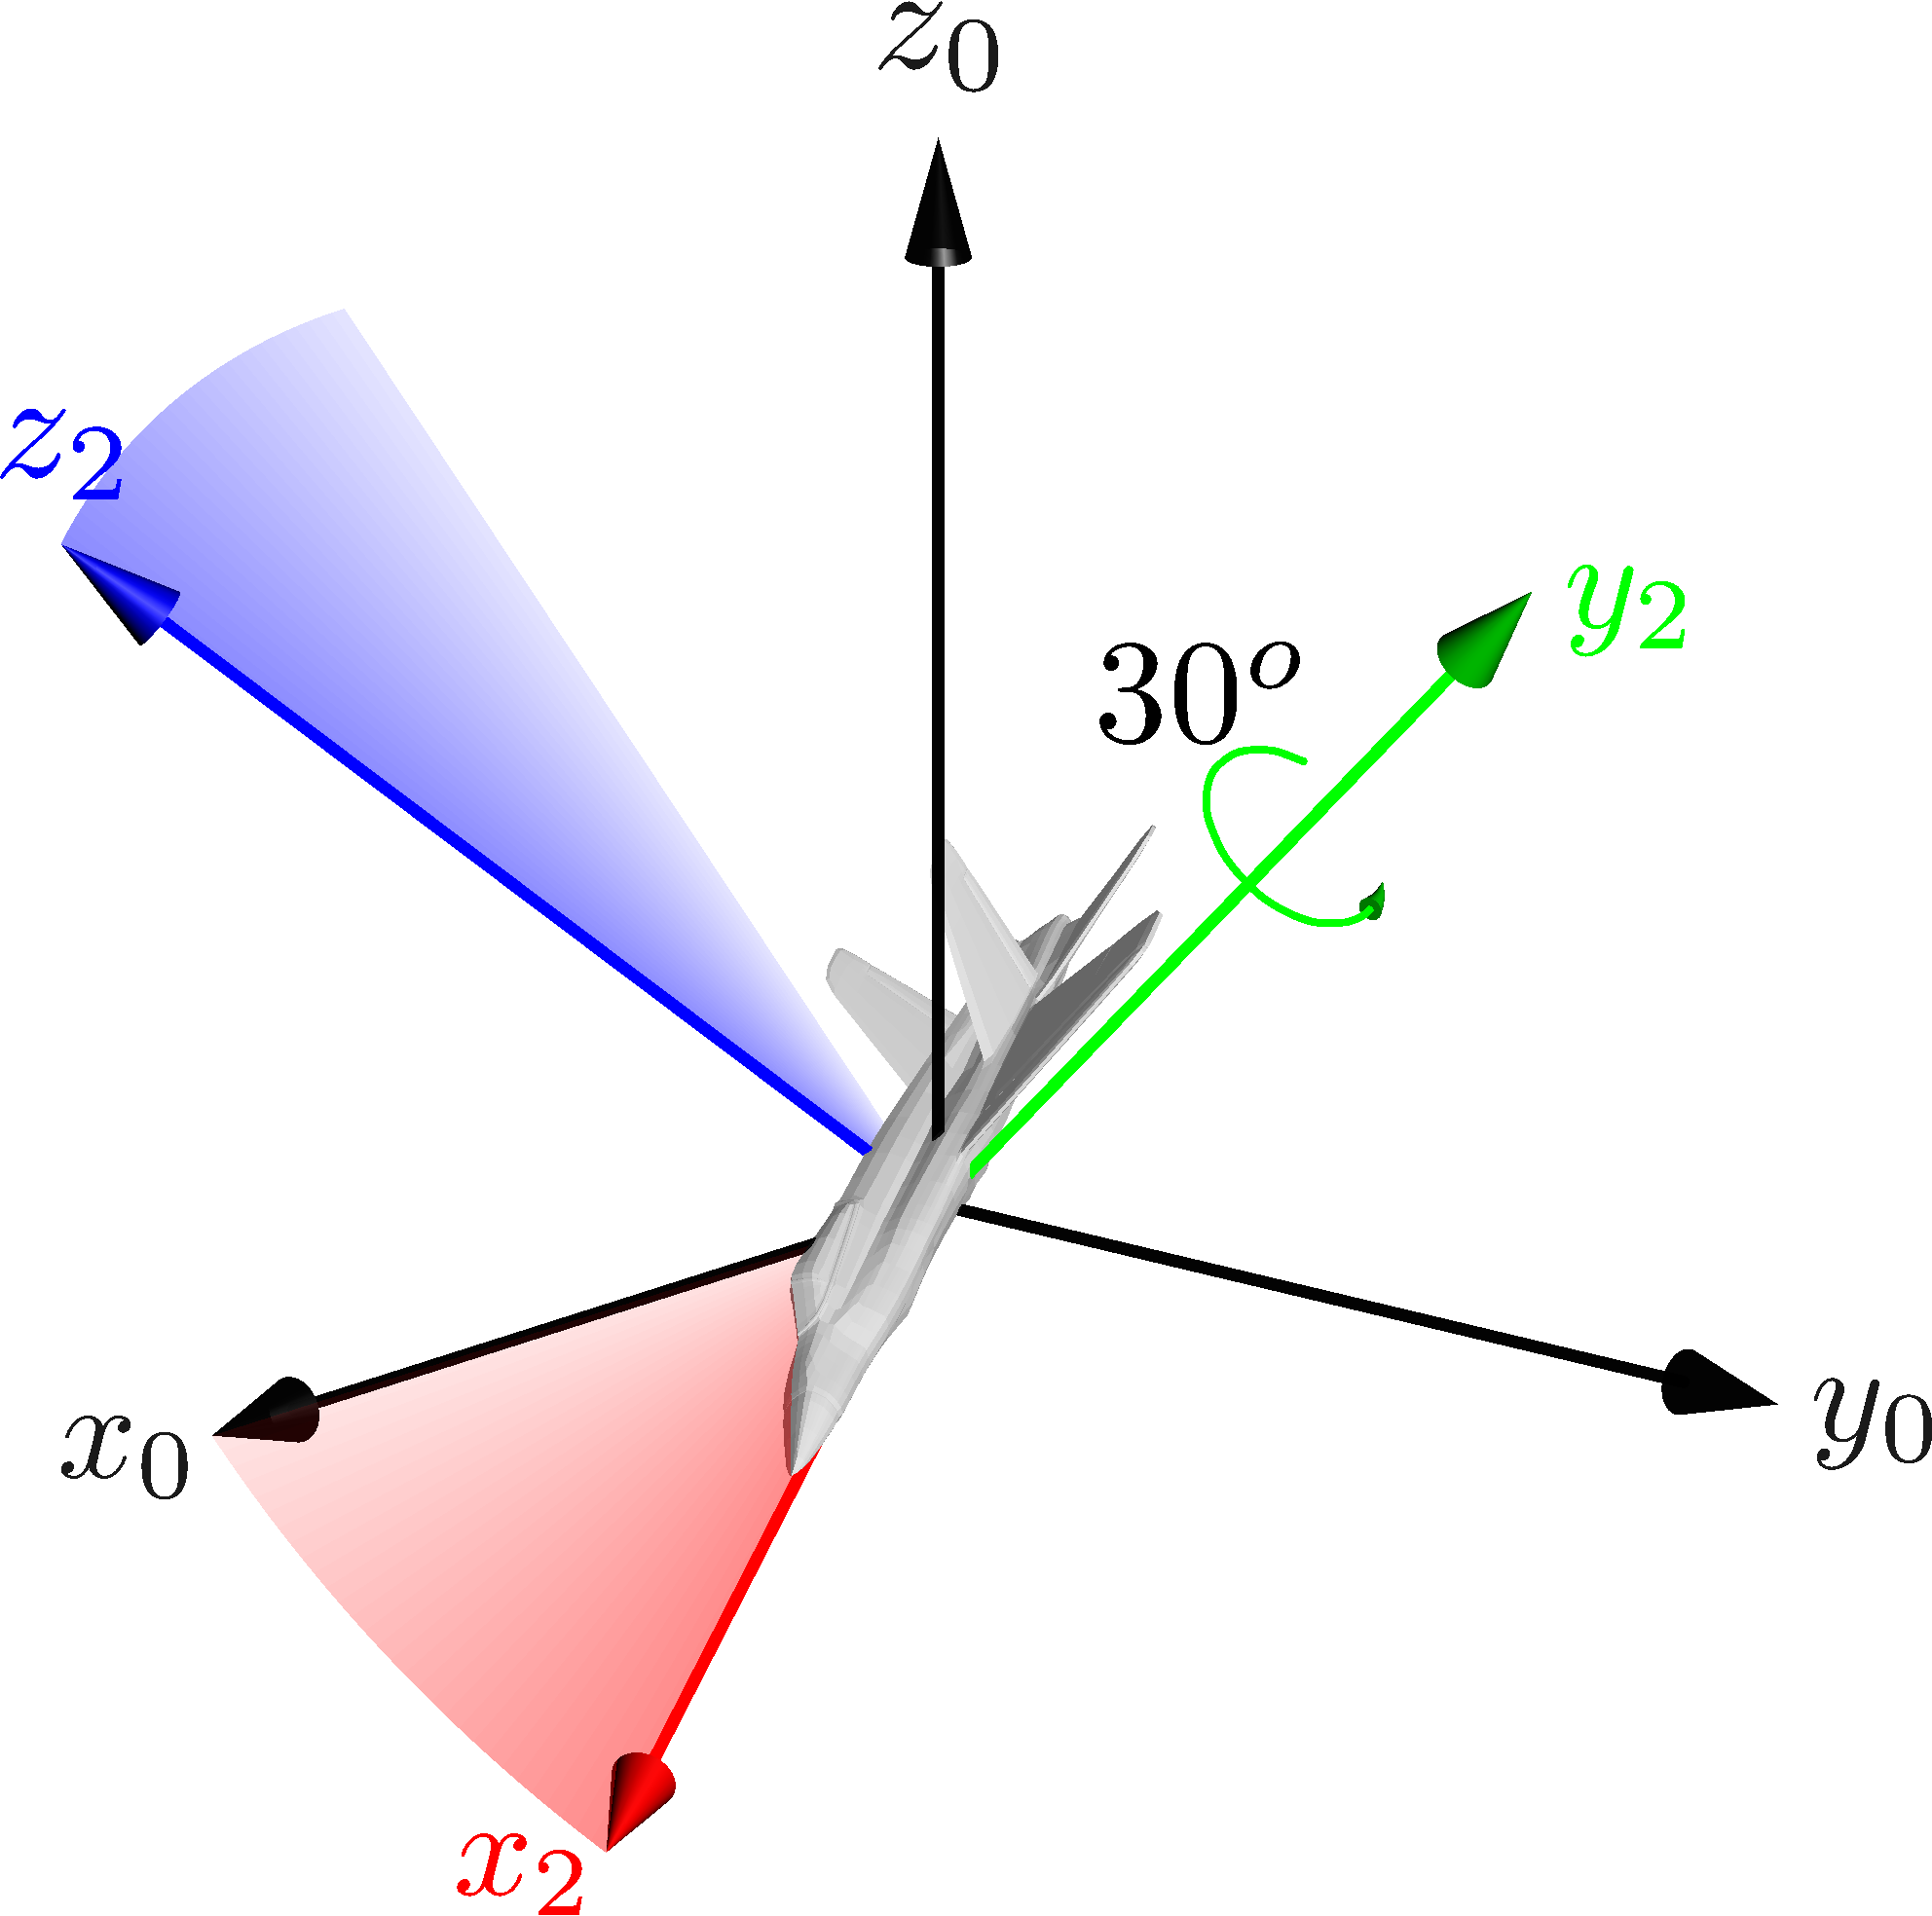
\includegraphics{frames/figs/euler_nonstatic_2.png}};
\node[inner sep=0pt] (e3) at (6.0,0)
    {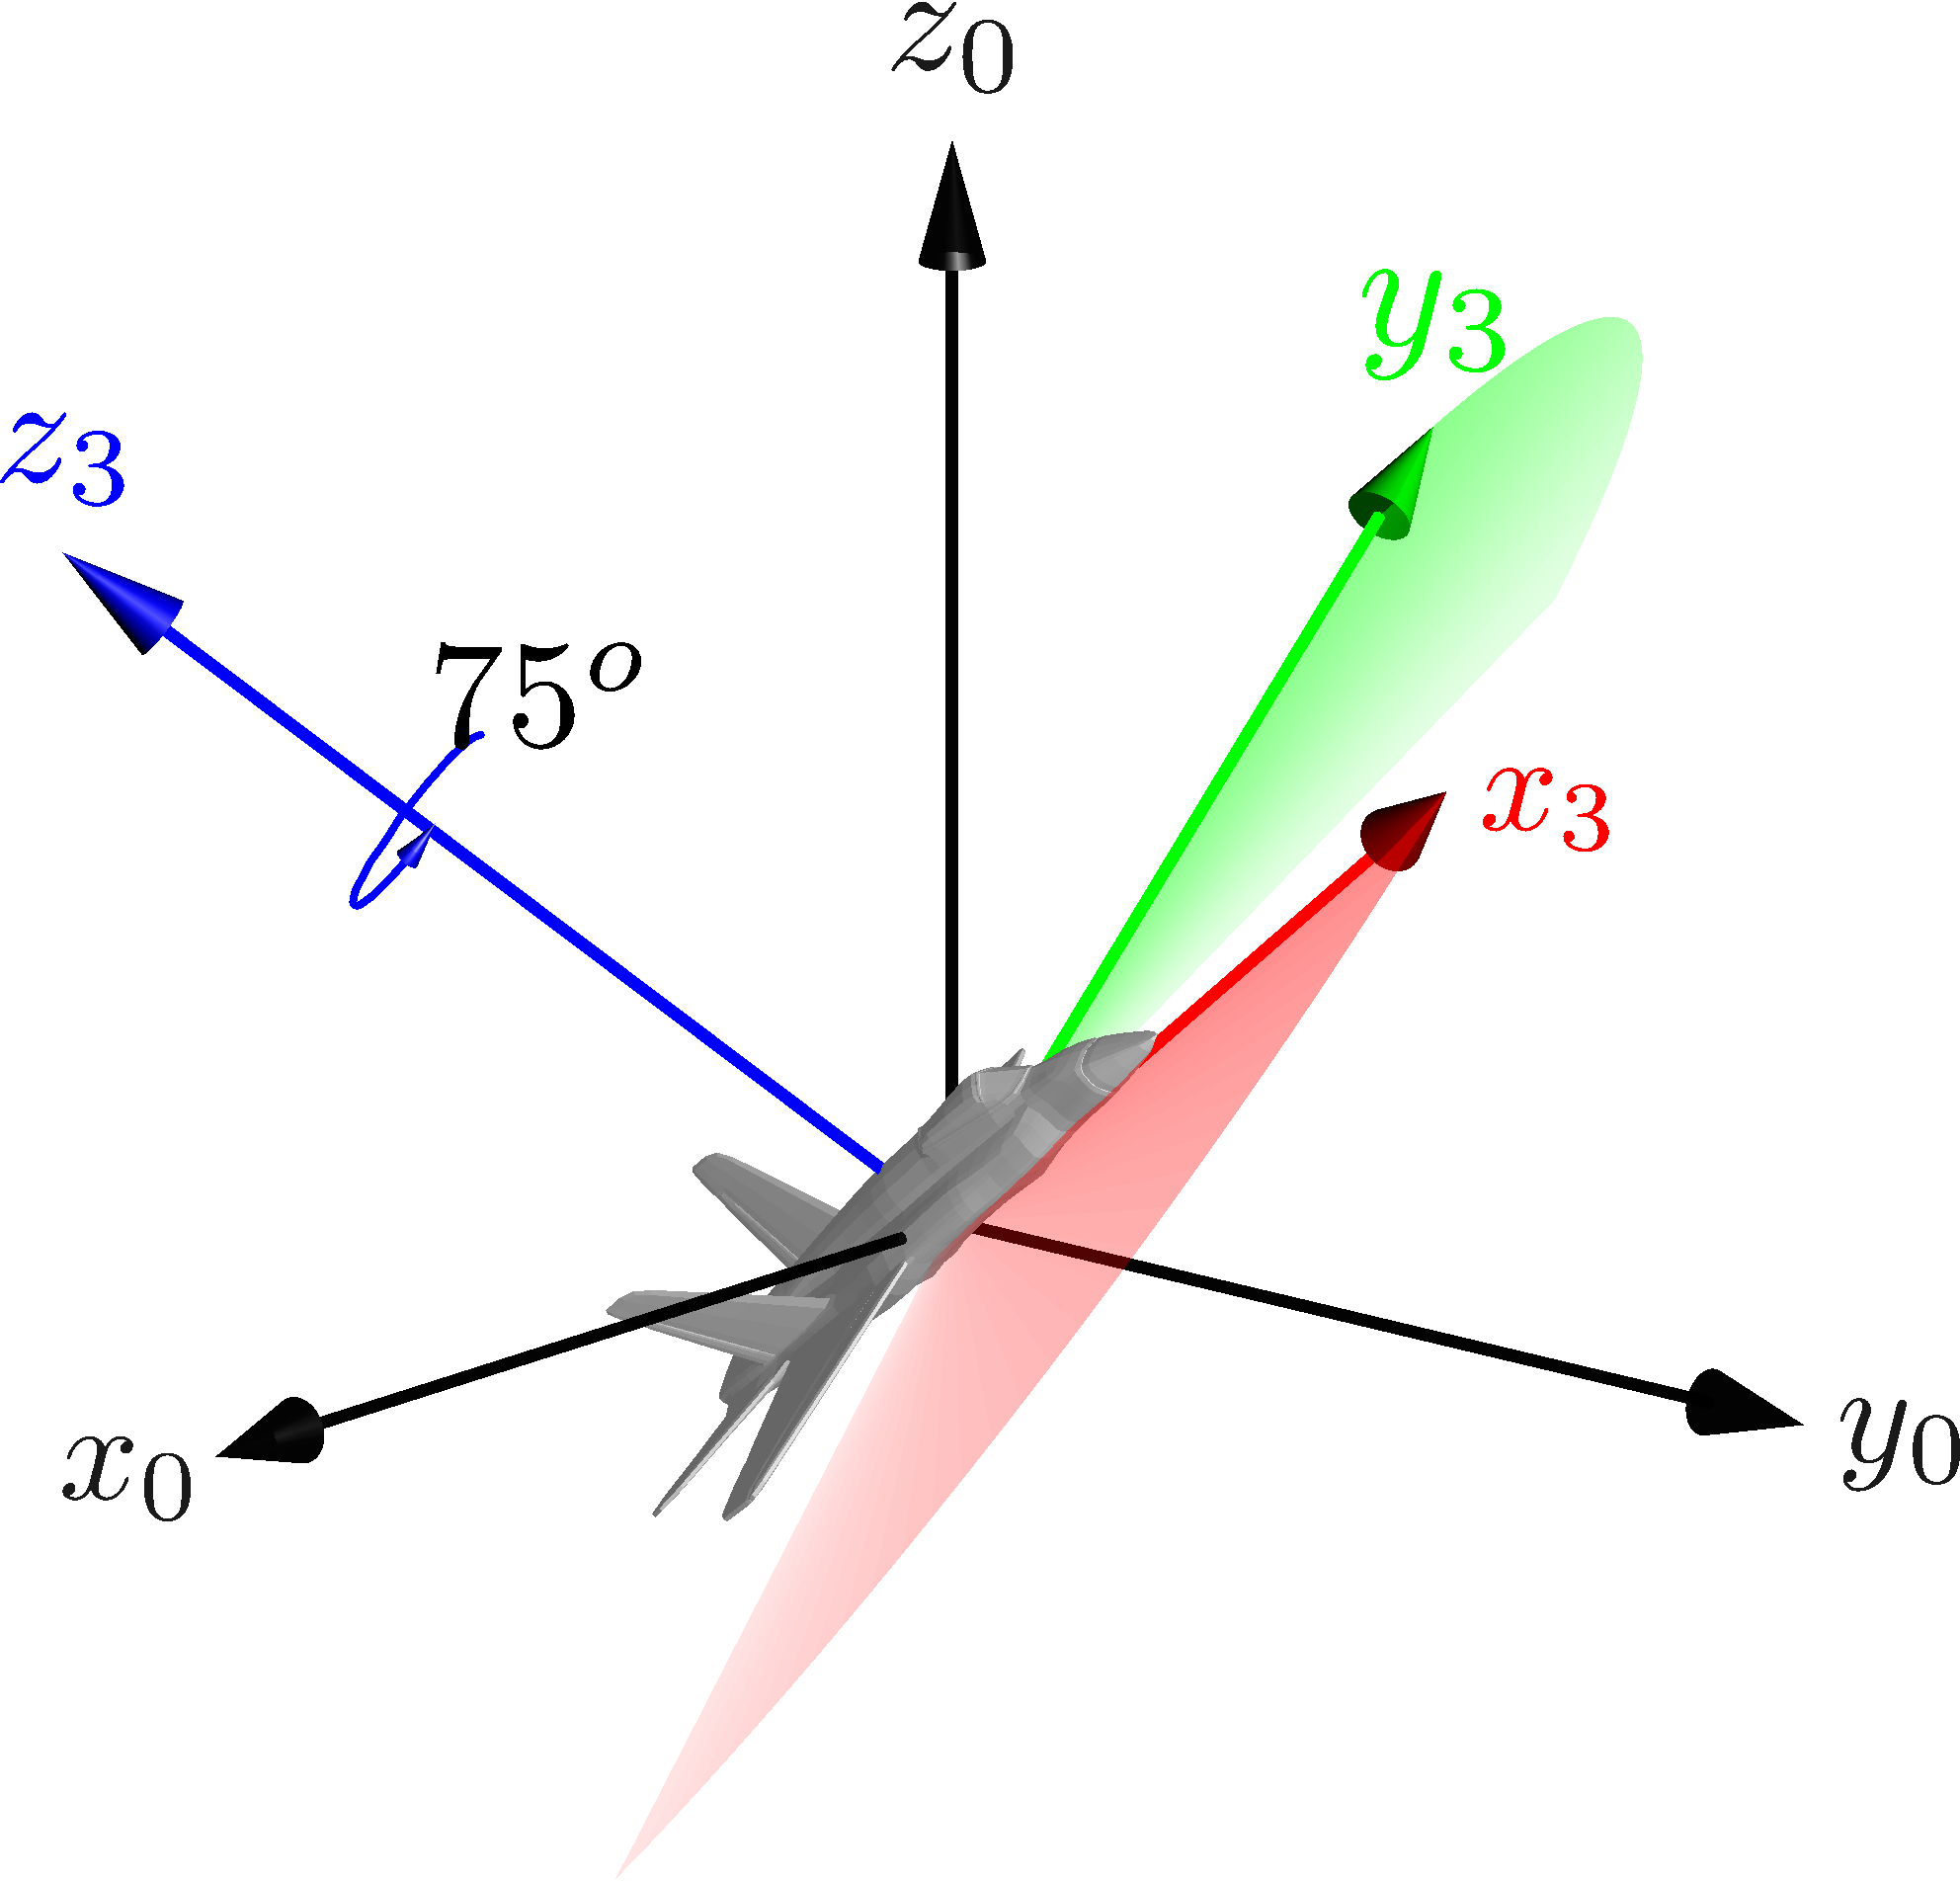
\includegraphics{frames/figs/euler_nonstatic_3.png}};


\draw[->,thick,dashed,>=latex,gray] (2,0) -- (3.5,0);
\draw[->,thick,dashed,>=latex,gray] (2,5) -- (3.5,5);
\draw[->,thick,dashed,>=latex,gray] (3.5,3) -- (2,2);

%\draw[->,thick,dashed,>=latex] (e1.south west) -- (e2.north east);
%\draw[->,thick,dashed,>=latex] (e2.east) -- (e3.west);
\end{tikzpicture}

\end{center}
\caption{Non static}
\label{fig:nonstatic_rotations}
\end{figure}




It is also necessary to specify whether the rotations are relative to
the parent coordinate frame, or whether each rotation is performed
around the axes of a coordinate frame aligned with the earlier
rotations.  These two alternatives are illustrated in Figures
\ref{fig:static_rotations} and \ref{fig:nonstatic_rotations}.  The
first alternative is sometimes referred to as ``static'' or
``extrinsic'' rotations, while the second may be referred to as
``relative'' or ``intrinsic'' rotations.  Combined with the choice of
axis orderings, this means that there are twenty-four possible
conventions for specifying Euler angles.

Euler angles are relatively easy to visualize, but they are
inconvenient to work with from a mathematical point of view.  The key
problem is that the mapping from spatial orientations to Euler angles
is discontinuous: small changes in orientation may cause big jumps in
the required representation.  This can cause difficulties when we need
to smoothly update the orientation of a moving object over time.

\subsection{Axis Angle}

\begin{figure}
\begin{center}

\begin{tikzpicture}

\node[inner sep=0pt] (e2) at (0,0)
    {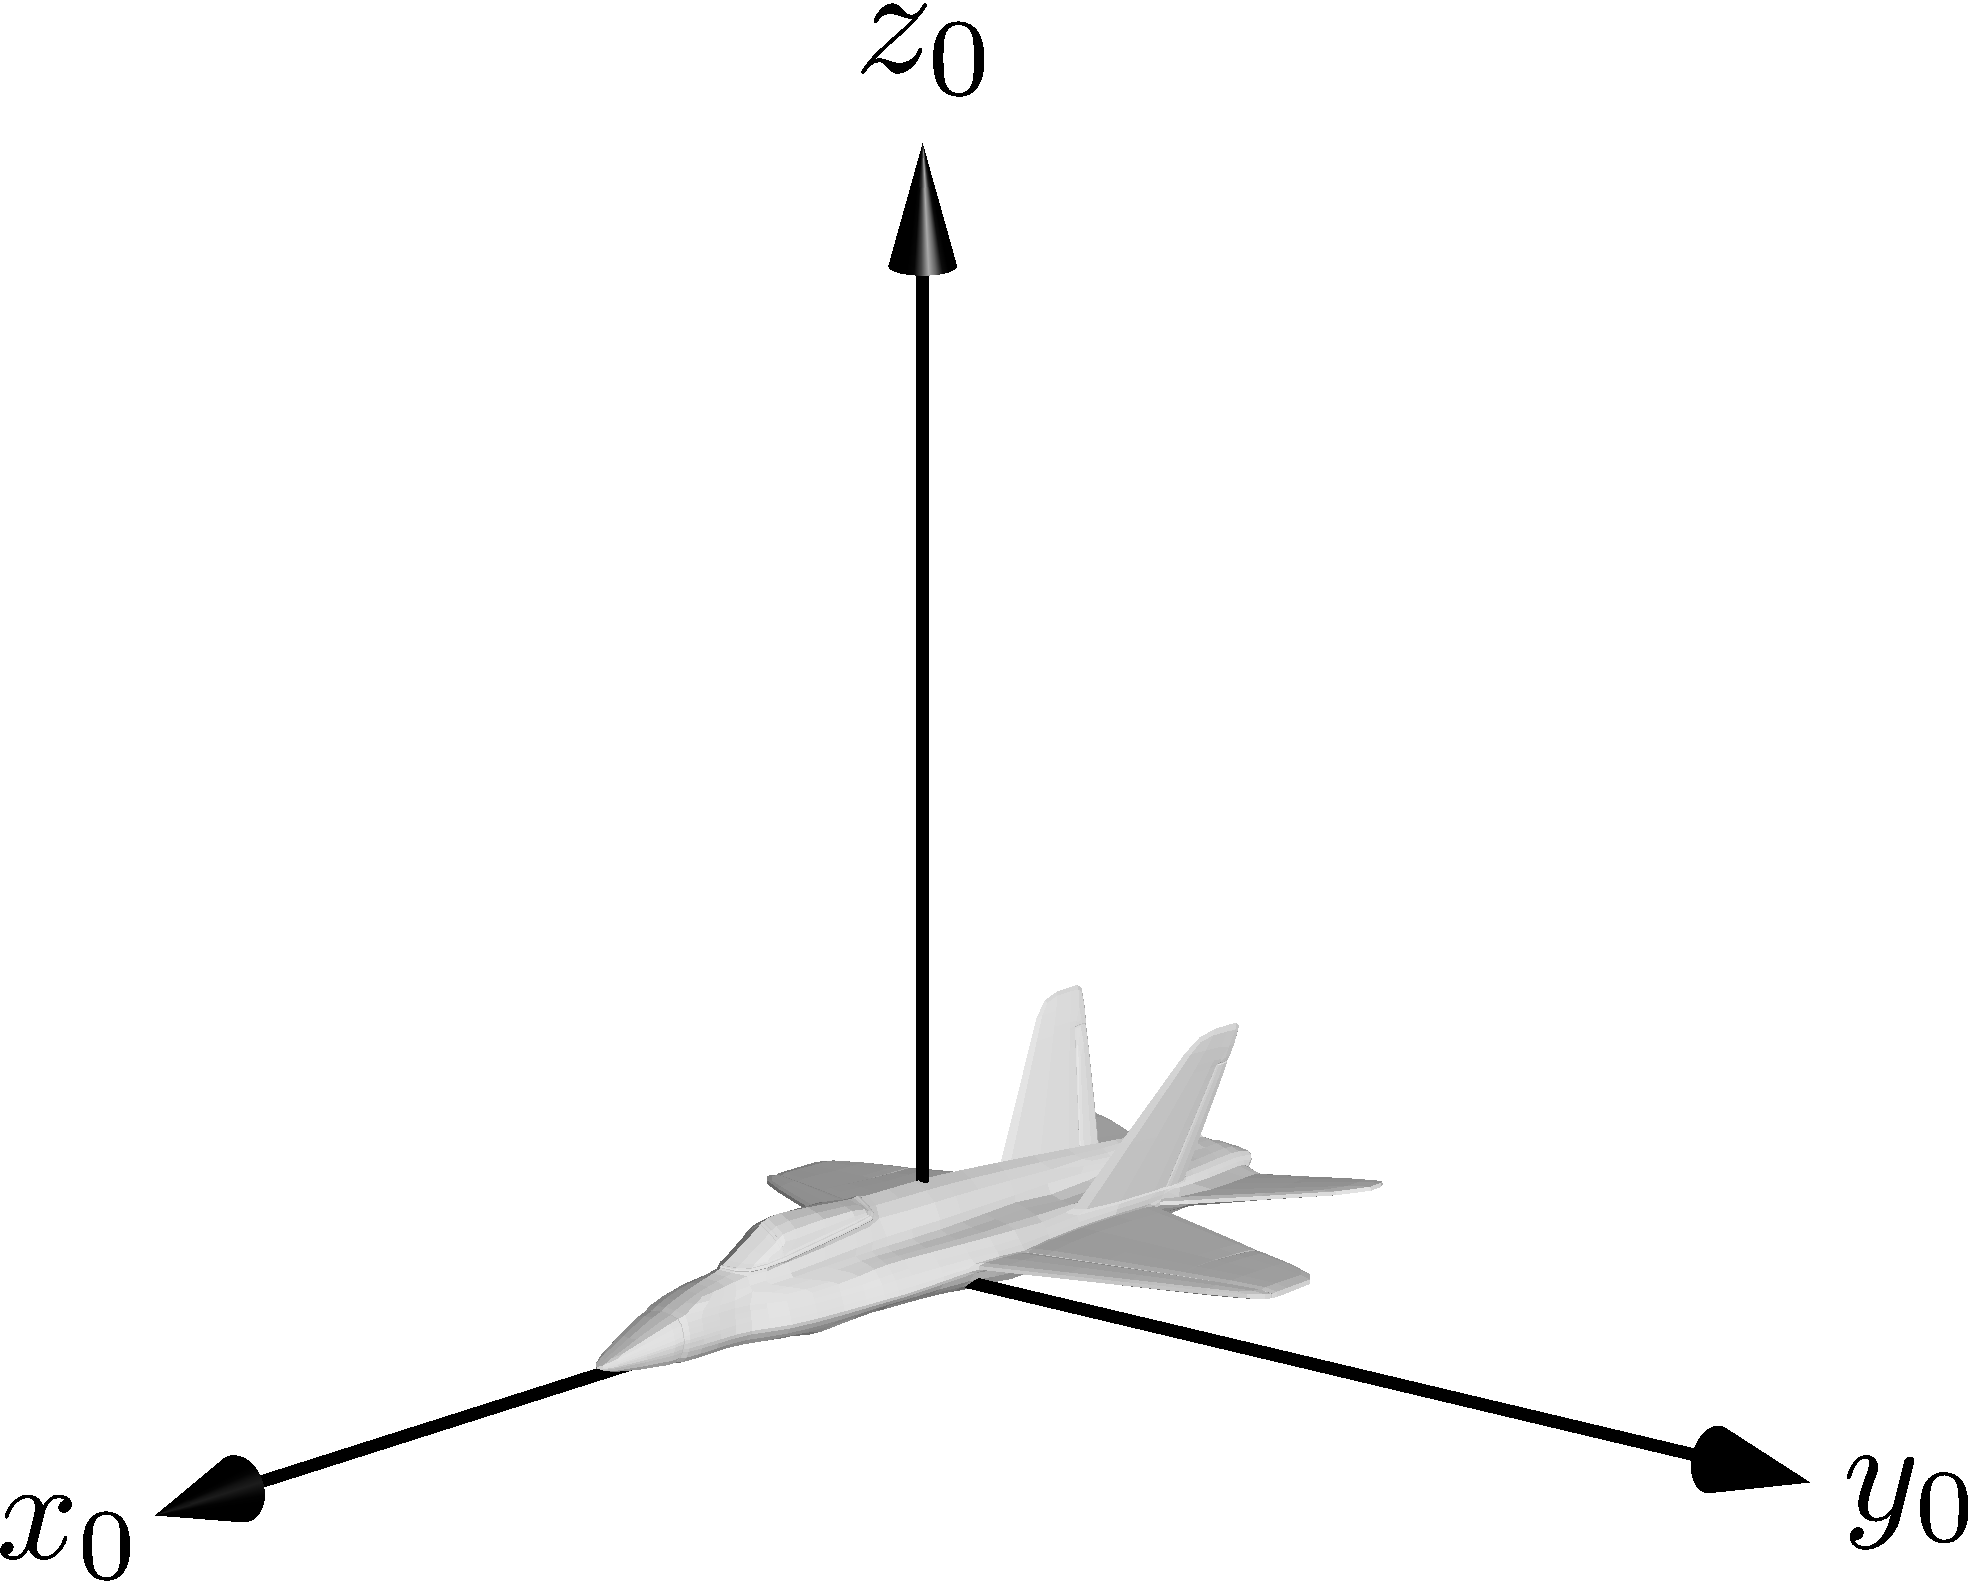
\includegraphics{frames/figs/euler_nonstatic_0.png}};
\node[inner sep=0pt] (e3) at (6.0,0)
    {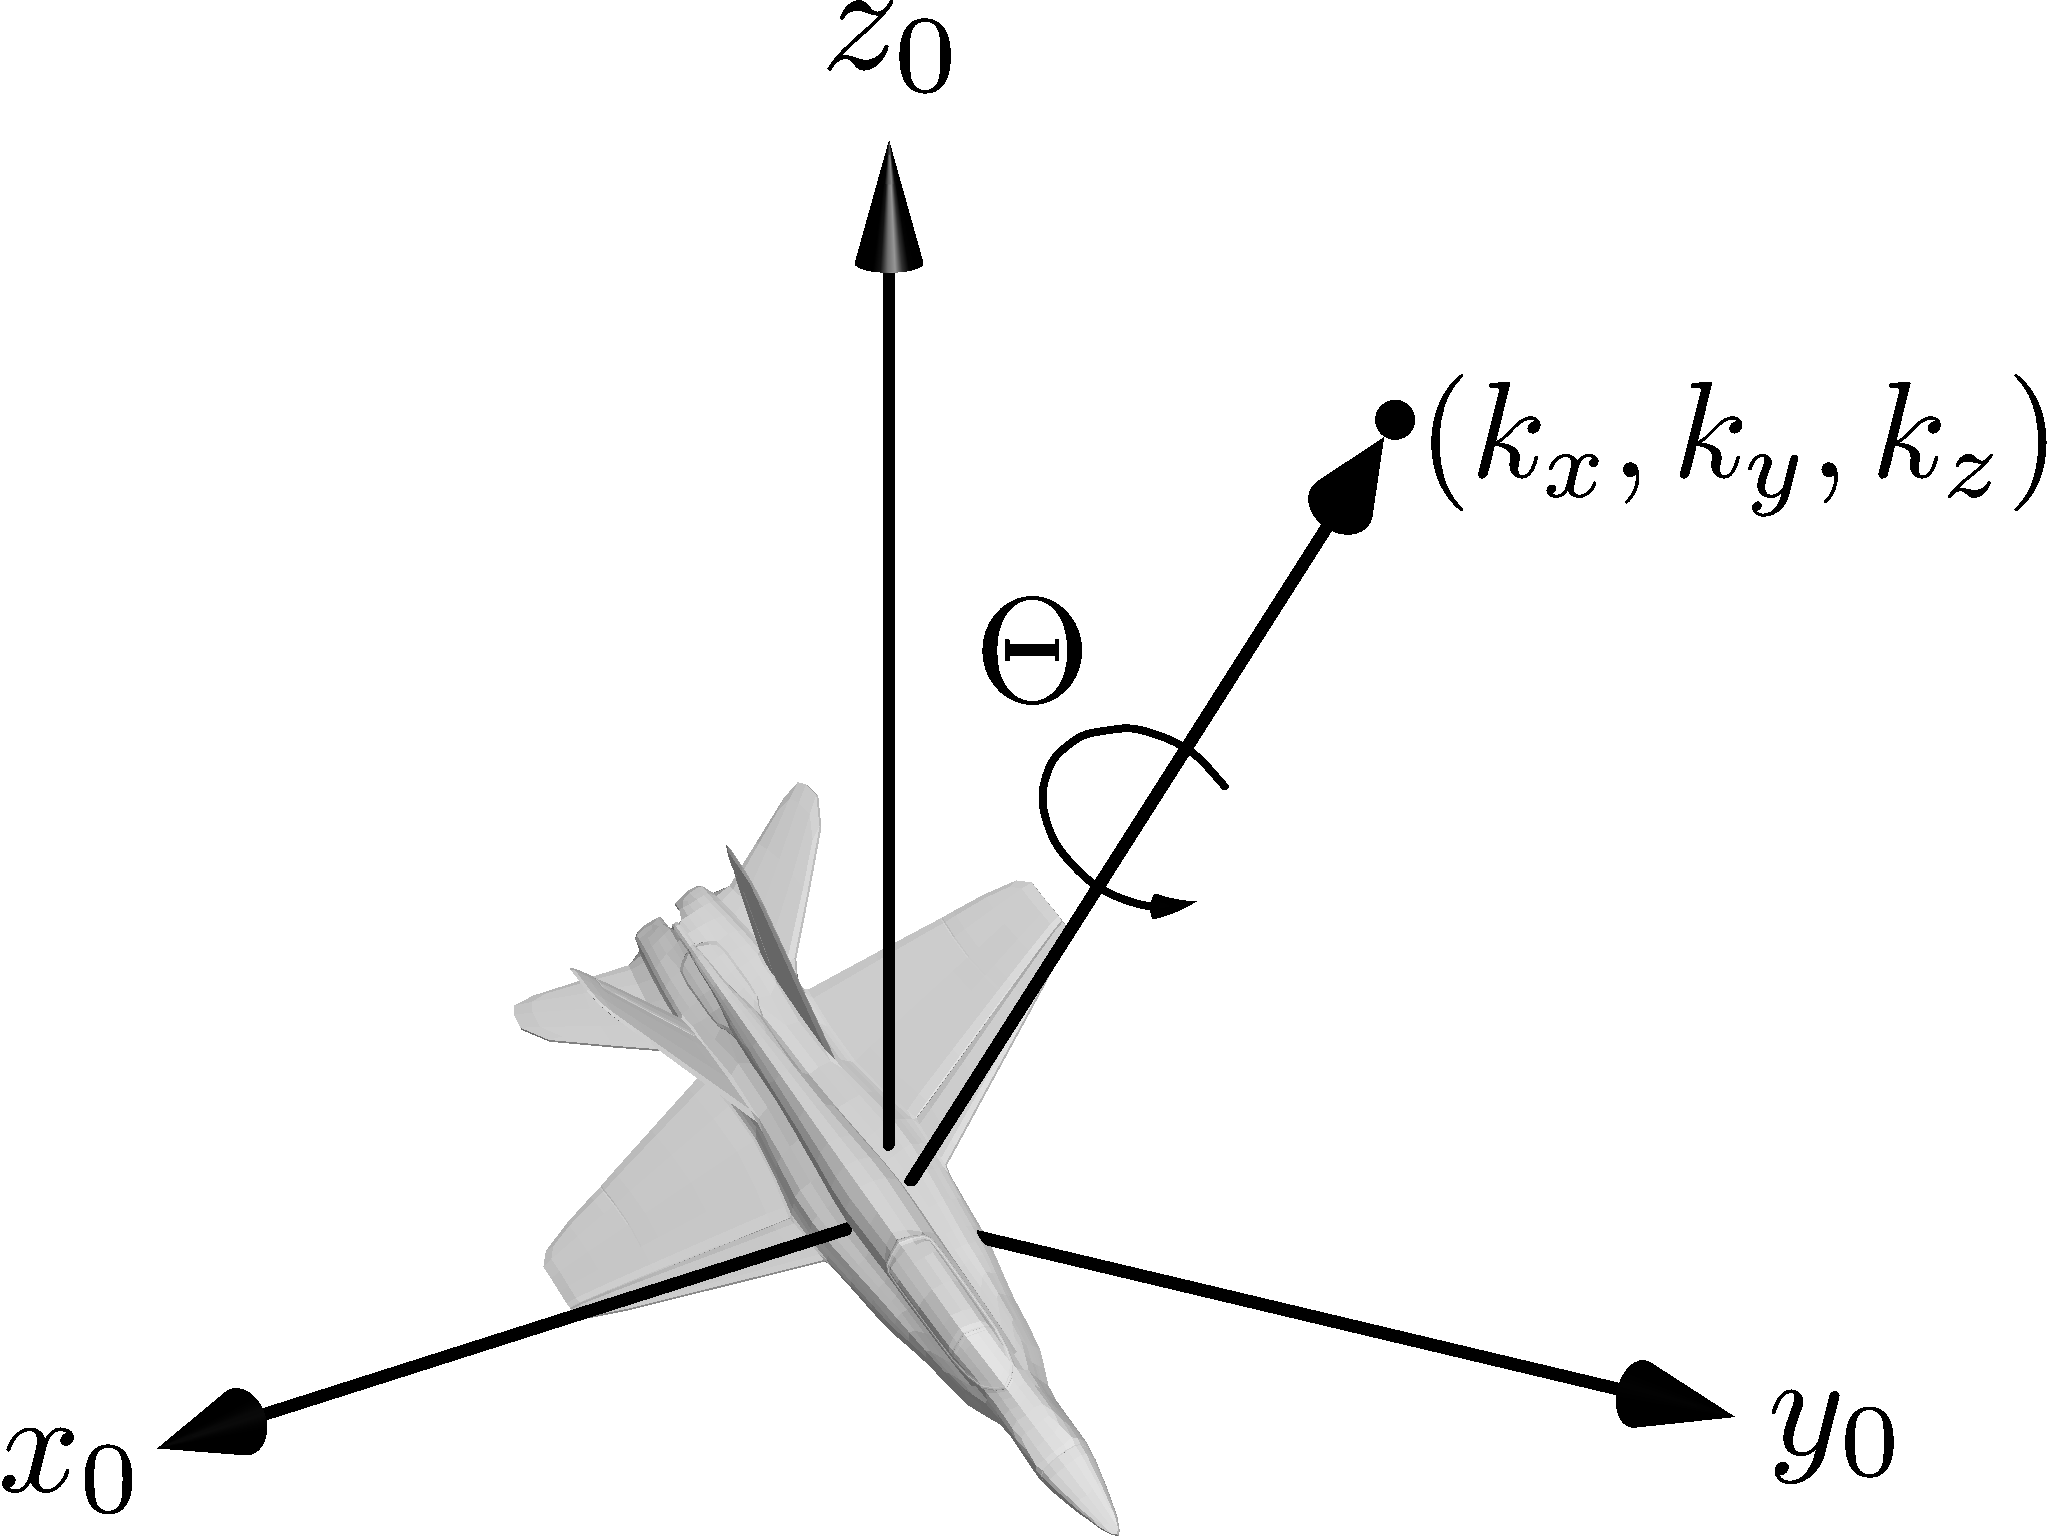
\includegraphics{frames/figs/axis_angle.png}};


\draw[->,thick,dashed,>=latex,gray] (2,0) -- (3.5,0);
%\draw[->,thick,dashed,>=latex] (e1.south west) -- (e2.north east);
%\draw[->,thick,dashed,>=latex] (e2.east) -- (e3.west);
\end{tikzpicture}

\end{center}
\caption{Axis-angle representation of orientation.}
\label{fig:axis_angle}
\end{figure}

Euler angles encode an orienation using three rotations around
pre-defined axes.  An alternate approach is to encode an orientation
as a \emph{single} rotation $\Theta$ around an arbitrary unit vector
$[k_x,k_y,k_z]^T$.
%define unit vector?? refer to appendix??
This is referred to as the \vocab{axis-angle} representation.  The
idea is illustrated in Figure \ref{fig:axis_angle}.

\subsection{Quaternions}

Probably the most widely used method for encoding orientation is the
\vocab{quaternion}.  There is a close relationship quaternions and the
axis-angle representation described above.  If $\Theta$ and
$[k_x,k_y,k_z]^T$ describe the axis-angle representation of an
orientation, then the quaternion represetation is a four-tuple $(x,
y, z, w)$ such that:

\begin{align} 
x =&  k_x \sin{\frac{\Theta}{2}}\label{eq:quat1}\\
y =&  k_y \sin{\frac{\Theta}{2}}\label{eq:quat2}\\
z =&  k_z \sin{\frac{\Theta}{2}}\label{eq:quat3}\\
w =& \cos{\frac{\Theta}{2}} \label{eq:quat4}
\end{align}

Notice that the $x$, $y$ and $z$ components point in the same
direction as the original axis of rotation.  A quaternion constructed
according to Equations \ref{eq:quat1}-\ref{eq:quat4} is also referred
to as a unit-quaternion because it has the property that $\sqrt{ x^2 +
  y^2 + z^2 + w^2} = 1$.

Quaternions are \emph{not} particularly intuitive or easy to
interpret. Their popularity is based on the fact that they support
efficient computation and they avoid the troublesome discontinuities
associated with Euler angles.


\subsection{Rotation Matrices}

Until now we have represented spatial coordinates as ordered triples:
$(x, y, z)$. Equivalently, we may think of points in space as
three-dimensional column vectors: $\begin{bmatrix}x& y&
  z\end{bmatrix}^T$.  This view is convenient because certain spatial
  transformations may be accomplished through matrix operations.  In
  particular, any rotation can be encoded as a $3\times3$
  \vocab{rotation matrix}.  Pre-multiplying the matrix by a point will
  have the effect of performing the desired rotation around the
  origin.

The following three matrices correspond to rotations around the $x$,
$y$, $z$ axes respectively:

\begin{samepage}
\begin{equation}
R_x(\Theta) = 
\begin{bmatrix}
1 & 0 & 0 \\
0 & \cos{\Theta} & -\sin{\Theta} \\
0 & \sin{\Theta} & \cos{\Theta} \\
\end{bmatrix}
\end{equation}

\begin{equation}
R_y(\Theta) = 
\begin{bmatrix}
 \cos{\Theta}& 0  & \sin{\Theta} \\
0 & 1 & 0 \\
-\sin{\Theta} & 0  & \cos{\Theta} \\
\end{bmatrix}
\end{equation}

\begin{equation}
R_z(\Theta) = 
\begin{bmatrix}
\cos{\Theta} & -\sin{\Theta} & 0 \\
\sin{\Theta} & \cos{\Theta} & 0 \\
0 & 0 & 1 \\
\end{bmatrix}
\end{equation}
\end{samepage}

Figure \ref{fig:example_matrix} shows the example of rotating the
point $\begin{bmatrix}1& 0& 0\end{bmatrix}^T$ by $90^o$ around the
  $z$-axis.

\begin{figure}
\begin{minipage}{.25\textwidth}
  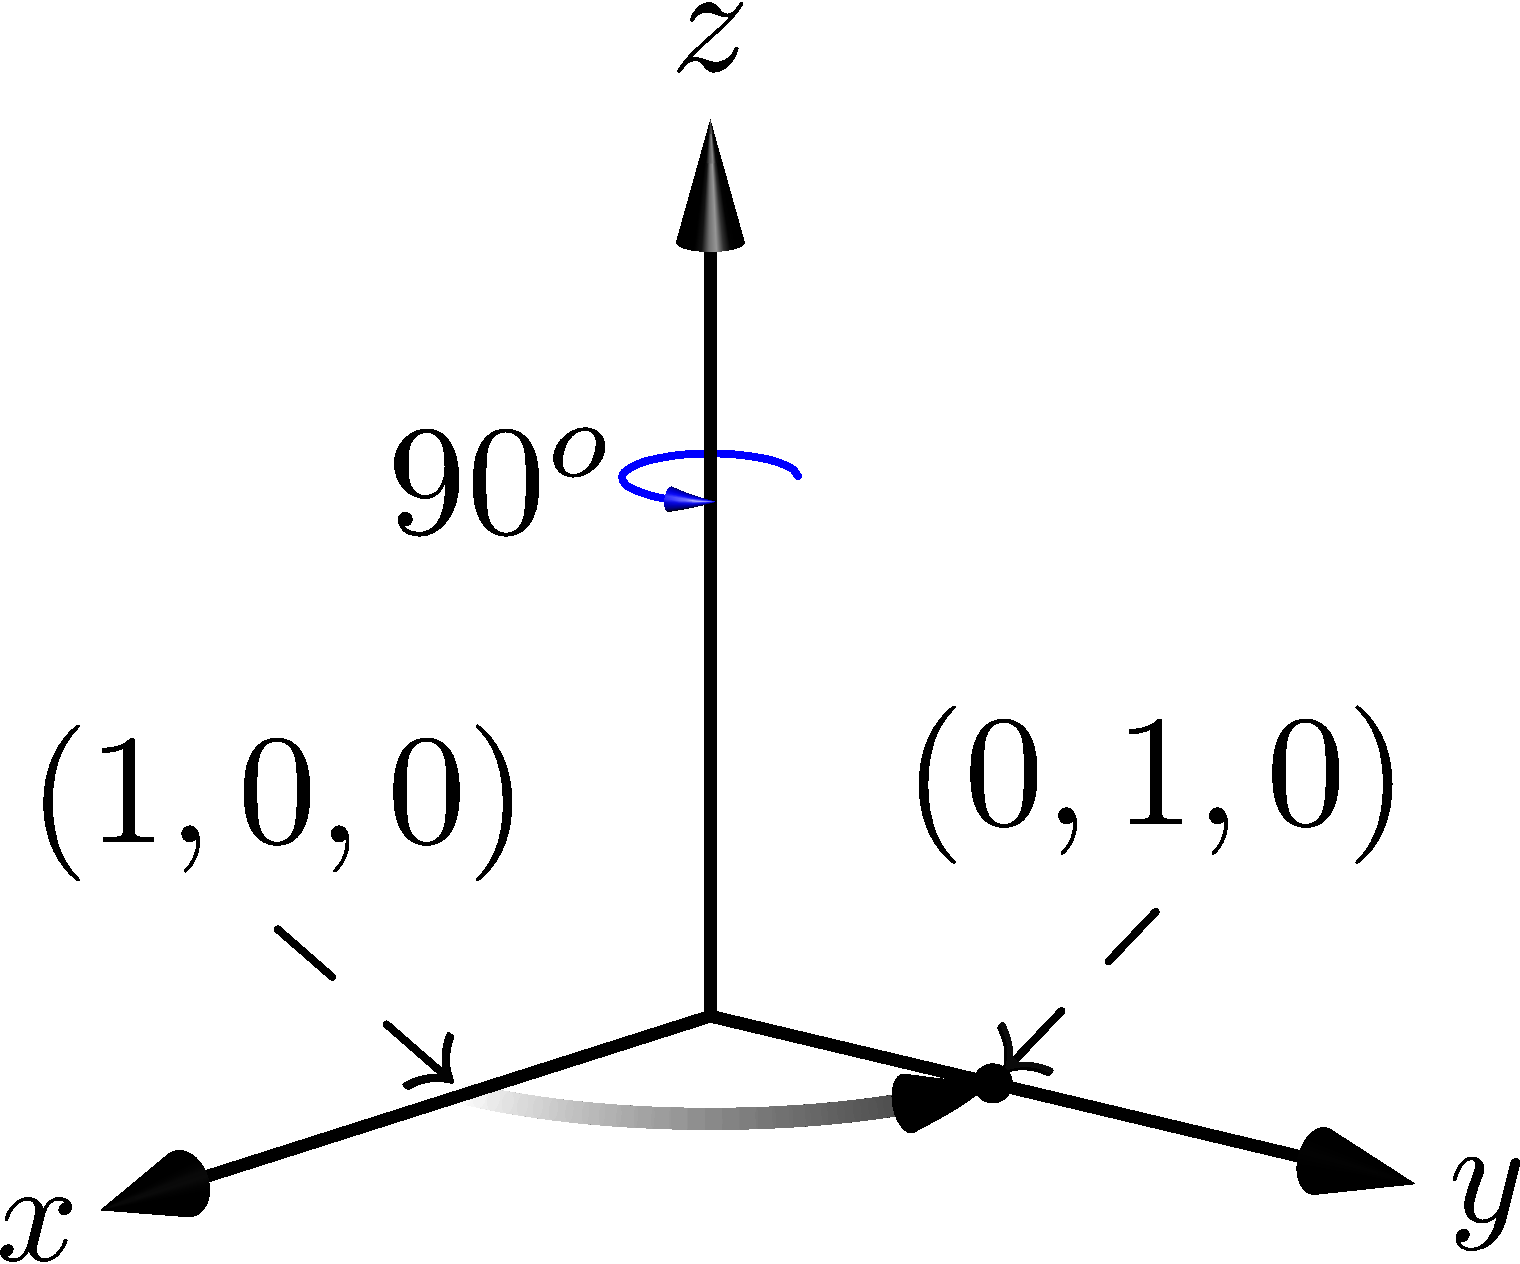
\includegraphics[]{frames/figs/rot_matrix.png}
  \end{minipage}%
  \begin{minipage}{.75\textwidth}


\begin{align*}
R_z(90^o) \times 
\begin{bmatrix}
1\\
 0\\
 0
\end{bmatrix} &=
\begin{bmatrix}
\cos{90^o} & -\sin{90^o} & 0 \\
\sin{90^o} & \cos{90^o} & 0 \\
0 & 0 & 1 \\
\end{bmatrix}
\times 
\begin{bmatrix}
1\\
 0\\
 0
\end{bmatrix} \\
&=
\begin{bmatrix}
0 & -1 & 0\\
1 & 0 & 0 \\
0 & 0 & 1 \\
\end{bmatrix}\times 
\begin{bmatrix}
1 \\
 0\\
 0
\end{bmatrix}\\
&=
\begin{bmatrix}0\\
 1\\
 0
\end{bmatrix}
\end{align*}
\end{minipage}
\caption{Example rotation}
\label{fig:example_matrix}
\end{figure}



It is possible to represent any orienation as a product of three
rotation matrices around the $x$, $y$ and $z$ axes.  It is
straightforward to convert from an Euler angle representation to the
corresponding rotation matrix.  For static rotations, the three
elementary rotation matrices must be multiplied in the order that the
rotations should be applied.  This means that the rotation matrix that
corresponds to the Euler angle rotations illustrated in Figure
\ref{fig:static_rotations} would be:

\[ R_{static} = R_x(45^o) \times R_y(30^o) \times R_z(75^o)  
\]

For Euler angles represented using relative rotations, the order is
reversed.  The rotation matrix corresponding to Figure
\ref{fig:nonstatic_rotations} would be:

\[ R_{relative} = R_z(75^o) \times R_y(30^o) \times  R_x(45^o) 
\]

The main advantage of rotation matrices is that they provide a
convenient mechasism for composing rotations and for applying
rotations to a point.  The downside is that this is a highly redundant
represenatation.  A $3\times3$ rotation matrix contains 9 values, but
as we saw in Section \ref{sec:euler} three numbers are sufficient to
represent any orientation in a three dimensional space.


\section{References and Further Reading}

Jennifer Kay provides an excellent and very accessible tutorial on
kinematics and coordinate transforms in \parencite{kay2020}.  That
tutorial also describes \vocab{homogeneous coordinates} which provide a
convenient mechanism for combining rotations and translations into a
single matrix product.

A widely used open-source software library for managing coordinate
frames and performing coordinate transforms is tf/tf2
(\url{http://wiki.ros.org/tf2}).  The tf2 library tracks time-stamped
information about the relative positions and orientations of a tree of
coordinate frames and supports efficient transforms between any two
frames. Introducing a time dimension is valuable because robots move
over time and must interact with dynamic environments. The design and
implementation of the tf library is described in \parencite{foote13}.


%% \subsection{Homogenous Transforms}

%% Recall that our goal is to be able to transform points and poses
%% between coordinate frames that are separated from each other through
%% some combination of translations and rotations.  As we saw in Section
%% \ref{sec:tranlations}  transformations are straightforward as long
%% as the coordinate frames are only separated by pure translations.

%% The method of \vocab{homogenous transforms} provides a convenient
%% mechanism for for performing transformations between \emph{any} two
%% coordinate frames.  Any combination of translations and rotations can
%% be be accomplished through a single matrix multiplication.

%% \vocab{Rotation matrices} may be used to 




% Exercises... Which of the following are right-handed?  Which are left-handed?





%\include{kinematics}

\chapter{Path Planning}
\label{chap:planning}


Chapter \ref{chap:pid} explored the problem of selecting a control
signal to drive a one-dimensional system into a desired goal state.
This Chapter will explore the more general problem of controlling
multi-dimensional systems in the presence of obstacles.

Broadly speaking, control algorithms can be broken into two
categories: \vocab{reactive} and \vocab{planning-based}.  In a
reactive system the control signal is determined solely by comparing
the current state of the system to the goal configuration. The PID
controller introduced in Chapter \ref{chap:pid} is an example of a reactive
controller.

In contrast, planning-based controllers explicitly search for a
sequence of steps that will move the state of the system into a goal
configuration. Planning-based control tends to be more appropriate in
constrained control problems such as navigating in the presence of
obstacles.  In these scenarios a reactive controller may drive the
system into a dead end, where a planning-based controller is able to
look ahead to avoid actions that won't lead to the goal.  This chapter
will focus on planning-based controllers.


\section{Configuration Spaces}

Robots come in all shapes and sizes, from tiny puck-shaped robots to
humanoid robots with dozens of degrees of freedom.
\vocab{Configuration Spaces} provide a common framework for expressing
the state of a robot within its environment.  A robot's configuration
$\mathbf{q}$ is a vector that contains all of the information
necessary to completely specify the location of a robot and all of its
constituent parts.  For the locomotive robot from Chapter \ref{chap:pid},
$\mathbf{q}$ would be a single scalar value indicating the robot's
location on the tracks.  For a humanoid robot, $\mathbf{q}$ would
include all of the robot's joint angles as well as the robot's
position and orientation within its workspace.  The full space of
possible configurations is referred to as the robot's
\vocab{Configuration Space} or \vocab{C-space} and is expressed as
$\mathbf{q} \in \mathcal{C}$.

While $\mathbf{q}$ may be high-dimensional, the world that the robot
inhabits, $\mathcal{W}$, has only three spatial dimensions (or two if
we are considering a planar path-planning problem). The mapping from a
configuration $\mathbf{q}$ to the region of space occupied by a robot is
denoted $\mathcal{A}(\mathbf{q}) \subset \mathcal{W}$ where
$\mathcal{W}=\mathbb{R}^3$ or $\mathcal{W}=\mathbb{R}^2$.


In most workspaces there will be configurations that are impossible
because they would place some part of the robot inside an obstacle. We
can denote the region of space occupied by obstacles as $\mathcal{O}
\subset \mathcal{W}$.  For the purposes of planning it is useful to
map these obstacles into the configuration space of the robot.  The
result is called the \vocab{C-space obstacle region}
$\mathcal{C}_{obs}$ and can be expressed as $\mathcal{C}_{obs} =
\{\mathbf{q} \in \mathcal{C} \mid \mathcal{A}(\mathbf{q}) \cap
\mathcal{O} \neq \emptyset\}$.  The unobstructed portion of of the
configuration space is denoted $\mathcal{C}_{free}$ where
$\mathcal{C}_{free} = \mathcal{C} - \mathcal{C}_{obs}$.

\begin{figure}
\begin{center}
\fbox{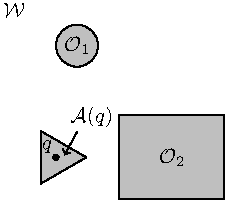
\includegraphics[]{planning/figs/workspace.pdf}}
\end{center}
\caption{Example of a triangular robot in a planar environment.}
\label{fig:workspace}
\end{figure}

Figure \ref{fig:workspace} provides an example of a triangular robot
in a two-dimensional workspace containing two obstacles. This robot
may translate within the workspace but may not rotate.  This example is
atypical in that both $\mathcal{W}$ and $\mathcal{C}$ are
two-dimensional.  If we allowed the robot to rotate,
$\mathbf{\mathbf{q}}$ would require an additional dimension to
represent the robot's orientation.  The resulting configuration space
would be expressed as $\mathcal{C} = \mathbb{R}^2 \times
\mathbb{S}^1$, where $\mathbb{S}$ represents the set of real-valued
numbers representing an angle or a point on a circle.  If we were to
additional appendages to the robot, like a trailer and an articulated
arm, the dimensionality of $\mathcal{C}$ would increase still more.


\begin{figure}
\begin{center}
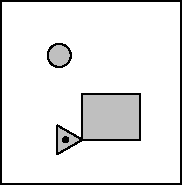
\includegraphics[]{planning/figs/pg_0001.pdf} \hspace{1em}
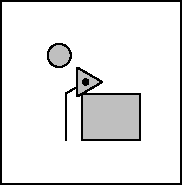
\includegraphics[]{planning/figs/pg_0003.pdf}\hspace{1em}
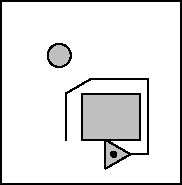
\includegraphics[]{planning/figs/pg_0008.pdf}

\vspace{1em}

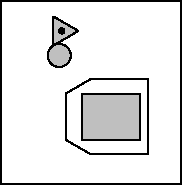
\includegraphics[]{planning/figs/pg_0010.pdf}\hspace{1em}
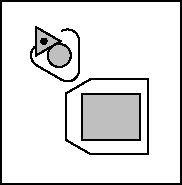
\includegraphics[]{planning/figs/pg_0014.pdf}\hspace{1em}
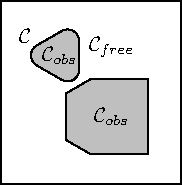
\includegraphics[]{planning/figs/pg_0015.pdf}
\end{center}
\caption{Determining $\mathcal{C}_{obs}$.  The bottom-right figure
  illustrates $\mathcal{C}_{obs}$ and $\mathcal{C}_{free}$ for the
  environment shown in Figure \ref{fig:workspace}.}
\label{fig:c_obs}
\end{figure}

Figure \ref{fig:c_obs} illustrates the relationship between the shape
of the robot, the locations of the obstacles and $\mathcal{C}_{obs}$.
In this case, we can imagine determining $\mathcal{C}_{obs}$ by tracking
$\mathbf{q}$ as we slide the robot around the boundaries of the two
obstacles.


The example in Figure \ref{fig:c_obs} is only intended to illustrate
the relationship between $\mathcal{A}(\mathbf{q})$ and
$\mathcal{C}_{obs}$.  It doesn't represent a general algorithm for
solving the problem. The problem of determining $\mathcal{C}_{obs}$
for arbitrary robots and obstacle shapes is not straightforward,
particularly in higher-dimensional configuration spaces.  In practice,
we don't typically attempt to calculate $\mathcal{C}_{free}$ before
searching for a plan.  It is usually more computationally efficient to
check configurations as-needed when they arise during the planning
process.

One shortcut for approximating $\mathcal{C}_{obs}$ is to represent
both obstacles and $\mathcal{A}(\mathbf{q})$ as spheres, or as sets of
spheres.  As long as the spheres are large enough to completely
enclose the objects, any non-overlapping configuration is guaranteed
to be in $\mathcal{C}_{free}$. This reduces collision detection to the
problem of calculating distances between object centers.

% Exercise?? draw circular approximation of C_free

Figure \ref{fig:arm} provides a second example of a robot and the
corresponding configuration space.  This is a planar two-link
articulated arm. For this robot $\mathcal{C} = \mathbb{S}^2$.


\begin{figure}
  \begin{center}  
    \begin{subfigure}[]{0.45\textwidth}
      \begin{center}
        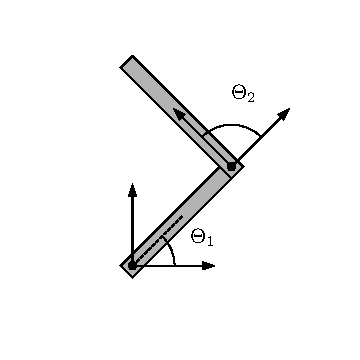
\includegraphics[]{planning/figs/arm_cspace/arm_diagram.pdf}
      \end{center}
      \caption{2D robot arm with two degrees of freedom.  For this robot
        $\mathbf{q} = [\Theta_1, \Theta_2]^T$.}
    \end{subfigure} \hspace{1em}
    \begin{subfigure}[]{0.45\textwidth}
      \begin{center}  
        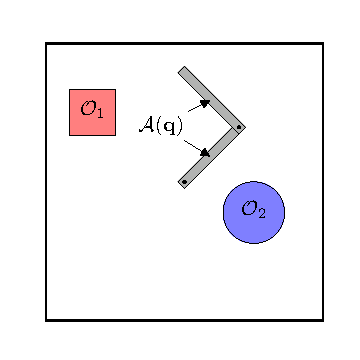
\includegraphics[]{planning/figs/arm_cspace/arm_world.pdf}
      \end{center}  
      \caption{An example of a possible configuration of the arm along
        with a pair of obstacles. Notice that $\mathcal{O}_2$ is close
        enough to the arm to prevent the first link one from making a
        full rotation.}
      \label{fig:arm_world}
    \end{subfigure}
    
    
    \begin{subfigure}[]{0.45\textwidth}
      \begin{center}  
        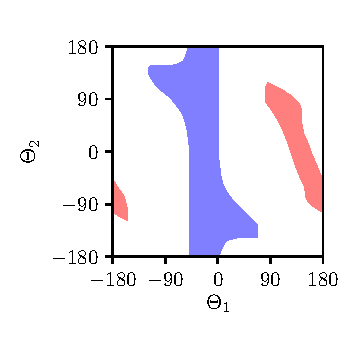
\includegraphics[]{planning/figs/arm_cspace/arm_c_space.pdf}
      \end{center}  
      \caption{An illustration of $\mathcal{C}_{obs}$ for the robot
        configuration illustrated in \ref{fig:arm_world}. The colors
        indicate configurations that intersect with the corresponding
        objects in  \ref{fig:arm_world}. }
      \label{fig:arm_c_space}
    \end{subfigure}\hspace{1em}
    \begin{subfigure}[]{0.45\textwidth}
      \begin{center}  
        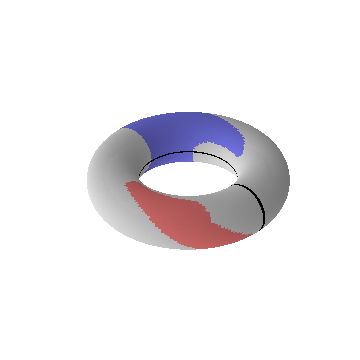
\includegraphics[]{planning/figs/arm_cspace/arm_torus.pdf}
      \end{center}  
      \caption{The configuration space from \ref{fig:arm_c_space}
        represented as a torus.  The black lines are located at
        $\theta_1 = 180/-180$ and $\theta_2 = 180/-180$.  We could
        imagine creating \ref{fig:arm_c_space} by cutting along these
        lines and unwrapping the surface. }
    \end{subfigure}
    
  \end{center}
  \caption{Configuration space visualizations for a planar two-link
    robot arm.}
  \label{fig:arm}
\end{figure}





\subsubsection*{Summary of Notation}

\begin{itemize}
  \item $\mathcal{W}=\mathbb{R}^3$ (or $\mathcal{W}=\mathbb{R}^3$) -
    The workspace containing the robot
  \item $\mathbf{q}$ - The robot's configuration
  \item $\mathcal{C}$ - The robot's configuration space
  \item $\mathcal{A}(\mathbf{q}) \subset \mathcal{W}$ - The region of space
    occupied by robot $\mathcal{A}$ in configuration $\mathbf{q}$
  \item $\mathcal{O} \subset \mathcal{W}$ - The region of space
    occupied by obstacles
  \item $\mathcal{C}_{obs}$ - The subset of the configuration space
     that is unreachable because it involves the robot intersecting with an
     obstacle.
  \item $\mathcal{C}_{free}$ - The subset of the configuration space that is
    accessible to the robot
\end{itemize}


\subsection{The Path Planning Problem}



\begin{figure}
\begin{center}
  \includegraphics[]{planning/figs/path_c_obs.pdf}
  \includegraphics[]{planning/figs/path_world.pdf}
\end{center}
\caption{Left: A valid path from an initial configuration
  $\mathbf{q}_{I}$ to a goal configuration $\mathbf{q}_{G}$. Right:
  The robot trajectory corresponding to the indicated path. }
\label{fig:path_triangle}
\end{figure}

\begin{figure}
  \begin{center}

      \includegraphics[valign=t]{planning/figs/arm_cspace/arm_c_space_motion.pdf}
      \includegraphics[valign=t]{planning/figs/arm_cspace/arm_world_motion.pdf}

\end{center}
\caption{Left: A valid path from an initial configuration
  $\mathbf{q}_{I}$ to a goal configuration $\mathbf{q}_{G}$. Right:
  The robot trajectory corresponding to the indicated path. }
\label{fig:path_arm}
\end{figure}



Once $\mathcal{C}_{free}$ is determined, the path-planning problem is
conceptually simple.  All we need to do is find a continuous path in
$\mathcal{C}_{free}$ from some starting configuration $\mathbf{q}_{I}$
to the goal configuration $\mathbf{q}_{G}$.  This standard formulation
(sometimes called \vocab{the piano movers problem}) allows us to avoid
re-thinking the path planning problem for each new robot or
environment.  All of robotic path planning boils down to finding a
path from one point to another within a known subset of some
(potentially high-dimensional) space.  Figures \ref{fig:path_triangle}
and \ref{fig:path_arm} show examples of valid paths for the triangle
robot and the two-link arm respectively.


%% EXERCISES:
%% Consider the 2d triangular robot below.  C-space is $R^2$.  Draw $A(\mathbf{q})$ for
%% \mathbf{q} = (2,3), \mathbf{q}=(0,0)

%% Now consider these obstacles:
%% Draw C_{obs}

%% Cart pole $R^1 \times S^1$
%% Repeat above


\subsection{Constraints}

The discussion above assumes that any robot configuration is allowed,
as long as the robot doesn't intersect with an obstacle. In practice,
there are often additional constraints on the set of possible
configurations. These constraints can be classified as
\vocab{holonomic} or \vocab{non-holonomic}.

\subsubsection{Holonomic Constraints}

Holonomic constraints result from physical restrictions that make it
impossible for the robot to enter some regions of the configuration
space.  For example, the elbow joint on a robotic arm may only have a
90 degree range of motion.  Holonomic constraints don't significantly
complicate the path planning problem: we can simply extend our notion
of $\mathcal{C}_{free}$ to exclude restricted regions.

\subsubsection{Non-Holonomic Constraints}

Non-holonomic constraints don't directly restrict which regions of the
space are accessible. Instead, they restrict how the robot can move
from one configuration to another.  A classic example of a
non-holonomic constraint is the inability of a car to slide sideways
into a parking spot.  There is no constraint preventing the car from
being in the parking spot, but the mechanics of the vehicle prevent it
from following a straight-line path to the desired configuration.
Non-holonomic constraints can also arise from system dynamics: A
vehicle moving at 5 miles per hour can easily make a 30 degree turn,
while a vehicle moving at 50 miles per hour would roll over.
Non-holonomic constraints of this sort are referred to as
\vocab{kino-dynamic constraints}.  Non-holonomic constraints
complicate the path planning problem and require the use of
specialized algorithms.


% Thought questions....
\subsection*{Stop and Think}

\begin{exercise}
  Draw  $\mathcal{C}_{free}$ and $\mathcal{C}_{obs}$ for the world pictured below:

  \begin{center}
\fbox{\includegraphics[]{planning/figs/exercises/workspace_hw.pdf}}
\end{center}
  
  Assume that this is the same non-rotating triangular robot
  illustrated in Figures \ref{fig:workspace} and \ref{fig:c_obs}.
\end{exercise}

\begin{exercise}

  The robot in Figure \ref{fig:workspace} has a configuration space
  that can be expressed as $\mathcal{C} = \mathbb{R}^2$, the robot in
  Figure \ref{fig:arm} had a configuration space expressed as
  $\mathcal{C} = \mathbb{S}^2$.  Imagine a more complex robot that
  combines attributes of these two examples.  This new robot is a
  triangle robot that is able to translate, rotate in place, and is
  equipped with a two-link robotic arm.  How many degrees of freedom
  does this robot have?  How would we express configuration space for
  this robot?
  %(R^2 x S^3)
\end{exercise}

\begin{exercise}
Some configurations of a robotic arm may be impossible because of
self-collisions.  Is this an example of a holonomic or a
  non-holonomic constraint?
\end{exercise}

\begin{exercise}
In the text above we used set-builder notation to express the
C-obstacle region as as $\mathcal{C}_{obs} = \{\mathbf{q} \in
\mathcal{C} \mid \mathcal{A}(\mathbf{q}) \cap \mathcal{O} \neq
\emptyset\}$, where $\mathcal{O}$ represents the subset of
$\mathcal{W}$ occupied by obstacles.  What set of configurations are represented by  $\{\mathbf{q} \in
\mathcal{C} \mid ( \mathcal{A}(\mathbf{q}) \cup \mathcal{O}) \subseteq
\mathcal{O}\}$?
  \end{exercise}

\section{Planning Algorithms}

The general path planning problem outlined above is conceptually
simple but computationally difficult.  Path planning has been shown to
be PSPACE-Hard, making it extremely unlikely that we will ever have a
polynomial time algorithm that is guaranteed to find a path if one
exists.  This means that practical planning algorithms necessarily
involve compromises in completeness or involve attacking simplified
versions of the problem.  The remainder of this chapter will explore
several approaches to planning.


\section{Grid-Based Search}
\label{sec:graph_search}


\begin{figure}
\begin{center}
\includegraphics[]{planning/figs/grid1.pdf} \hspace{1em}
\includegraphics[]{planning/figs/grid2.pdf} \hspace{1em}
\includegraphics[]{planning/figs/grid3.pdf}
\end{center}
\caption{Discretizing the configuration space.  The figure on the left
  shows a uniform grid overlaying the configuration space.  In the
  center figure, all grid cells that overlap with $\mathcal{C}_{obs}$
  have been marked as inaccessible.  The figure on the right shows the
  state space graph that results if all accessible cells are connected
  to their neighbors. }
\label{fig:discretization}
\end{figure}


One way to simplify the planning problem is to perform a uniform
discretization of the configuration space and the space of possible
actions.  For example, it is common to handle holonomic 2D navigation
problems by overlaying the 2D configuration space with a grid.  Actions
are restricted to moving between four-connected or eight-connected
grid cells.  Figure \ref{fig:discretization} illustrates one possible
discretization of the triangle-robot configuration space described in
the previous section.  The result is a graph where the vertices
represent states and the edges represent actions.

Notice that the discretization in Figure \ref{fig:discretization}
makes it impossible for the robot to find a path that passes between
the two obstacles.  This highlights a trade-off between the
granularity of the discretization and the quality of the possible
solutions.  We can make our discretization arbitrarily close to the
continuous version of the problem by reducing the granularity, but
finer discretizations come at the cost of more grid cells which
increases the cost of planning.


\begin{listing}[H]
\begin{minted}[mathescape,linenos,
               fontsize=\small,
               frame=single,
               framesep=2mm]{python}

def search(problem):
    """
    Args:
        problem: a problem instance that provides three methods:

              problem.start() -       returns the start state
              problem.goal()  -       returns the goal state
              problem.successors(s) - returns the states that are 
                                      adjacent to s

    Returns:                              
        True if there exists a sequence of states leading from
        problem.start() to problem.goal(), or False if no such
        path exists
    """
    
    frontier = Collection()  # The collection of states that are
                             # currently eligible for expansion         
             
    closed = set()           # The set of states that have already
                             # been expanded

    frontier.add(problem.start())  # Initialize the search by adding
                                   # the start state to the frontier

    while not frontier.is_empty():
        cur_state = frontier.pop()  # Select the next eligible state
                                    # to expand

        closed.add(cur_state)       # Make sure that this state can't 
                                    # be added to the frontier again

        if cur_state == problem.goal():  # Success!
            return True
        
        else:
            # Add the neighbors of the selected state to the frontier...
            for next_state in problem.successors(cur_state):
                if (next_state not in closed and
                        next_state not in frontier):
                    frontier.add(next_state)
                        
    return False   # No path was found!

\end{minted}
\caption{Basic graph search algorithm.}
\label{lst:graph_search}
\end{listing}

Once a search problem has been formulated as a graph, we can use
standard graph-search algorithms to find a permissible path to the
goal.  Listing \ref{lst:graph_search} presents the basic graph search
algorithm. The algorithm works outward from the start state,
maintaining a collection of states on the frontier of the region we
have already searched.  At each iteration, we select a state from the
frontier and add its neighbors back into the frontier.  This process
continues until the goal state is selected from the frontier.

Selecting and processing a state from the frontier is referred to as
\emph{expansion}. Maintaining a \emph{closed set} allows us to avoid
re-processing states that have already been expanded.  Each time a
state is expanded it is added to the closed set.  Once a state is
closed, the check on line 39 ensures that it will never be added back
into the frontier.  This check prevents the algorithm from considering
paths containing cycles.

The collection type used to store the frontier determines the order
that the states are expanded during search.  When a queue is used, the
algorithm in Listing \ref{lst:graph_search} performs a
breadth-first-search (BFS), while the use of a stack results in
depth-first-search (DFS).

For search problems with uniform step costs, BFS is both
\vocab{complete} and \vocab{optimal}.  A complete search algorithm is
guaranteed to find a path if one exists.  An optimal search algorithm
is guaranteed to find the lowest-cost path.  BFS is optimal in the
sense that it is guaranteed to find the path with the fewest possible
steps.  By storing the frontier in a FIFO queue we ensure that all
paths of length $n$ are explored before we explore any paths of length
$n+1$.

In contrast, DFS is neither complete nor optimal. In the case of
an infinite graph, DFS could potentially perform infinite expansions
away from the goal state, even if the goal could be reached within only a
small number of steps.  The advantage of DFS is that it requires less
memory to store the frontier.  The number of nodes in the frontier
grows linearly for DFS but it may grow exponentially for BFS,
depending on the structure of the search problem.


\begin{figure}
  \begin{center}
    \begin{subfigure}[t]{0.3\textwidth}
      \includegraphics[width=1.25in]{planning/figs/bfs_0001.pdf}
       \caption{One expansion}
    \end{subfigure}
    \begin{subfigure}[t]{0.3\textwidth}
      \includegraphics[width=1.25in]{planning/figs/bfs_0002.pdf}
       \caption{Two expansions}
    \end{subfigure}
    \begin{subfigure}[t]{0.3\textwidth}
      \includegraphics[width=1.25in]{planning/figs/bfs_0009.pdf}
       \caption{Nine expansions}
    \end{subfigure}

    \vspace{.2in}

    \begin{subfigure}[t]{0.3\textwidth}
      \includegraphics[width=1.25in]{planning/figs/bfs_0081.pdf}
       \caption{81 expansions}
    \end{subfigure}
    \begin{subfigure}[t]{0.3\textwidth}
      \includegraphics[width=1.25in]{planning/figs/bfs_0350.pdf}
       \caption{350 expansions}
    \end{subfigure}
    \begin{subfigure}[t]{0.3\textwidth}
      \includegraphics[width=1.25in]{planning/figs/bfs_0641.pdf}
       \caption{641 expansion}
    \end{subfigure}

\end{center}
  \caption{BFS search example.  The cell containing the start state is
    colored green and the goal state is colored gold. States in the
    frontier are shown in blue.  States in the closed set are shown in
    gray.  The final path is shown in red. }
\label{fig:bfs}
\end{figure}




\begin{figure}
  \begin{center}
    \begin{subfigure}[t]{0.3\textwidth}
      \includegraphics[width=1.25in]{planning/figs/dfs_0001.pdf}
       \caption{One expansion}
    \end{subfigure}
    \begin{subfigure}[t]{0.3\textwidth}
      \includegraphics[width=1.25in]{planning/figs/dfs_0002.pdf}
       \caption{Two expansions}
    \end{subfigure}
    \begin{subfigure}[t]{0.3\textwidth}
      \includegraphics[width=1.25in]{planning/figs/dfs_0009.pdf}
       \caption{Nine expansions}
    \end{subfigure}

    \vspace{.2in}

    \begin{subfigure}[t]{0.3\textwidth}
      \includegraphics[width=1.25in]{planning/figs/dfs_0081.pdf}
       \caption{81 expansions}
    \end{subfigure}
    \begin{subfigure}[t]{0.3\textwidth}
      \includegraphics[width=1.25in]{planning/figs/dfs_0350.pdf}
       \caption{350 expansions}
    \end{subfigure}
    \begin{subfigure}[t]{0.3\textwidth}
      \includegraphics[width=1.25in]{planning/figs/dfs_0477.pdf}
       \caption{477 expansion}
    \end{subfigure}

\end{center}
\caption{DFS search example.}
\label{fig:dfs}
\end{figure}


Figure \ref{fig:bfs} illustrates a BFS search in our triangle-world
workspace.  Figure \ref{fig:dfs} illustrates a DFS search.


\subsection{Returning A Path}

The careful reader will notice that the algorithm in Listing
\ref{lst:graph_search} doesn't actually return a path to the goal.  It
only determines whether such a path exists.  In order to reconstruct
the path we need to maintain an auxiliary data structure that stores
backward references from each state to the state that precedes it.
Once the goal is reached, the path can be reconstructed by following
the backward references from the goal back to the start state and then
reversing the steps.  Listing \ref{lst:node_search} shows a possible
Python implementation of the necessary data type and an appropriately
updated version of the algorithm from Listing \ref{lst:graph_search}.

The containment check on line 40 of Listing \ref{lst:node_search}
requires some clarification.  The goal here is to avoid exploring
multiple paths that pass through the same state.  If the frontier
already contains a node for a state, we don't want to add another node
that represents a different route to that state.  This means that the
test on line 40 is \emph{not} checking to see if the indicated Node is
in the frontier, it is checking to see if any Node in the frontier
contains \mintinline {python}{new_state}.  Removing this check would
not impact the correctness of the algorithm, but it would
significantly impact efficiency for problems that allow many different
paths to each state.


\definecolor{ly}{RGB}{255, 255, 200}
\begin{listing}[H]
  \begin{minted}[mathescape,linenos,
      escapeinside=||,
               fontsize=\small,
               frame=single,
               framesep=2mm]{python}
|\colorbox{ly}{class Node:}|
    """The Node class stores backward references from each state
       encountered in the search to a Node representing the
       state that preceded it.
    """    
    def __init__(self, state, parent_node):
        self.state = state
        self.parent = parent_node


def search(problem):
    """
    Input: problem - a problem instance that provides three methods:

              problem.start() -       returns the start state
              problem.goal()  -       returns the goal state
              problem.successors(s) - returns the states that are 
                                      adjacent to s

    Returns: A sequence of states leading from problem.start() to 
             problem.goal(), or None if no path exists
    """
    frontier = Collection()
    closed = set()

    frontier.add(|\colorbox{ly}{Node(problem.start(), None)}|)    

    while not frontier.is_empty():
        |\colorbox{ly}{cur\_node}| = frontier.pop()
        |\colorbox{ly}{cur\_state = cur\_node.state}|
        closed.add(cur_state)

        if cur_state == problem.goal():
            return |\colorbox{ly}{construct\_path(cur\_node)}| # path ending at this node
        
        else:
            for next_state in problem.successors(cur_state):
                |\colorbox{ly}{next\_node = Node(next\_state, cur\_node)}|
                if (next_state not in closed and
                        |\colorbox{ly}{next\_node}| not in frontier): # See text.
                    frontier.add(|\colorbox{ly}{next\_node}|)

    return |\colorbox{ly}{None}|

\end{minted}
\caption{Graph search algorithm updated to return a path.  Steps that
  differ from Listing \ref{lst:graph_search} are highlighted in
  yellow.  The key difference is that the frontier stores Node objects
  rather than states.}
\label{lst:node_search}
\end{listing}

% Thought questions:
\subsection*{Stop and Think}

\begin{exercise}
  Consider the following graph:

  \includegraphics[width=1.25in]{planning/figs/exercises/hw_graph_no_weights.pdf}
  
  Complete the table below to show the state of search algorithm
  \ref{lst:node_search} after each iteration of a DFS search starting
  at state $g$ with the goal at state $a$.  The tuples in the Frontier
  column represent Node objects where the first entry is the state and
  the second entry is the state associated with the parent node.
  Assume that the loop on line 37 accesses neighbors in
  alphabetical order.  The first three steps are completed for you.

  \begin{center}
%\def\arraystretch{1.5}%  1 is the default, change whatever you need
\begin{tabular}{|l|l|p{3in}|p{1in}|}
  \hline
  Expansions & Chosen  & Frontier & Closed Set \\
  \hline
  0 & -- & $\langle g, \text{--} \rangle$& --\\
  \hline
  1&$g$& $\langle d, g \rangle$, $\langle h, g \rangle$& \{$g$\}\\
  \hline
    3& $h$ & $\langle d, g \rangle$,  $\langle e, h \rangle$, $\langle i, h \rangle$  & \{$g, h$\} \\
    \hline
    3&&&\\
    \hline
    4&&&\\
    \hline
    5&&&\\
    \hline
    6&&&\\
    \hline
    7&&&\\
    \hline
\end{tabular}
\end{center}

  What is the final path discovered by DFS?  (You should be able to reconstruct it by working backward through the parent entries starting from the point where $a$ is selected from the frontier.)
\end{exercise}

\begin{exercise}
  Repeat the previous exercise using a BFS search.
\end{exercise}

\begin{exercise}
The algorithm in Listing \ref{lst:graph_search} is described as a
graph search algorithm, but the graph is implicit: graph edges are
essentially generated as needed through calls to \mintinline
{python}{problem.successors}. Why might this approach make more sense
than explicitly creating a complete graph structure before executing a
search?
\end{exercise}

\begin{exercise}
What if we knew that the state space being searched is actually a tree
rooted at the start state?  How would this allow us to simplify the
search algorithm in Listing \ref{lst:graph_search}?  Can you think of
a path-planning problem that would have a tree-structured search
space?
\end{exercise}

\subsection{Dijkstra's Algorithm}


\begin{listing}[H]
  \begin{minted}[mathescape, linenos,
      escapeinside=||,
               fontsize=\small,
               frame=single,
               framesep=2mm]{python}
class Node:
    def __init__(self, state, parent_node, |\colorbox{ly}{step\_cost}|):
        self.state = state
        self.parent = parent_node
        |\colorbox{ly}{self.path\_cost = parent\_node.path\_cost + step\_cost}|

def dijkstra(problem):
    frontier = |\colorbox{ly}{PriorityQueue()}|
    closed = set()

    start_node = Node(problem.start(), None, |\colorbox{ly}{0.0}|)
    frontier.add(start_node, |\colorbox{ly}{0.0}|)

    while not frontier.is_empty():
        cur_node = frontier.pop()
        cur_state = cur_node.state
        closed.add(cur_state)

        if cur_state == problem.goal():
            return construct_path(cur_node)
        else:
            for next_state in problem.successors(cur_state):
                |\colorbox{ly}{cost = problem.cost(cur\_state, next\_state)}|
                next_node = Node(next_state, cur_node, |\colorbox{ly}{cost}|)
                if next_state not in closed:
                    frontier.add(next_node, |\colorbox{ly}{next\_node.path\_cost}|)
    return None
\end{minted}
\caption{Dijkstra's algorithm.  Steps that differ from Listing
  \ref{lst:node_search} are highlighted.  The key difference is that
  the frontier is represented by a Priority Queue that is ordered by
  the total cost to reach the state.}
\label{lst:dijkstra}
\end{listing}


In many path-planning problems there is a notion of path cost that is
distinct from the number of edges in the path.  In the case of 2D
navigation, the cost of a path might be the total distance traveled,
the time required to reach the goal, or the amount of energy expended
by the robot.

For example, if we want to find shortest paths in the grid navigation
problem from Figure \ref{fig:discretization} we should assign weights
to the edges in proportion to the distance that the robot must travel
to move from cell to cell.  This means that diagonal steps must have a
higher weight to reflect the fact that the robot moves farther.  An
optimal solution to this weighted version of the problem will
represent the shortest path in terms of distance traveled.  Notice
that the path discovered by BFS in Figure \ref{fig:bfs} is optimal in
terms of the number of steps taken, but it is clearly not optimal in
terms of distance.

With some slight modification, the algorithm in Listing
\ref{lst:node_search} can be updated to take path costs into account.
Listing \ref{lst:dijkstra} shows the updated algorithm.  The main
differences are that the Node implementation has been updated to store
the total path cost required to reach the corresponding state, and the
frontier is now represented by a Priority Queue ordered by path cost.
The Priority Queue ensures that Nodes are expanded in strictly
increasing order of path cost.  Given that all edges must have
positive weights, each time an expansion occurs, all of the nodes
added back to the frontier are guaranteed to have a higher cost than
the node that was expanded.  This means that when a node representing
the goal state is expanded it must represent the lowest-cost path to
the goal.
 
Notice that the algorithm in Listing \ref{lst:dijkstra} does not check
if a state is already on the frontier before adding the new node for
that state.  From the point of view of correctness, this is fine:
There is no danger of finding a longer path to the goal before a
shorter path is discovered since the lower-cost node will be expanded
first.  However, it is more efficient to implement the frontier so
that any higher-cost node is replaced when a lower-cost node is added
for the same state.  This prevents the wasted effort of expanding a
higher-cost node (representing a longer path to the same state) after
a lower-cost node.


\begin{figure}
  \begin{center}
    \begin{subfigure}[t]{0.3\textwidth}
      \includegraphics[width=1.25in]{planning/figs/dijkstra_0001.pdf}
       \caption{One expansion}
    \end{subfigure}
    \begin{subfigure}[t]{0.3\textwidth}
      \includegraphics[width=1.25in]{planning/figs/dijkstra_0002.pdf}
       \caption{Two expansions}
    \end{subfigure}
    \begin{subfigure}[t]{0.3\textwidth}
      \includegraphics[width=1.25in]{planning/figs/dijkstra_0013.pdf}
       \caption{13 expansions}
    \end{subfigure}

    \vspace{.2in}

    \begin{subfigure}[t]{0.3\textwidth}
      \includegraphics[width=1.25in]{planning/figs/dijkstra_0100.pdf}
       \caption{100 expansions}
    \end{subfigure}
    \begin{subfigure}[t]{0.3\textwidth}
      \includegraphics[width=1.25in]{planning/figs/dijkstra_0350.pdf}
       \caption{350 expansions}
    \end{subfigure}
    \begin{subfigure}[t]{0.3\textwidth}
      \includegraphics[width=1.25in]{planning/figs/dijkstra_0674.pdf}
       \caption{674 expansion}
    \end{subfigure}



\end{center}
\caption{Dijkstra's algorithm search example}
\label{fig:dijkstra}
\end{figure}


Figure \ref{fig:dijkstra} shows an example of applying Dijkstra's
algorithm to the triangle navigation problem.  The resulting path is
optimal for the given discretization.

% Thought questions...
\subsection*{Stop and Think}

\begin{exercise}
  \label{ex:dij_table}
  Consider the following weighted graph:

  \includegraphics[width=1.25in]{planning/figs/exercises/hw_graph.pdf}
  
  Complete the table below to show the state of Dijkstra's algorithm
  after each expansion.  Again the start state is $g$ and the goal
  state is $a$.  Break priority ties using alphabetical order.
  I.e. in the case of a tie, state $a$ will selected before state
  $b$. The tuples in the Frontier column represent Node objects where
  the first entry is the state, the second entry is the state
  associated with the parent node and the third entry is the path cost
  to reach the state. The first three steps are completed for you.

  \begin{center}
%\def\arraystretch{1.5}%  1 is the default, change whatever you need
\begin{tabular}{|l|l|p{3in}|p{1in}|}
  \hline
  Expansions & Chosen  & Frontier & Closed Set \\
  \hline
  0 & -- & $\langle g, \text{--}, 0 \rangle$& --\\
  \hline
  1&$g$& $\langle d, g , 6\rangle$, $\langle h, g, 1 \rangle$& \{$g$\}\\
  \hline
    3& $h$ & $\langle d, g, 6 \rangle$,  $\langle e, h, 3 \rangle$, $\langle i, h, 2 \rangle$  & \{$g, h$\} \\
    \hline
    3&&&\\
    \hline
    4&&&\\
    \hline
    5&&&\\
    \hline
    6&&&\\
    \hline
    7&&&\\
    \hline
    8&&&\\
    \hline
\end{tabular}
\end{center}

  What final path is returned?  What is the path cost?
\end{exercise}

\begin{exercise}
  Compare \ref{fig:bfs} to \ref{fig:dijkstra}.  Why is the
  frontier more or less square in one and round in the other?
\end{exercise}

\begin{exercise}
Take a look at the true, non-discretized, configuration space from
Figure \ref{fig:workspace}.  What would the shortest path look like in
that space?  Why is it different from the path shown in figure
\ref{fig:dijkstra}?
\end{exercise}

\begin{exercise}
Is it guaranteed that there will always be a unique minimum-cost path?
If not, how could the algorithm in Listing \ref{lst:dijkstra} be
updated to return all such paths?
\end{exercise}


%% \begin{exercise}
%% Is it always the case that the shortest Euclidean distance between two
%% configurations represents the most efficient path for the robot to
%% take between those configurations?  If not, describe a
%% counter-example.
%% \end{exercise}




\subsection{A*}

All of the graph search algorithms discussed so far can be described
as \vocab{undirected}. This means that they ``blindly'' work their
way out from the start state until the goal state is encountered.
Intuitively, it seems that we should be able to search more quickly by
preferring to expand nodes that are likely to be closer to the goal:
If we know that the goal is to the east of the robot, then
surely we should start the search by exploring actions that move the
robot in that direction.

This intuition can be formalized through the idea of a
\vocab{heuristic function} $h(s)$.  A heuristic function maps from a
state to the estimated cost of reaching the goal from that state.
States with lower heuristic values are believed to be closer to the
goal, and thus should be explored before states with higher heuristic
values.

We can easily update Dijkstra's algorithm to take advantage this idea.
The only change required is that the the Priority Queue representing
the frontier will now be ordered by $f(s) = c(s) + h(s)$ where $c(s)$
represents the cost of reaching state $s$, and $h(s)$ represents the
estimated cost of reaching the goal from $s$.  The sum
represents an estimate of the overall cost of the shortest path that
passes through state $s$. The resulting Algorithm is called A*.

The A* algorithm is guaranteed to find an optimal path as long as the
heuristic function satisfies two requirements: First, it must never
overestimate the true cost of reaching the goal.  An overestimate
could prevent a node from being expanded, even if that node is on the
shortest path to the goal.  Second, the heuristic function must be
\vocab{consistent}.  Formally, this means that $h(s) \leq h(s') + cost(s,
s')$ for all states $s$ and $s'$ where $cost(s, s')$ represents the
cost of the edge between $s$ and $s'$.  Informally, this means that
the heuristic function should respect the actual step costs.  When
stepping from $s$ to $s'$, the heuristic function shouldn't drop by
more than the cost of the step.

The ``*'' in A* was chosen to indicate that this is, in a sense, the
last word in heuristic-based graph search algorithms.  Not only is A*
guaranteed to find a shortest path, it is also provably optimal in
terms of the number of nodes expanded.  Any algorithm that is
guaranteed to find a shortest path must expand at least as many nodes
as A* when using the same heuristic function.

Taking full advantage of A* requires the selection of a good heuristic
function. A good heuristic function should be as close as possible to
the true cost of reaching the goal, while being fast to compute and
satisfying the consistency requirement.  In general, it can be
challenging to satisfy these requirements.  However, in robotic path
planning problems where the objective is to find a minimum length
path, the straight-line distance to the goal is often a reasonable
choice.  The straight-line distance is easy to compute. It may
underestimate the true cost, (because it doesn't take obstacles into
account) but it can never overestimate: the straight-line distance
always represents the shortest possible path to the goal.  If the step
cost is taken to be the distance traveled, then the straight line
distance is consistent because no step can reduce the distance to the
goal by more than the distance moved.

Figure \ref{fig:astar} illustrates an A* search using the straight
line heuristic.  Notice that, while A* does not return the same path
that was discovered by Dijkstra's algorithm, the two paths have the
same length and both are optimal.

% Thought questions.
\subsection*{Stop and Think}

\begin{exercise}
  The \vocab{Manhattan distance} is a count of the minimum number of
  edges between two states in a four-connected grid.  Is Manhattan
  distance an admissible heuristic for the search problem in Question
  \ref{ex:dij_table}?
  \end{exercise}

\begin{exercise}
  Repeat Question \ref{ex:dij_table} using an A* search. Use the
  Manhattan distance to the goal as the heuristic function.  For this
  problem, the fourth value in the Frontier tuples will represent
  $f(s) = c(s) + h(s)$.  The first three expansions are done for you.

   \begin{center}
%\def\arraystretch{1.5}%  1 is the default, change whatever you need
\begin{tabular}{|l|l|p{3in}|p{1in}|}
  \hline
  Expansions & Chosen  & Frontier & Closed Set \\
  \hline
  0 & -- & $\langle g, \text{--}, 0, 2 \rangle$& --\\
  \hline
  1&$g$& $\langle d, g , 6, 7\rangle$, $\langle h, g, 1, 4 \rangle$& \{$g$\}\\
  \hline
    3& $h$ & $\langle d, g, 6, 7 \rangle$,  $\langle e, h, 3, 5 \rangle$, $\langle i, h,2, 6 \rangle$  & \{$g, h$\} \\
    \hline
    3&&&\\
    \hline
    4&&&\\
    \hline
    5&&&\\
    \hline
\end{tabular}
\end{center}
  
  \end{exercise}

\begin{exercise}
In comparing Figure \ref{fig:astar} to Figure \ref{fig:dijkstra} we
can see that A* does appear to be ``smarter''. It tends to expand
nodes that are closer to the goal before nodes that are farther
away. On the other hand A* does expand some nodes that are in the
``wrong'' direction. For example, by expansion 100 it has expanded
several nodes below and to the left of the start state, even those
they are in the opposite direction from the goal.  What's going on?
Why doesn't A* always expand the node that is closest to the goal?
\end{exercise}

\begin{exercise}
Imagine we want to encourage A* to avoid taking steps that move the
robot close to an obstacle.  We could attempt to accomplish this by
adding 5 to the heuristic function for every state that is adjacent to
an obstacle.  Is it possible for the resulting heuristic to
overestimate the cost to goal?  Is the resulting heuristic consistent?
Can you think of a better approach achieving the desired outcome?
\end{exercise}

\begin{exercise}
Consider the heuristic function $h(s)=0$ for all states $s$.  Does
this heuristic ever over-estimate the true cost?  Is it consistent?
Is it a useful heuristic?  Why or why not?
\end{exercise}

\begin{figure}
  \begin{center}
    \begin{subfigure}[t]{0.3\textwidth}
      \includegraphics[width=1.25in]{planning/figs/astar_0001.pdf}
       \caption{One expansion}
    \end{subfigure}
    \begin{subfigure}[t]{0.3\textwidth}
      \includegraphics[width=1.25in]{planning/figs/astar_0002.pdf}
       \caption{Two expansions}
    \end{subfigure}
    \begin{subfigure}[t]{0.3\textwidth}
      \includegraphics[width=1.25in]{planning/figs/astar_0013.pdf}
       \caption{13 expansions}
    \end{subfigure}

    \vspace{.2in}

    \begin{subfigure}[t]{0.3\textwidth}
      \includegraphics[width=1.25in]{planning/figs/astar_0100.pdf}
       \caption{100 expansions}
    \end{subfigure}
    \begin{subfigure}[t]{0.3\textwidth}
      \includegraphics[width=1.25in]{planning/figs/astar_0350.pdf}
       \caption{350 expansions}
    \end{subfigure}
    \begin{subfigure}[t]{0.3\textwidth}
      \includegraphics[width=1.25in]{planning/figs/astar_0373.pdf}
       \caption{373 expansion}
    \end{subfigure}


\end{center}
\caption{A$^*$ search example.}
\label{fig:astar}
\end{figure}

\subsection{The Efficiency of Grid-Based Search}

The worst-case time complexity of both Dijkstra's algorithm and A* is
usually described as $O(d^b)$ where $d$ is the number of steps to the
goal and $b$ is the \vocab{branching factor} -- the average number of
successors for each state.  This is a valid upper-bound, but it can
give a dramatic over-estimate for problems where the pruning allowed
by closed the set allows us to avoid considering many alternative
paths that pass through the same state.  When using a closed set, the
total number of expansions is, at most, equal to the number of states
$N$, since each state can be expanded at most once.  Therefore, for
problems with a finite number of state, a tighter bound is $O(Nb \;
\log(N)))$:

\begin{equation*}
\tikz[baseline]{
    \node[draw=red,rounded corners,anchor=base] at (0, 0) (m1)
    {$N$};
    \node[] at (-2, 1) (l1) {Maximum expansions};
    \draw[-,red] (l1) -- (m1);

    \node[draw=red,rounded corners,anchor=base] at (.75,0)  (m2)
    {$b$};
    \node[] at (.75, 1.75) (l2) {Neighbors per expansion};
    \draw[-,red] (l2) -- (m2);
    
    \node[draw=red,rounded corners,anchor=base] (m3) at (2,0)
         {$\log(N)$};
    \node[text width=3cm,align=center] at (4, 1) (l3) {Priority Queue and\\Set operations};
    \draw[-,red] (l3) -- (m3);
    }
\end{equation*}

This means that both Dijkstra's algorithm and A* are actually
polynomial-time algorithms as a function of the number of states.  The
bad news is that, for grid-based discretizations of a configuration
space, the number of states and the branching factor both grow
exponentially with the number of dimensions in the problem.

Table \ref{table:grid_growth} illustrates a grid-based discretization
where each dimension is divided into 100 equal increments and each
grid cell is connected to its immediate neighbors.  The take-home
message from this table is that grid-based search
works well for two-dimensional search problems, but quickly becomes
impractical as the number of dimensions increases.  This is a
significant issue, given that practical search problems can easily
have six dimensions or more. The remainder of this chapter will
consider alternatives to grid-based search that are suitable for
high-dimensional path planning.

  \begin{table}
\begin{center}
\def\arraystretch{1.5}%  1 is the default, change whatever you need
\begin{tabular}{|l|l|l|}
  \hline
  Dimensions $(d)$ & Branching Factor $(b)$ & Number of States $(N)$ \\
  \hline

  1 & $3^1 - 1 = 2$ & $100^1 =$ \num[group-separator={,}]{100}\\
  \hline
  2 & $3^2 - 1 = 8$ & $100^2 =$ \num[group-separator={,}]{10000}\\
  \hline
  3 & $3^3 - 1 = 26$ & $100^3 =$ \num[group-separator={,}]{1000000}\\
  \hline
  4 & $3^4 - 1 = 80$ & $100^4 =$ \num[group-separator={,}]{100000000}\\
  \hline
  5 & $3^5 - 1 = 242$ & $100^5 =$ \num[group-separator={,}]{10000000000}\\
  \hline
  6 & $3^6 - 1 = 728$ & $100^6 =$ \num[group-separator={,}]{1000000000000}\\
  \hline
\end{tabular}
\end{center}
\caption{Branching factor and state space size as a function of dimensionality}
\label{table:grid_growth}
\end{table}



\section{Sampling-Based Search}

\vocab{Sampling-based} search algorithms abandon the completeness and
optimally guarantees of grid-based search in exchange for better
performance in high-dimensional configuration spaces.  Instead of
creating a dense discretization, sampling based algorithm create a
sparse web of nodes by placing edges between randomly generated
configurations.

\subsection{Rapidly Exploring Random Trees}

The Rapidly Exploring Random Tree (RRT) algorithm is an undirected
search algorithm that incrementally builds a tree outward from the
starting configuration until the goal configuration is reached.
Figure \ref{fig:rrt_iteration} illustrates one iteration of RRT.
First, a configuration $\mathbf{q}_{\text{rand}}$ is sampled from the
full configuration space.  Next, we select the node in the tree
$\mathbf{q}_{\text{near}}$ that is nearest to the randomly generated
point for expansion.  Finally, we add a node $\mathbf{q}_{\text{new}}$
to the tree by taking a step from $\mathbf{q}_{\text{near}}$ in the
direction of $\mathbf{q}_{\text{rand}}$.  The full algorithm is
outlined in Listing \ref{lst:rrt}.

The basic algorithm presented in Listing \ref{lst:rrt} only handles
the construction of the tree.  The algorithm can be augmented to
return a path by adding a check to see if newly created nodes are
close enough to the goal configuration to allow a connection.

\begin{figure}
\begin{center}
\frame{\includegraphics[]{planning/figs/rrt_prm/rrt_tree_0006_A.pdf}} \hspace{.5em}
\frame{\includegraphics[]{planning/figs/rrt_prm/rrt_tree_0006_C.pdf}} \hspace{.5em}
\frame{\includegraphics[]{planning/figs/rrt_prm/rrt_tree_0006_D.pdf}} 
\end{center}
\caption{One iteration of the rapidly exploring random tree algorithm.
  Left: a random configuration $\mathbf{q}_{\text{rand}}$ is selected.
  Center: the nearest node in the existing tree
  $\mathbf{q}_{\text{near}}$ is selected for expansion. A new node
  $\mathbf{q}_{\text{new}}$ is created by running a local planner to
  find an action that moves in the direction of the random node.
  Right: The new node is added to the
  tree. }
\label{fig:rrt_iteration}
\end{figure}


\begin{listing}[H]
\begin{minted}[mathescape,linenos,
               fontsize=\small,
               frame=single,
               framesep=2mm]{python}
def rrt(problem, q_init, tree_size):
    """ Build a rapidly exploring random tree. 
    
    Args:
        problem:   a problem instance that provides three methods:

            problem.random_state() - 
               Return a randomly generated configuration
            problem.select_input(q_rand, q_near) -
               Return an action that would move the robot from 
               q_near in the direction of q_rand
            problem.new_state(q_near, u) -
               Return the state that would result from taking 
               action u in state q_near

        q_init:     the initial state
        tree_size:  the number of nodes to add to the tree
        
    Returns:
        A tree of configurations rooted at q_init

    """
    tree = Tree(q_init)  # Make the start state the root of the tree
    while tree.num_nodes() < tree_size:
        q_rand = problem.random_state()
        q_near = nearest_neighbor(tree, q_rand)
        u = problem.select_input(q_rand, q_near)
        q_new = problem.new_state(q_near, u)
        tree.add_node(q_new):
        tree.add_edge(q_near, q_new)
    return tree

\end{minted}
\caption{The Rapidly Exploring Random Tree (RRT) algorithm.}
\label{lst:rrt}
\end{listing}


The strength of the RRT algorithm lies in its tendency to quickly move
away from the initial configuration into unexplored areas of the
configuration space. The Voronoi diagram in Figure \ref{fig:voronoi}
provides an intuition for this behavior.  A Voronoi diagram partitions
space into regions based on the nearest neighbor boundaries.  As can
be seen in Figure \ref{fig:voronoi}, nodes at the edge of the tree
have much larger Voronoi regions than nodes on the interior. This
means that a randomly generated configuration is more likely to
land within the Voronoi region of one of these edge nodes.  This
Voronoi bias tends to pull the tree into unexplored areas of the
configuration space.


\begin{figure}
\begin{center}
\includegraphics[]{planning/figs/rrt_prm/rrt_vor_0009_D.pdf}
\end{center}
\caption{Voronoi diagram for a partially constructed random tree.  The
  nodes at the edge of the tree have larger Voronoi regions, and so
  are more likely to be expanded. }
\label{fig:voronoi}
\end{figure}


Figure \ref{fig:rrt_path} illustrates the progress of the RRT
algorithm on the triangle robot example.  Notice that the final path
is clearly not optimal.  In fact the RRT algorithm is neither optimal
nor complete.  It is, however, \vocab{probabilistically complete}: if a
path to the goal exists, the probability of finding a path approaches
one as the number of iterations approaches infinity.

In practice, RRT planners typically perform some post-processing to
smooth out paths once they have been discovered.  This can be done,
for example, by selecting non-neighboring points on the path and
attempting to find direct connections between them.

\subsubsection{RRT's for Non-Holonomic Path Planning}

The Rapidly Exploring Random Tree algorithm is well suited to
non-holonomic path-planning problems.  For the holonomic example in
Figure \ref{fig:rrt_path}, \verb+select_input+ simply creates a short
line segment from $\mathbf{q}_{\text{near}}$ in the direction of
$\mathbf{q}_{\text{rand}}$.  In the case of non-holonomic planning,
\verb+new_state+ and \verb+select_input+ must be implemented to
respect the non-holonomic constraints.

Figure \ref{fig:rrt_dubins_path} shows an example of RRT path planning
for a non-holonomic wheeled vehicle that may only move forward and has
a maximum turning radius.  In the initial configuration, the robot is
located inside a narrow passage and is pointed away from the goal
location.  The RRT algorithm works outward from the initial
configuration to the goal in steps that respect the non-holonomic
constraints.


\begin{figure}
\begin{center}
\frame{\includegraphics[]{planning/figs/rrt_prm/rrt_triangle_50.pdf}} \hspace{.5em}
\frame{\includegraphics[]{planning/figs/rrt_prm/rrt_triangle_100.pdf}} \hspace{.5em}
\frame{\includegraphics[]{planning/figs/rrt_prm/rrt_triangle_sol.pdf}} 
\end{center}
\caption{ Example of applying the RRT algorithm to the triangle robot
  navigation problem from Figure \ref{fig:path_triangle}.  The final
  path is shown in red in the right-most figure.  }
\label{fig:rrt_path}
\end{figure}

\begin{figure}
\begin{center}
\frame{\includegraphics[]{planning/figs/rrt_prm/rrt_car_100.pdf}} \hspace{.5em}
\frame{\includegraphics[]{planning/figs/rrt_prm/rrt_car_200.pdf}} \hspace{.5em}
\frame{\includegraphics[]{planning/figs/rrt_prm/rrt_car_sol.pdf}} 
\end{center}
\caption{Example of applying the RRT algorithm to a non-holonomic
  path-planning problem. }
\label{fig:rrt_dubins_path}
\end{figure}


\subsection*{Stop and Think}

\begin{exercise}
  Take a moment to examine the RRT algorithm in Listing \ref{lst:rrt}.
  Which steps in the algorithm do you expect to be most
  computationally expensive? Why?
\end{exercise}

\begin{exercise}
  The basic RRT algorithm in Listing \ref{lst:rrt} is completely
  undirected.  A common optimization is to bias search in the
  direction of the goal by selecting the goal configuration as
  $\mathbf{q}_{\text{rand}}$ with some small probability.  Why not
  select the goal configuration 100\% of the time?
\end{exercise}




\subsection{Probabilistic Roadmaps}

One weakness of the RRT algorithm is that it must explore the
configuration space from scratch for each search.  In domains that
involve repeated searches within the same environment, it may be more
efficient to pre-compute a graph that maps the connectivity of
$\mathcal{C}_{free}$. The Probabilistic Road Map (PRM) algorithm takes
this approach.  The algorithm proceeds by generating random
configurations from $\mathcal{C}_{free}$ and attempting to connect
those configurations to all existing configurations within some fixed
radius. Listing \ref{lst:rrt} provides the complete algorithm and
Figure \ref{fig:rrt_iteration} illustrates one iteration.

\begin{listing}[H]
\begin{minted}[mathescape,
               fontsize=\small,
               frame=single,
               framesep=2mm]{python}
def prm(problem, delta, roadmap_size):
    """ Create a Probabilistic Roadmap.

    Args:
        problem:  a problem instance that provides two methods:
            
           problem.random_state() -       
               Return a random state from C_free
           problem.no_collision(q1, q2) - 
               Return True if there is a collision free path 
               from q1 to q2

        delta: Distance threshold for connecting neighboring states
        roadmap_size: Number of nodes in the completed Roadmap 

    Returns: 
        A graph representing a Probabilistic Roadmap
                      
    """
    graph = Graph()
    while graph.num_nodes() < roadmap_size:
        q_rand = problem.random_state()
        graph.add_node(q_rand)
        for q in neighbors(graph, q_rand, delta):
            if problem.no_collision(q, q_rand):
                graph.add_edge(q, q_rand)
    return graph
\end{minted}
\caption{The Probabilistic Road Map Algorithm (PRM).}
\label{lst:prm}
\end{listing}

Once a roadmap has been created it can be used for path-planning by
adding the start and goal configurations to the graph and using any of
the graph search algorithms from Section \ref{sec:graph_search}.

The PRM algorithm is not well suited to non-holonomic path
planning problems.  The PRM graph must be undirected to facilitate
planning from an initially unknown start configuration to an unknown
goal configuration.  As with the wheeled vehicle example from Figure
\ref{fig:rrt_dubins_path}, non-holonomic domains often do not allow
for ``reversible'' actions of the type that can be represented in an
undirected graph.

\begin{figure}
\begin{center}
\frame{\includegraphics[]{planning/figs/rrt_prm/prm_008_A.pdf}} \hspace{.5em}
\frame{\includegraphics[]{planning/figs/rrt_prm/prm_008_B.pdf}} 
\end{center}
\caption{One iteration of the probabilistic Roadmap algorithm.  The
  figure on the left shows the randomly generated configuration
  $\mathbf{q}_{\text{rand} }$ connected by dotted lines to the
  existing points that are within range. The dotted red line will not
  be added to the roadmap because it passes through an obstacle.  The
  figure on the right shows the roadmap after $\mathbf{q}_{\text{rand}
  }$ and the appropriate edges have been added.}
\label{fig:rrt_iteration}
\end{figure}

\subsection*{Stop and Think}

\begin{exercise}
What is the difference between implementing \mintinline
{python}{problem.random_state} for use with the PRM algorithm vs. RRT?
\end{exercise}

\begin{exercise}
  The original formulation of the PRM algorithm only added edges
  between nodes that were not already in the same connected component.
  How would this impact the probability of finding a path in the
  resulting map?  How would this impact the quality of the discovered
  paths?
\end{exercise}





\section{References and Further Reading}

Discrete-space planning algorithms are a foundational idea in
artificial intelligence and are covered in AI textbooks including
\parencite{Russell2003} and \parencite{PooleMackworth17}.  The A*
algorithm was invented at SRI in the 1960s for use with Shakey the
robot.  The Shakey project was an ambitious early effort in autonomous
robotics that resulted in key innovations in planning, navigation, and
computer vision.  Nils J. Nilsson recounts the history of that
project, along with a broader history of early research in artificial
intelligence in \parencite{nilsson2009quest}.  The A* algorithm was
formally introduced, and proven to be optimal, in
\parencite{hart1968}.

The use of configuration spaces as a formalism in planning was
introduced in \parencite{lozano83}. Steven LaValle's \emph{Planning
  Algorithms} textbook provides a thorough introduction to
configuration spaces and provides in-depth descriptions of each of the
planning algorithms discussed in this
chapter. \parencite{lavalle2006planning}.

The rapidly exploring random tree algorithm was invented by Steven LaValle
\parencite{lavalle1998}.  Many variations have been published that
improve or modify some aspect of the algorithm's behavior. One notable
example is the RRT* algorithm, which dynamically ``re-wires'' the
search tree in order to make local improvements when new nodes are
added \parencite{karaman2010incremental}. While the original RRT
algorithm provides no guarantees about the quality of the final
solution, it can be shown that the RRT* algorithm converges on the
lowest-cost path as the number of samples approaches infinity.

The probabilistic roadmap algorithm was introduced in
\parencite{kavraki96}. As with RRT, PRM has served as the basis for
many variations in the planning literature.

The Open Motion Planning Library (OMPL)
\url{https://ompl.kavrakilab.org/} is an open source library that
includes high-quality implementations of sampling based planning
algorithms including RRT, RRT*, PRM and many others.


\chapter{Probabilistic Localization}

% Nice source for non-overly technical descriptions of probabilty terms:
% http://www.stats.gla.ac.uk/steps/


\section{Introduction}
In previous chapters we assumed that the we had access to accurate
information about the state of the world.  For example, in Chapter
\ref{chap:pid} we developed a closed-loop controller for moving a
robot to a goal by repeatedly comparing the robot's current location
to the goal location.  This raises the question of how we can know the
exact location of the robot.  The short answer is that we can't.  It
is possible to estimate the robot's location by using two general
sources of information:

\begin{itemize}
\item \textbf{Sensors} - There are a wide range of sensors that can
  provide information about the position of a robot.  Cameras may be
  used to detect landmarks.  Depth sensors may be used to estimate the
  robot's position in a map.  Bump sensors may be used to determine
  when the robot is in contact with an obstacle.
  
\item \textbf{Dead reckoning} - Assuming the initial location of a robot is
  known, it's location at some later time can be estimated by
  considering the control signals that have been applied.  If we send
  commands telling the robot to move forward at 1m/s for 1s, the robot
  should end up one meter ahead of the initial location.
\end{itemize}

There is inherent uncertainty associated with each of these sources of
information. No sensor is perfect. Dead reckoning is never perfectly
reliable. The goal of this chapter is to introduce a probabilistic
framework that will make it possible to represent and reason about
this uncertainty.

%Two goals for this chapter: introduce probabilistic representations and 
%addresss localization one of the key problems in robotics. 



For the sake of concreteness, this chapter will focus on probabilistic
representations of a robot's location, but the same mathematical tools
are useful for representing any uncertain information.



\section{Discrete Probability Distributions}

A \vocab{discrete random variable}, usually expressed as an upper-case
letter such as $X$, is a variable that can take on a fixed number of
possible values.  A \vocab{probability distribution}, also called a
\vocab{probability mass function}, is a function that maps from each
possible value of the random variable to its probability.

As a simple example, consider a Boolean random variable $H$ that
describes the possible outcomes of flipping a coin.  In this case, the
possible values for $H$ are $True$ indicating that the coin landed on
heads or $False$ indicating that the coin landed on tails.  The
probability mass function for a fair coin is then
\begin{align*}
P(H=True) = .5\\
P(H=False) = .5
\end{align*}

In the case of Boolean variables we often use the
more concise convention of indicating an assignment of true using a
lower case variable, so that $P(H=True)$ could be expressed as $P(h)$
and $P(H=False)$ could be expressed as $P(\neg h)$.

A valid probability mass function must satisfy the following
conditions:

\begin{itemize}
\item Probabilities must not be negative or greater than one:
  \[0 \leq P(X = {x_i}) \leq 1 \text{ for all } x_i\]
\item The probability mass function must sum to one:
  \[\sum_{x_i} P(X = {x_i}) = 1\]
\end{itemize}

Discrete random variables need not be Boolean-valued.  In particular,
a random variable may be used to describe our uncertainty about the
location of a robot, with each possible robot location corresponding
to a value for the random variable, and the probability distribution
describing our beliefs about which location is correct. For example,
consider the problem of tracking the location of a robot in a
one-dimensional world (perhaps our autonomous locomotive from Chapter
\ref{chap:pid}).  Figure \ref{fig:histograms} illustrates the idea.
The horizontal location of each bar corresponds to a discretized value
for the position variable, while the height of the bars correspond to
the value of the probability mass function for that position. Notice
that the height of all bars must always sum to one, since we know that
the robot must be located at some location.  The same information may
also be presented in tabular form as illustrated in Figure
\ref{fig:prob-tables}.

\begin{figure}
  \begin{center}
    \begin{subfigure}[b]{0.3\textwidth}
      \includegraphics[]{probability/figs/uniform_hist.pdf}
      \caption{}
    \end{subfigure}
    \begin{subfigure}[b]{0.3\textwidth}
      \includegraphics[]{probability/figs/certain_hist.pdf}
      \caption{}
    \end{subfigure}
    \begin{subfigure}[b]{0.3\textwidth}
      \includegraphics[]{probability/figs/gauss_hist.pdf}
      \caption{}
    \end{subfigure}
  \end{center}
  \caption{Sample histogram probability distributions describing our
    belief about the location of a robot in a one-dimensional
    environment. (a) Uniform distribution representing a complete lack
    of knowledge about the location of the robot. (b) Certain
    knowledge that the robot is in location 1. (c) Belief that the
    robot is most likely to be in location 5, but may be in nearby
    locations to the left or right.}
  \label{fig:histograms}
\end{figure}


\begin{figure}
  \begin{center}
    \begin{subfigure}[b]{0.3\textwidth}
       \begin{center}
      \begin{tabular}[b]{|l|l|}
    \hline
    X            & P(X) \\
    \hline
    1       & .1    \\
    \hline
    2        & .1   \\
    \hline
    3        & .1     \\
    \hline
    4        & .1      \\
    \hline
    5   & .1     \\
    \hline
    6      & .1   \\
    \hline
    7   & .1  \\
    \hline
    8      & .1     \\
    \hline
    9 & .1    \\
    \hline
    10 & .1    \\
    \hline
      \end{tabular}
       \end{center}
      \caption{}
    \end{subfigure}
    \begin{subfigure}[b]{0.3\textwidth}
       \begin{center}
        \begin{tabular}[b]{|l|l|}
     \hline
    X            & P(X) \\
    \hline
    1       & 1.0    \\
    \hline
    2        & 0   \\
    \hline
    3        & 0     \\
    \hline
    4        & 0      \\
    \hline
    5   & 0     \\
    \hline
    6      & 0   \\
    \hline
    7   & 0  \\
    \hline
    8      & 0     \\
    \hline
    9 & 0    \\
    \hline
    10 & 0    \\
    \hline
        \end{tabular}
         \end{center}
      \caption{}
    \end{subfigure}
    \begin{subfigure}[b]{0.3\textwidth}
      \begin{center}
        \begin{tabular}[b]{|l|l|}
    \hline
    X            & P(X) \\
    \hline
    1       & 0    \\
    \hline
    2        & .004   \\
    \hline
    3        & .054   \\
    \hline
    4        & .242     \\
    \hline
    5   & .400    \\
    \hline
    6      & .242   \\
    \hline
    7   & .054  \\
    \hline
    8      & .004     \\
    \hline
    9 & 0    \\
    \hline
    10 & 0    \\
    \hline
  \end{tabular} 
      \end{center}
      \caption{}
    \end{subfigure}
  \end{center}
  \caption{Tabular representations of the probability distributions
    illustrated in Figure \ref{fig:histograms}. Notice that the rows
    sum to one in each table.}
  \label{fig:prob-tables}
\end{figure}

In a more realistic scenario, the values for our random variable could
be entries in a grid corresponding to possible locations in a
two-dimensional workspace.  This idea is illustrated in Figure
\ref{fig:2dhist}.


\begin{figure}
  \begin{center}
  
      \includegraphics[]{probability/figs/2dhist.pdf}
   
  \end{center}
  \caption{Sample two-dimensional probability distribution.  In this
    example, shading is used to indicate the probability of the robot
    being located in a particular grid cell.}
  \label{fig:2dhist}
\end{figure}


%% \subsection*{Stop and Think}

%% \begin{exercise}
%%   How many random variables are illustrated in the following figure?
%% \end{exercise}



%% \begin{exercise}
%% Which of the following represent valid probability mass functions?
%% \end{exercise}



\subsection{Joint Probabilities}

Probabilistic models of complex systems generally involve multiple,
interacting, random variables.  The multivariate generalization of the
probability distribution is the \vocab{joint probability
  distribution}.  A joint probability distribution maps from every
possible outcome of all variables to the probability for that set of
assignments.  For example, In the case of our 1-d robot above, we can
introduce a second random variable representing the output of a wall
detection sensor that is designed to tell us when we are near one of
the two boundaries of the hallway (state 1 or state 10). This is
activated with probability .8 when the robot is at either end of the
hallway, .1 when it is one step away from either end and 0 for all
other locations.

In the case where we know nothing about the location of the robot, our
joint probability distribution will look like the following for our
location/sensor scenario:

\begin{table}[h!]
\begin{center}
 \begin{tabular}[b]{|l|l|l|}
    \hline
    X  & Z           & P(X,Z) \\
    \hline
    1  & $beep$      & .08    \\
    \hline
    1  & $\neg beep$ & .02    \\
    \hline
    2  & $beep$      & .01   \\
    \hline
    2  & $\neg beep$ & .09   \\
    \hline
    3  & $beep$      & 0      \\
    \hline
    3  & $\neg beep$ & .1     \\
    \hline
    \multicolumn{3}{|c|}{\ldots}   \\
    \hline
    8  & $beep$      & 0      \\
    \hline
    8  & $\neg beep$ & .1     \\
    \hline
    9  & $beep$      & .01   \\
    \hline
    9  & $\neg beep$ & .09   \\
    \hline
    10 & $beep$      & .08     \\
    \hline
    10 & $\neg beep$ & .02    \\
    \hline
 \end{tabular}
\end{center}
\caption{Joint probability distribution for robot position $X$ and wall sensor output $Z$.}
\label{tab:joint}
\end{table}

\subsubsection{Marginalization}

Given the full joint distribution we can always recover the probability
distribution for an individual variable through \vocab{marginalization}, or
summing out. In the general case, this can be expressed as:

\begin{equation} \label{eq:marginalization}
  P(A = a) = \sum_{b \in B} P(A = a,\; b)
\end{equation}

This means that if we want to calculate the probability of some
assignment to $A$ using the joint distribution, we just need to sum up
all of the rows in the table that match that assignment to $A$. For
example, given our location/sensor example above, we can recover the
probability that the robot is at position 2 as follows:

\[
\begin{split}
  P(X=2) & = P(X=2,\; beep) +  P(X=2,\; \lnot beep) \\
  & = .01 + .09 \\
  & = .1 
  \end{split}
\]

\subsection*{Stop and Think}

\begin{exercise}
Based on the joint probability distribution in Table \ref{tab:joint}, what is
$P(beep)$? What is $P(\lnot beep)$?
\end{exercise}


\subsubsection{Independence}
\label{sec:independence}
Two random variables are defined to be \vocab{independent} if and
only if
\begin{equation}
  P(A \cap B) = P(A)P(B).
\end{equation}
Intuitively, $A$ and $B$ are independent if knowing the value of $A$
 provides no information about the value of $B$.  For example,
whether or not a region will experience an earthquake on a particular
day is independent of the occurrence of a tornado: there is no reason
to believe that one will make the other more or less likely.  On the
other hand, whether a region will experience an earthquake on a given
day is \emph{not} independent of the possibility of a tsunami:
earthquakes can cause tsunamis, so knowing that one has occurred
increases the probability of the other.

The notion of independence is important for probabilistic
reasoning. In the example from the previous section, we saw a joint
probability distribution with two random variables.  In general,
applications involving probabilistic reasoning may involve \emph{many}
random variables. For example, consider a robot navigating through an
office building with 20 doors that may each be open or closed.
Assuming that the robot is unable to open doors, path planning in this
environment will require reasoning about the possible states of all
doors. In order to write down the full joint probability distribution
describing every possible combination of closed and open doors, we
would need a table with $2^{20}\approx 1,000,000$ rows. It is much
more efficient, in terms of both space and computation, to make the
assumption that the state of each door is independent of the state of
every other door. In that case we only need to store 20 individual
probability distributions with two rows each.  We can then reconstruct
the probability of any combination of closed and open doors by simply
multiplying together the appropriate 20 probabilities.

Note that \vocab{independence assumptions} of this sort may be useful
even if they aren't entirely correct.  In a real office building it is
unlikely that the states of individual doors will be entirely
independent. If the doorway to a suite of offices is open, there is
probably someone working in that suite, which would make it more
likely that the individual office doors will be open as well. This is
a case where it is necessary to settle for an approximately correct
answer in the interest of computational tractability.


\subsection*{Stop and Think}

\begin{exercise}
The probability that it will rain today, $P(R)$ is independent of the
probability of an earthquake, $P(E)$. Assuming $P(r) = .7$ and $P(e) =
.001$, what is the probability that it will be a rainy day with no
earthquake? $P(r, \lnot e) = ??$
\end{exercise}


\subsection{Conditional Probabilities}

Probability distributions like $P(X)$ are sometimes described as
\vocab{prior probabilities} because they describe our initial belief
about $X$ before we have taken any evidence into
account. \vocab{Conditional probabilities} allow us to express the
probability for one random variable, given that we know the value of
some other random variable.  Conditional probability is defined as
follows:

\begin{equation} \label{eq:conditional}
  P(A \mid B) = \frac{P(A \cap B)}{P(B)}
\end{equation}

Conditional probabilities provide a useful way of thinking about the
relationship between a robot's state and sensor data.  For robot
localization, some variables represent unknown state information that
we are attempting to estimate.  This unknown state information is
commonly denoted $X$.  On the other hand, some variables represent
\emph{known} values received from a sensor.  These values are commonly
denoted $Z$. For the purpose of localization, it would be useful to
have access to the conditional probability distribution $P(X \mid Z)$.
This is exactly the distribution over $X$ given our known sensor value
$Z$.

As an example of conditional probability, consider the case of a cliff
detection sensor designed to prevent a home-vacuuming robot from
falling down stairways.  In this case, $S$ is a Boolean random
variable indicating whether a stairway is actually present,
and the variable $Z$ is true if the cliff-detection sensor has
activated. The following table describes the full joint probability
distribution:


\begin{table}[h!]
  \begin{center}
    \begin{tabular}[b]{|l|l|l|}
      \hline
      $S$  & $Z$          & $P(S, Z)$ \\
      \hline
      T  & T & .0495    \\
      \hline
      T  & F & .0005    \\
      \hline
      F  & T & .095   \\
      \hline
      F  & F & .855   \\
      \hline
    \end{tabular}
  \end{center}
\end{table}

Using this table, along with Equations \ref{eq:marginalization} and
\ref{eq:conditional}, we can calculate, for example, the false
positive rate of our sensor: $P(Z = True \mid S = False)$.  In other words,
what is the probability that the sensor will indicate that a stairway
is present when it is not.

\[
\begin{split}
  P(Z = True \mid S= False) &= \frac{P(Z = True \cap S = False)}{P(S = False)} && \\
  & =  \frac{.095}{P(S = False)}&& \text{(From the third row of the table above)} \\
  & =  \frac{.095}{P(S = False, Z = True) + P(S = False, Z = False)}&&\text{(Marginalization)} \\
  & =  \frac{.095}{.095 + .855} = .1 &&
\end{split}
\]

\subsection*{Stop and Think}

\begin{exercise}
  Look back at table \ref{tab:joint}.  Apply definition \ref{eq:conditional} to calculate $P(X=0 \mid Z=beep)$.
\end{exercise}



\subsubsection{Conditional Independence}
Section \ref{sec:independence} introduced the idea of independent
random variables.  Now that we have an understanding of conditional
distributions we can introduce a second notion of independence that is
also a valuable tool in probabilistic reasoning.

\vocab{Conditional independence} is defined as follows:

A random variable $A$ is conditionally independent of $C$ given $B$
if and only if
\begin{equation}
  P(A \mid B, C) = P(A \mid B).
\end{equation}

Intuitively, this means that, if we already know $B$, then learning
something about $C$ doesn't tell us anything additional about
$A$. This is a bit more subtle than the definition of independence
introduced earlier. Stating that $A$ is conditionally independent from
$C$ given $B$ is not the same as saying that any two of those
variables are independent. As an example, consider the following scenario:
\begin{itemize}
\item $A$: The east door to the mall is locked
\item $B$: The mall is open for business
\item $C$: The west door to the mall is locked
\end{itemize}
In this case, $A$ and $C$ are not independent.  If I learn that one
door is locked, that increases my belief that the other will be
locked as well. However, they \emph{are} conditionally independent
given $B$: if I already know whether or not the mall is open, then
learning the state of the west door doesn't give me any additional
information about east door.



\subsection{Bayes' Rule}

Unfortunately definition (\ref{eq:conditional}) often isn't useful
for determining $P(X \mid Z)$ because it requires us to have access to
the full joint probability distribution $P(X, Z)$.  In practice, that
full distribution is usually not easy to obtain in an explicit form.
\vocab{Bayes' rule} or \vocab{Bayes' theorem} is tremendously useful
here.  Baye's rule can be expressed as follows:

\begin{equation}
  P(X \mid Z) =  \frac{P(Z \mid X) P(X)}{P(Z)}
\end{equation}

Bayes' rule provides a recipe for taking the prior probability $P(X)$
that describes our initial beliefs about the robot's state and
calculating a \vocab{posterior probability} $P(X \mid Z)$ that
describes our updated belief after into account information from a
sensor reading.

In order to apply Bayes' rule, we need to know two things:

\begin{itemize}
  \item $P(Z \mid X)$ - The conditional probability of sensor readings
    given state information.  This is often described as the
    \vocab{sensor model}. It simply captures what we know about
    how our sensor works.
    \item $P(X)$ - The prior distribution over our state variable. 
\end{itemize}
It turns out we don't need to know $P(Z)$ explicitly.  It can be
calculated from $P(Z \mid X)$ and $P(X)$ using the \vocab{total
  probability formula}:
\begin{equation}\label{eq:total}
  P(Z) = \sum_{x \in X} P(Z \mid X=x) P(X=x)
\end{equation}


Alternatively, it is common to to replace $P(Z)$ using a
\vocab{normalizing constant} $\alpha$ defined as
\[\alpha = \frac{1}{P(Z)}.\] This results in the following alternate form of Bayes' rule:
\begin{equation}
  P(X \mid Z) = \alpha P(Z \mid X) P(X)
\end{equation}
This formulation takes advantage of the fact that we know that $P(Z)$
is the same for every state. We can simply solve for the value of
$\alpha$ that makes the posterior probability sum to one.

\subsubsection{Bayes' Rule Example}

Consider another one-dimensional robot that may be in
one of ten discrete locations.  In this case, there is a radio beacon
located at location \textbf{5} and the robot has a sensor that detects
the beacon with a probability that is related to distance.  The
scenario is illustrated in Figure \ref{fig:robot_radio}.

\begin{figure}
    \begin{center}
  \includegraphics[]{probability/figs/robot_radio.pdf}
   \end{center}
  \caption{A scenario with ten discrete robot locations.  There is a
    radio beacon at location 5.}
  \label{fig:robot_radio}
\end{figure}


When the robot is in the same location as the beacon, it will be
detected with a probability of 1. When the robot is one step away, it
will be detected with a probability of .5. The probability of detection
continues to drop off at a rate of 50\% for each step away from the
beacon. Figure \ref{fig:radio_sensor} illustrates this sensor model.

\begin{figure}
    \begin{center}
  \includegraphics[]{probability/figs/sensor_true.pdf}
   \end{center}
  \caption{Sensor model for our radio beacon detector.  The probability
    that the sensor will activate falls off as the robot moves further
    away from the beacon. Notice that this figure is \emph{not}
    illustrating a probability distribution of the type shown in
    Figure \ref{fig:histograms}. In this case the probabilities
    don't need to sum to one.}
  \label{fig:radio_sensor}
\end{figure}


In this scenario, Bayes' rule allows us to update our belief about
where the robot is located based on the signal received from the radio
sensor. Let's assume that our prior probability distribution over the
robot's location looks like this:
\begin{center}
\includegraphics[]{probability/figs/left_hist.pdf}
\end{center}
This prior distribution $P(X)$ reflects that robot is equally likely
to be in any of the five locations on the left, with a .2 probability
of being in each.

Now assume that the robot takes a reading from its beacon-detector and the
value is $True$. Figure \ref{fig:bayes} illustrates the steps of
applying Bayes' rule to calculate the posterior distribution.  First,
the prior probability associated with each state $P(x_i)$ is
multiplied by the value of the sensor model at that state $P(Z = True
\mid X = x_i)$.  The resulting values are then re-scaled to sum to one.

\begin{figure}
  \begin{center}
    \begin{subfigure}[b]{0.3\textwidth}
      \includegraphics[width=1.5in]{probability/figs/Bayes1.pdf}
      \caption{ }
    \end{subfigure}
    \begin{subfigure}[b]{0.3\textwidth}
      \includegraphics[width=1.5in]{probability/figs/Bayes2.pdf}
      \caption{}
    \end{subfigure}
    \begin{subfigure}[b]{0.3\textwidth}
      \includegraphics[width=1.5in]{probability/figs/Bayes3.pdf}
      \caption{}
    \end{subfigure}
  \end{center}
  \caption{Using Bayes' rule to update state estimates based on a
    sensor reading. (a) The bar graph on the top represents the sensor
    model $P(Z=True \mid X)$.  The bar chart on the bottom represents
    the prior distribution over the robot's location $P(x)$ The
    vertical arrows represent multiplication: the value of the sensor
    model at each state is multiplied by the prior probability for the
    corresponding state. (b) The resulting products. Note that these
    values do \emph{not} sum to one.  (c) The values at each state
    re-scaled (or \vocab{normalized}) to make the total sum to 1. The
    result is the posterior probability distribution $P(X \mid Z)$}
  \label{fig:bayes}
\end{figure}

Let's do a detailed run-through through of the example in Figure
\ref{fig:bayes} to see how the steps follow from the
application of Bayes' rule. Bayes' rule may be used to calculate the
posterior probability that the robot is in any particular state.  For
example, calculating the posterior for state 1 looks like the
following:
\[ P(X=1 \mid Z=True) = \alpha P(Z=True \mid X=1) P(X=1) \]
Substituting  $P(Z=True \mid X=1) = 0.0625$ from the sensor model and  $P(X=1) = .2$ from the prior distribution yields:
\[ P(X=1 \mid Z=True) = \alpha ( 0.0625 \times .2) = 0.0125\alpha   \]
This calculation is repeated for all values of $X$:
\begin{alignat*}{3}
P(X=1 \mid Z=True) &=\alpha ( 0.0625 \times .2) ~&=&~ 0.0125\alpha   \\
P(X=2 \mid Z=True) &=\alpha ( 0.0125 \times .2) ~&=&~ 0.025\alpha   \\
P(X=3 \mid Z=True) &=\alpha ( 0.25 \times .2) ~&=&~ 0.05\alpha   \\
P(X=4 \mid Z=True) &=\alpha ( 0.5 \times .2) ~&=&~ 0.1\alpha   \\
P(X=5 \mid Z=True) &=\alpha ( 1.0 \times .2) ~&=&~ 0.2\alpha   \\
P(X=6 \mid Z=True) &=\alpha ( 0.5 \times 0) ~&=&~ 0   \\
&...&& \\
\end{alignat*}
All that remains is to determine $\alpha$ by solving for the value
that makes the total probability sum to 1:
\[0.0125\alpha +  0.025\alpha + 0.05\alpha  + 0.1\alpha + 0.2\alpha  = 1.0\]
\[\alpha \approx 2.581\]
Substituting 2.581 for $\alpha$ gives us the final posterior probability distribution across states:
\begin{alignat*}{3}
P(X=1 \mid Z=True) &= 0.0125\alpha  ~&\approx&~ 0.0323   \\
P(X=2 \mid Z=True) &= 0.025\alpha  ~&\approx&~ 0.0645   \\
P(X=3 \mid Z=True) &= 0.05\alpha  ~&\approx&~ 0.1290   \\
P(X=4 \mid Z=True) &= 0.1\alpha ~&\approx&~ 0.2581  \\
P(X=5 \mid Z=True) &= 0.2\alpha ~&\approx&~ 0.5161\   \\
P(X=6 \mid Z=True) &=0 &&   \\
&...&& \\
\end{alignat*}


\section{Recursive State Estimation}
\label{sec:recursive_estimation}


We now have the tools to formalize the central computational problem
raised in this Chapter.  The fundamental goal in robot localization is
to estimate a robot's position based on the full history of sensor
readings and actions taken by the robot.  This can be expressed as
follows:
\begin{equation}\label{eq:localization_prob}
  Bel(X_t) = P(X_t | U_0, Z_0,\; U_1, Z_1,\; ...,\;U_{t}, Z_{t})
\end{equation}
where the subscripts indicate discrete time intervals and the $U$
variables represent the action choices made by the robot at each time
step.  According to this definition, the \vocab{belief state} $Bel(X_t)$ is
defined to be conditional distribution over the robot's location at
time step $t$ given full history of actions and sensor readings leading up
to time $t$.

We are already halfway to the solution. At the beginning of this
Chapter we claimed that keeping track of a robot's location involves
two sources of information: sensor data and dead reckoning. As we've
seen above, Bayes' rule exactly solves the problem of incorporating
sensor data to update our beliefs about the robot's location.

In order to incorporate dead reckoning we need a probabilistic model of
how the robot's actions impact its state.  This can be expressed with
the following conditional probability distribution:
\[P(X_t \mid X_{t-1}, U_{t})\]
This distribution is often described as the \vocab{motion model} for
the robot. Notice that this formulation involves an implicit
conditional independence assumption in that the state distribution at
time step $t$ only depends on the most recent state and
action. Expressed formally, we are assuming that:
\begin{equation}
  P(X_t \mid X_{t-1}, U_{t}) = P(X_t \mid X_{t-1}, U_{t}, X_{t-2}, U_{t-1},..., X_0, U_1)
\end{equation}
This is called the \vocab{Markov assumption}.  This assumption may be
expressed in English as ``The future is independent of the past given
the present.''

The Markov assumption is key to developing a tractable algorithm for
tracking the belief state.  At first glance, the formulation of the
localization problem in Equation \ref{eq:localization_prob} should be
worrying. The history of sensor readings and action choices will
continue to grow without bound over time.  This raises the concern
that the computational cost of maintaining our belief state will also
continue to grow as we accumulate more and more history that needs to
taken into account.  The Markov assumption provides a way out of that
dilemma.

The full \vocab{recursive state estimation} algorithm can be expressed
as follows:

\begin{align}
  &Bel^{-}(X_t) = \sum_{x_i \in X_{t-1}} P(X_t \mid X_{t-1} = x_i,\; U_{t}) Bel(X_{t-1}=x_i) & \text{(Prediction)}\\
  &Bel(X_t) = \alpha P(Z_t \mid X_{t-1}) Bel^{-}(X_t) & \text{(Correction)}
\end{align}

In the \textbf{prediction} stage, we update the belief state based on
the robot's latest action by applying the total probability theorem
(Equation \ref{eq:total}) to the motion model to sum across all
possible values for the previous state.  The ${}^-$ superscript
indicates that the result is the estimated belief state before
information about any sensor readings has been incorporated.  This is
referred to as the ``prediction'' step because we are predicting where
the robot is likely to end up based on the action it selected.


In the \textbf{correction} stage we apply Bayes' rule to update the
belief state based on the latest sensor reading, exactly as was
discussed in the previous section. This is referred to as the
``correction'' step because we are revising our prediction by
incorporating the latest sensor information.

These two stages alternate indefinitely, with the belief state
calculated at each time step serving as the prior belief state for the
next time step.  Assuming that the Markov assumption is correct, and
that the motion and sensor models are accurate, this algorithm
correctly tracks the probability distribution over the robot's
location over time.

One thing to keep in mind is that a perfect localization algorithm
doesn't give us perfect information about the location of the
robot. Our knowledge of the robot's location is fundamentally limited
by the uncertainty in our sensor model, the uncertainty in our motion
model, and our uncertainty about the robot's initial location when
localization began.  What we can guarantee is that the recursive state
estimation algorithm above gives the best possible estimate given
these various sources of uncertainty.


\subsubsection{Prediction Example}


Figure \ref{fig:motion_update} illustrates the process of applying the
prediction formula. In the motion model for this example, there are
three possible outcomes when the robot attempts to move to the right:
There is a 60\% chance that the action works as expected and the robot
moves one cell to the right.  There is a 20\% chance that the action
fails and the robot stays in the same location, and there is a 20\%
chance that the robot overshoots and moves two positions to the right.

Figure \ref{fig:motion_update}(a) illustrates the calculation for just
state 5. Given this motion model, there are three possible ways the robot could
end up in state 5: it could start in state 3 and overshoot, it could
start in state 4 with the expected outcome, or it could start in state
5 and fail to move.  The prediction formula sums across these three
possibilities:

\begin{align*}
  Bel^{-}(X_t = 5) =& \sum_{x_i \in X_{t-1}} P(X_t = 5 \mid X_{t-1} = x_i,\; U_{t} = Right) Bel(X_{t-1}=x_i)\\
  =& P(X_t = 5 \mid X_{t-1} = 3,\; U_{t} = Right) Bel(X_{t-1}=3)\; +\\
  &P(X_t = 5 \mid X_{t-1} = 4,\; U_{t} = Right) Bel(X_{t-1}=4)\; +\\
  &P(X_t = 5 \mid X_{t-1} = 5,\; U_{t} = Right) Bel(X_{t-1}=5)\\
  =& (.2 \times .25) + (.6 \times .5) + (.2 \times .25)\\
  =& .4
\end{align*}

The full belief prediction update involves repeating this calculation
for each state.  The result is illustrated in figure \ref{fig:motion_update}(b)

\begin{figure}
  \begin{center}
    \begin{subfigure}[b]{0.4\textwidth}
      \includegraphics[height=1.5in]{probability/figs/motion_calc.pdf}
      \caption{ }
    \end{subfigure} \hspace*{1in}
    \begin{subfigure}[b]{0.4\textwidth}
      \includegraphics[height=1.5in]{probability/figs/motion_calc_done.pdf}
      \caption{}
    \end{subfigure}
  \end{center}
  \caption{Using the prediction formula to update the belief state
    based on the motion model. (a) Each arrow represents a term in the
    sum for $Bel^{-}(X_t = 5)$.  (b) The final belief distribution
    after all sums have been calculated.}
  \label{fig:motion_update}
\end{figure}

\subsection{Efficiency Considerations}

The discrete, grid-based state representation assumed so far raises
some of the same efficiency issues that were discussed in Chapter
\ref{chap:planning}.  In particular, the space and
computational requirements grow exponentially with the dimensionality of
the robot's state.  Two-dimensional localization may be tractable, but
once we add orientation and three-dimensional location, the problem
quickly becomes un-manageable. There is also a trade-off between the
granularity of the discretization and the precision of localization.
Finer granularity may result in better localization, but only at the
expense of additional computational cost.

In practice, it is common to use one of two alternative formulations
of the recursive state estimation algorithm described above: the
\vocab{Kalman filter} or the \vocab{particle filter}.

\section{Kalman Filter}

The overall form of the Kalman filter algorithm is the same as the
recursive state estimation algorithm described above: There is a
prediction phase in which the state estimate is projected forward
through time, followed by a correction phase in which the state
estimate is updated according to the latest sensor reading. The
difference is that the Kalman filter uses an alternative
representation of the belief state, and makes some strong assumptions
about the form of the motion and sensor models:

\begin{itemize}
\item The belief state is represented as a multi-variate normal
  distribution.
\item The state update and sensor models must be linear.
\item The noise in both the motion and sensor models must be described
  by multi-variate normal distributions.
\end{itemize}

If these assumptions are satisfied, the Kalman filter provides an
efficient and optimal localization algorithm.

\subsection{Linear State Dynamics}

As an example, consider the following system of difference equations
that describe the motion of an object moving at a fixed velocity in
two dimensions:

$x_{t+1} = x_{t} + \dot{x}_t dt$ \\
$y_{t+1} = y_{t} + \dot{y}_t dt$ \\
$\dot{x}_{t+1} =  \dot{x}_t$ \\
$\dot{y}_{t+1} =  \dot{y}_t$ \\

In these equations $x_t$ and $y_t$ represent the x and y coordinates
of the object at time $t$, $\dot{x}_t$ and $\dot{x}_t$ represent the
instantaneous velocity, and $dt$ represents the time interval between
updates. The first two equations describe the motion of the object,
while the second two equations simply describe the fact that the
velocity remains constant over time.

This system can be described more concisely by representing the
state information as a vector, and the series of difference equations
as the matrix product:
\[
\textbf{x}_{t+1}  = \mathbf{F} \textbf{x}_t
\]

Where $\textbf{x}_t$ represents the state vector and $\mathbf{F}$ is a
matrix that describes the update equations:

$\displaystyle \textbf{x}_t =\begin{bmatrix}
 x_t \\
y_t \\
 \dot{x}_t\\
\dot{y}_t\\
\end{bmatrix}$, \hspace*{.2in}
$\displaystyle \mathbf{F} = 
 \begin{bmatrix}
 1 & 0 & dt & 0 \\
 0 & 1 & 0 & dt \\
 0 & 0 & 1 & 0 \\
 0 & 0 & 0 & 1 \\
\end{bmatrix}$

We may also want to represent the fact that there it is possible to
apply a control signal to the object.  For example, we could update
our update equations with terms representing an application of
force that impacts the objects velocity:

\newcommand{\highlighteq}[1]{%
  \colorbox{yellow!50}{$\displaystyle#1$}}

$x_{t+1} = x_{t} + \dot{x}_t dt$ \\
$y_{t+1} = y_{t} + \dot{y}_t dt$ \\
$\dot{x}_{t+1} =  \dot{x}_t + \highlighteq{\ddot{x}_t dt}$ \\
$\dot{y}_{t+1} =  \dot{y}_t + \highlighteq{\ddot{y}_t dt}$ \\

We can incorporate this control signal by adding an additional term to
our linear state update equation:

\[
\textbf{x}_{t+1}  = \mathbf{F} \textbf{x}_t + \mathbf{B} \textbf{u}_t
\]

where 

$\displaystyle \textbf{u}_t =\begin{bmatrix}
 \ddot{x}_t\\
 \ddot{y}_t\\
\end{bmatrix}$, \hspace*{.2in}
$\displaystyle \mathbf{F} = 
 \begin{bmatrix}
 0 & 0  \\
 0 & 0  \\
 dt & 0  \\
 0 & dt  \\
\end{bmatrix}$.

Finally, we need to take into account that the motion model should not
be completely deterministic.  We don't expect any model to make
perfect predictions in a real-world system.  The Kalman filter works
under the assumption that system noise is normally distributed. We can
incorporate noise by adding one final term to our state update equation:

\begin{equation}
  \mathbf{x}_t = \mathbf{F} \mathbf{x}_{t-1} + \mathbf{B} \mathbf{u}_{t-1} + \mathbf{w}_{t-1}
\end{equation}

Where $\mathbf{w}$ is a random vector drawn from a normal distribution with mean zero and covariance $Q$:

\[\mathbf{w} \sim \mathcal{N}(\mathbf{0},\mathbf{Q})\]


\subsection{Linear Sensor Model}

The sensor model for a Kalman filter is also represented by a linear
model corrupted with normally-distributed noise.  The sensor model has
the following form:

\begin{equation}
  \mathbf{z}_t = \mathbf{H} \mathbf{x}_t + \mathbf{v}_t
\end{equation}

Where $\mathbf{z}_t$ represents the observed sensor reading and 
$\mathbf{v}_t \sim \mathcal{N}(\mathbf{0},\mathbf{R})$ represents
normally distributed sensor noise with covariance $\mathbf{R}$.

Continuing the example from above, we will assume that we have access
to a sensor that provides estimates about the coordinates of the
object, but doesn't provide any direct information about the
velocity. In this case, we have

\[
\mathbf{H} = 
\begin{bmatrix}
  1& 0& 0& 0 \\
  0& 1& 0& 0
\end{bmatrix}
\]

\subsection{Kalman Filter Algorithm}

The Kalman filter stores the belief state as a normal distribution.
The mean of the distribution $\hat{\mathbf{x}}$ represents the current
best estimate of the system state, while the covariance $\mathbf{P}$
represents the amount (and shape) of the current uncertainty.  As with
the recursive state estimation algorithm described in Section
\ref{sec:recursive_estimation}, the algorithm proceeds in two stages:
a prediction stage, followed by a correction stage.  Again, the ${}^-$
superscript indicates that the result is the estimated belief state
before sensor readings have been incorporated.  The full algorithm is
outlined in Figure \ref{fig:kalman_algorithm}.


\begin{figure}
  \begin{framed}
    \textbf{Inputs}: Initial state estimate $\hat{\mathbf{x}}_0$ and covariance  $\mathbf{P}_0$.
    \vspace{1em}
    \begin{itemize}
      \item \textbf{Repeat forever:}
\begin{itemize} 
\item \textbf{Prediction}
  \begin{itemize}
    \item Project the state forward according to the motion model:
      \begin{equation}
        \label{eq:kal_update_x}
    \hat{\mathbf{x}}^-_t = F \hat{\mathbf{x}}_{t-1} + B \mathbf{u}_{t-1}
  \end{equation}
  \item Project the covariance of the state estimate forward: 
  \begin{equation}
        \label{eq:kal_update_P}
    \mathbf{P}^-_t = F \mathbf{P}_{t-1}F^T + \mathbf{Q}
  \end{equation}
  \end{itemize}
  
\item \textbf{Correction}
  \begin{itemize}
  \item Compute the Kalman gain:
    \begin{equation}
      \label{eq:kal_correct_K}
      \mathbf{K}_t = \mathbf{P}^-_t H^T(H \mathbf{P}^-_t H^T +  \mathbf{R})^{-1}
    \end{equation}
  \item Use the sensor reading to update the state estimate:
    \begin{equation}
      \label{eq:kal_correct_x}
      \hat{\mathbf{x}}_t =\hat{\mathbf{x}}^-_t + \mathbf{K}_t (\mathbf{z}_t - H \hat{\mathbf{x}}^-_t)
    \end{equation}
  \item Update the covariance of the state estimate:
    \begin{equation}
      \label{eq:kal_correct_P}
    \mathbf{P}_t =  \mathbf{P}^-_t - \mathbf{K}_t H\mathbf{P}^-_t\end{equation}
  \end{itemize}
\end{itemize}
\end{itemize}
\end{framed}

\caption{Kalman filter algorithm.}
  \label{fig:kalman_algorithm}
\end{figure}


\begin{figure}
  \begin{center}
    \begin{subfigure}[b]{0.4\textwidth}
      \includegraphics[height=1.5in]{probability/figs/kalman/kalman_pred.pdf}
      \caption{ }
    \end{subfigure} \hspace*{1in}
    \begin{subfigure}[b]{0.4\textwidth}
      \includegraphics[height=1.5in]{probability/figs/kalman/kalman_correct.pdf}
      \caption{}
    \end{subfigure}
  \end{center}
  \caption{Kalman filter example. (a) \textbf{Prediction phase:}  The state
    estimate is updated according to the linear motion model.  The
    solid circle represents the initial uncertainty, while the dotted
    circle represents the increased uncertainty based on the known noise
    in the motion model.  (b) \textbf{Correction phase:}.  The state
    prediction is adjusted in the direction of the sensor reading.
    The uncertainty in the estimate decreases as a result of
    incorporating the sensor information.}
  \label{fig:kalman_demo}
\end{figure}

The prediction phase of the algorithm updates the state estimate
according to the motion model (Equation \ref{eq:kal_update_x}) and
increases the estimated uncertainty according the noise in the motion
model (Equation \ref{eq:kal_update_P}). This is illustrated in
\ref{fig:kalman_demo}.


The correction phase involves updating the state estimate to account
for the most recent sensor reading. Equation \ref{eq:kal_correct_x}
can be understood as taking a weighted average between the prediction
estimate and the estimate that is suggested by the latest sensor
value. The \vocab{Kalman gain}, calculated in Equation
\ref{eq:kal_correct_K}, represents the optimal trade-off between those
two sources of information. Intuitively, the Kalman filter places a
higher weight on the sensor when the sensor noise is low relative to
the uncertainty in the state estimate. Conversely, the Kalman filter
places less weight on the sensor reading if the sensor noise is high
relative to the current uncertainty. Put another way: the Kalman
filter puts more trust in the more reliable source of information.


\section{References and Further Reading}

The mathematical foundations of probability theory are too broad and
varied to survey here. Many of the key formalisms were developed by
Pierre-Simon Laplace in the early 19th century.

General artificial intelligence textbooks such as \parencite{Russell2003}
and \parencite{PooleMackworth17} provide an introduction to probabilistic
modeling and reasoning as computational tools.  The standard
reference for the application of probabilistic algorithms in robotics
is \parencite{thrun2005}, which provides much more detail on all of the
algorithms discussed in this chapter.

The Kalman filter was introduced by R.E. Kalman in 1960
\parencite{kalman1960}.  Greg Welch and Gary Bishop published a popular
tutorial introduction that provides a concise overview of the
algorithm along with a derivation \parencite{Welch1995b}.

A history and overview of the particle filtering algorithm is provided
by \parencite{godsill19}, which attributes key steps in its development to
Adrian Smith’s research group at Imperial College London in the
1990's \parencite{smith92}.



%\chapter{Mapping}

\section{Introduction}
The path planning and localization methods we have seen so far require knowledge
of the robot's environment.  Some of these methods rely on a map or grid.  
How does this map get created and
what data structures are used to represent this data?  The success of localization and planning algorithms is
highly dependent on the quality and features that a map provides.  Consider the case of the 
developing a self-driving car or vehicle, where an accurate map that is dynamic in nature (other
obstacles are moving) is critical for success.

So how do these maps get created?  Can a robot create these maps on its own?  This chapter 
introduces \textit{robotic mapping} algorithms where an autonomous robot builds a map for use in other tasks like 
planning and localization.  

\section{Map Representations}

Two popular data structures for representing maps are \textit{metric maps} and \textit{topological maps}.  In this
section, we will focus on metric maps.

\subsection{Metric Maps}
Metric maps place place onto 2D or 3D maps using coordinates.  While other techniques exist, this
most closely mimics other maps that we use (such as a map for driving or a floor plan of a house).  
These maps get their names from the fact that precise locations allow for distance and other 
``metric" computations.  

\subsubsection{Occupancy Grids}
Occupancy grids place either a 2d or 3d grid over a space.  This discretization marks each grid cell as occupied or free.  
The application and robot environment would dictate the granularity of the grid structure.  


\subsubsection{Quad-Trees and Oct-Trees}
Occupancy grids work well but have some inefficiencies.  Consider an environment where the
there are few obstacles and landmarks.  Large collections of grid cells would be empty.  This problem
is amplified when considering a grid of fine granularity.  

A more efficient approach can be seen in the \textit{quad} and \textit{oct-tree} data structures, which
were made popular in the graphics world.  Consider the case of the quad-tree, which is utilized 
in 2D maps.  Define the dimension of the smallest grid cell and call it $\delta$. The entire space is divided into 4 quadrants. 
Consider each of the four quadrants: if the quadrant is free of obstacles, no further work is necessary for that quadrant.  If it
is not obstacle free, that quadrant is divided into 4 quadrants and the method repeats until either the quadrant is obstacle free
or the desired minimum granularity $\delta$ is reached.  Oct-trees represent the same idea except in 3D space.

This approach is more efficient since it allows large sections of unoccupied space to be clustered together.

%\subsection{Topological Maps}


%\section{Mapping with Perfect Odometry}

\section{SLAM}
If a robot is going to construct a map, part of this process certainly would need to keep track of
where it is on the map it is constructing. But to keep track of where the robot is we need a map?
This seems like the chicken and the egg problem.  However, tackling both mapping and localization
at the same time seems natural and crucial in many practical robotic applications. 

The simultaneous localization and mapping algorithm known as \textit{SLAM} addresses this challenge.  
One of the first papers introducing this idea was Durrant-Whyte paper in 1996.



Cite: H. Durrant-Whyte, D. Rye and E. Nebot, "Localization of automatic guided vehicles", Robotics Research: The 7th International Symposium (ISRR'95), pp. 613-625, 1996.

\textit{SLAM} makes an estimate of both the robot's position ($x$) and the location of all known landmarks ($m$).  As the robot
explores the environment, a history of all control inputs ($u$) and landmark observations ($z$) are kept.  All of
these variables can be indexed by $k$, which represents the time index of the observations.  \textit{SLAM}
represents the belief of the location of the robot and the landmarks at time $k$ as a probability
distribution:


\begin{center}
\begin{equation}
P(x_k,m | Z_{0:k}, U_{0:k}, x_0)
\end{equation}
\end{center}

Things to add:
\begin{itemize}
\item time-update
\item measurement-update
\item extended Kalman filter slam (EKF-SLAM)
\item Rao-Blackwellized particle filters
\item challenges with loop closure

\end{itemize}

%\subsection{EKF-SLAM}

%\subsection{Rao-Blackwellized Particle Filters}

%\include{vision/vision}
%\chapter{Control Architectures}

\section{State Machines}

\section{Behavior Trees}

\section{Motor Schema}

\section{Subsumption}

\section{Task Planning}

\section{Layered Architectures}



%----------------------------------------------------------------------------------------
%	BIBLIOGRAPHY
%----------------------------------------------------------------------------------------

\chapter*{Bibliography}
\addcontentsline{toc}{chapter}{\textcolor{ocre}{Bibliography}} % Add a Bibliography heading to the table of contents

%------------------------------------------------

\printbibliography[heading=bibempty]



%----------------------------------------------------------------------------------------
%	INDEX
%----------------------------------------------------------------------------------------

\cleardoublepage % Make sure the index starts on an odd (right side) page
\phantomsection
\setlength{\columnsep}{0.75cm} % Space between the 2 columns of the index
\addcontentsline{toc}{chapter}{\textcolor{ocre}{Index}} % Add an Index heading to the table of contents
%\printindex % Output the index

%----------------------------------------------------------------------------------------

\end{document}
